\documentclass[twoside]{book}

% Packages required by doxygen
\usepackage{calc}
\usepackage{doxygen}
\usepackage{graphicx}
\usepackage[utf8]{inputenc}
\usepackage{makeidx}
\usepackage{multicol}
\usepackage{multirow}
\usepackage{textcomp}
\usepackage[table]{xcolor}

% Font selection
\usepackage[T1]{fontenc}
\usepackage{mathptmx}
\usepackage[scaled=.90]{helvet}
\usepackage{courier}
\usepackage{amssymb}
\usepackage{sectsty}
\renewcommand{\familydefault}{\sfdefault}
\allsectionsfont{%
  \fontseries{bc}\selectfont%
  \color{darkgray}%
}
\renewcommand{\DoxyLabelFont}{%
  \fontseries{bc}\selectfont%
  \color{darkgray}%
}

% Page & text layout
\usepackage{geometry}
\geometry{%
  a4paper,%
  top=2.5cm,%
  bottom=2.5cm,%
  left=2.5cm,%
  right=2.5cm%
}
\tolerance=750
\hfuzz=15pt
\hbadness=750
\setlength{\emergencystretch}{15pt}
\setlength{\parindent}{0cm}
\setlength{\parskip}{0.2cm}
\makeatletter
\renewcommand{\paragraph}{%
  \@startsection{paragraph}{4}{0ex}{-1.0ex}{1.0ex}{%
    \normalfont\normalsize\bfseries\SS@parafont%
  }%
}
\renewcommand{\subparagraph}{%
  \@startsection{subparagraph}{5}{0ex}{-1.0ex}{1.0ex}{%
    \normalfont\normalsize\bfseries\SS@subparafont%
  }%
}
\makeatother

% Headers & footers
\usepackage{fancyhdr}
\pagestyle{fancyplain}
\fancyhead[LE]{\fancyplain{}{\bfseries\thepage}}
\fancyhead[CE]{\fancyplain{}{}}
\fancyhead[RE]{\fancyplain{}{\bfseries\leftmark}}
\fancyhead[LO]{\fancyplain{}{\bfseries\rightmark}}
\fancyhead[CO]{\fancyplain{}{}}
\fancyhead[RO]{\fancyplain{}{\bfseries\thepage}}
\fancyfoot[LE]{\fancyplain{}{}}
\fancyfoot[CE]{\fancyplain{}{}}
\fancyfoot[RE]{\fancyplain{}{\bfseries\scriptsize Generated on Thu Apr 17 2014 17\-:17\-:02 for U\-T Autism Detectionm Using Kinect by Doxygen }}
\fancyfoot[LO]{\fancyplain{}{\bfseries\scriptsize Generated on Thu Apr 17 2014 17\-:17\-:02 for U\-T Autism Detectionm Using Kinect by Doxygen }}
\fancyfoot[CO]{\fancyplain{}{}}
\fancyfoot[RO]{\fancyplain{}{}}
\renewcommand{\footrulewidth}{0.4pt}
\renewcommand{\chaptermark}[1]{%
  \markboth{#1}{}%
}
\renewcommand{\sectionmark}[1]{%
  \markright{\thesection\ #1}%
}

% Indices & bibliography
\usepackage{natbib}
\usepackage[titles]{tocloft}
\setcounter{tocdepth}{3}
\setcounter{secnumdepth}{5}
\makeindex

% Hyperlinks (required, but should be loaded last)
\usepackage{ifpdf}
\ifpdf
  \usepackage[pdftex,pagebackref=true]{hyperref}
\else
  \usepackage[ps2pdf,pagebackref=true]{hyperref}
\fi
\hypersetup{%
  colorlinks=true,%
  linkcolor=blue,%
  citecolor=blue,%
  unicode%
}

% Custom commands
\newcommand{\clearemptydoublepage}{%
  \newpage{\pagestyle{empty}\cleardoublepage}%
}


%===== C O N T E N T S =====

\begin{document}

% Titlepage & ToC
\hypersetup{pageanchor=false}
\pagenumbering{roman}
\begin{titlepage}
\vspace*{7cm}
\begin{center}%
{\Large U\-T Autism Detectionm Using Kinect }\\
\vspace*{1cm}
{\large Generated by Doxygen 1.8.6}\\
\vspace*{0.5cm}
{\small Thu Apr 17 2014 17:17:02}\\
\end{center}
\end{titlepage}
\clearemptydoublepage
\tableofcontents
\clearemptydoublepage
\pagenumbering{arabic}
\hypersetup{pageanchor=true}

%--- Begin generated contents ---
\chapter{Namespace Index}
\section{Packages}
Here are the packages with brief descriptions (if available)\-:\begin{DoxyCompactList}
\item\contentsline{section}{\hyperlink{namespaceUTKinectSkeletonMovementDetector}{U\-T\-Kinect\-Skeleton\-Movement\-Detector} }{\pageref{namespaceUTKinectSkeletonMovementDetector}}{}
\item\contentsline{section}{\hyperlink{namespaceUTKinectSkeletonMovementDetector_1_1Properties}{U\-T\-Kinect\-Skeleton\-Movement\-Detector.\-Properties} }{\pageref{namespaceUTKinectSkeletonMovementDetector_1_1Properties}}{}
\item\contentsline{section}{\hyperlink{namespaceWpfApplication4}{Wpf\-Application4} }{\pageref{namespaceWpfApplication4}}{}
\end{DoxyCompactList}

\chapter{Hierarchical Index}
\section{Class Hierarchy}
This inheritance list is sorted roughly, but not completely, alphabetically\-:\begin{DoxyCompactList}
\item Application\begin{DoxyCompactList}
\item \contentsline{section}{U\-T\-Kinect\-Skeleton\-Movement\-Detector.\-App}{\pageref{classUTKinectSkeletonMovementDetector_1_1App}}{}
\item \contentsline{section}{U\-T\-Kinect\-Skeleton\-Movement\-Detector.\-App}{\pageref{classUTKinectSkeletonMovementDetector_1_1App}}{}
\item \contentsline{section}{U\-T\-Kinect\-Skeleton\-Movement\-Detector.\-App}{\pageref{classUTKinectSkeletonMovementDetector_1_1App}}{}
\item \contentsline{section}{Wpf\-Application4.\-App}{\pageref{classWpfApplication4_1_1App}}{}
\item \contentsline{section}{Wpf\-Application4.\-App}{\pageref{classWpfApplication4_1_1App}}{}
\end{DoxyCompactList}
\item Application\-Settings\-Base\begin{DoxyCompactList}
\item \contentsline{section}{U\-T\-Kinect\-Skeleton\-Movement\-Detector.\-Properties.\-Settings}{\pageref{classUTKinectSkeletonMovementDetector_1_1Properties_1_1Settings}}{}
\end{DoxyCompactList}
\item \contentsline{section}{U\-T\-Kinect\-Skeleton\-Movement\-Detector.\-Color\-Movie\-Creator\-Worker}{\pageref{classUTKinectSkeletonMovementDetector_1_1ColorMovieCreatorWorker}}{}
\item I\-Component\-Connector\begin{DoxyCompactList}
\item \contentsline{section}{U\-T\-Kinect\-Skeleton\-Movement\-Detector.\-Main\-Window}{\pageref{classUTKinectSkeletonMovementDetector_1_1MainWindow}}{}
\item \contentsline{section}{U\-T\-Kinect\-Skeleton\-Movement\-Detector.\-Main\-Window}{\pageref{classUTKinectSkeletonMovementDetector_1_1MainWindow}}{}
\item \contentsline{section}{U\-T\-Kinect\-Skeleton\-Movement\-Detector.\-progress\-Dialog}{\pageref{classUTKinectSkeletonMovementDetector_1_1progressDialog}}{}
\item \contentsline{section}{U\-T\-Kinect\-Skeleton\-Movement\-Detector.\-progress\-Dialog}{\pageref{classUTKinectSkeletonMovementDetector_1_1progressDialog}}{}
\item \contentsline{section}{Wpf\-Application4.\-Main\-Window}{\pageref{classWpfApplication4_1_1MainWindow}}{}
\item \contentsline{section}{Wpf\-Application4.\-Main\-Window}{\pageref{classWpfApplication4_1_1MainWindow}}{}
\item \contentsline{section}{Wpf\-Application4.\-Name\-Dialoge}{\pageref{classWpfApplication4_1_1NameDialoge}}{}
\item \contentsline{section}{Wpf\-Application4.\-Window1}{\pageref{classWpfApplication4_1_1Window1}}{}
\end{DoxyCompactList}
\item \contentsline{section}{U\-T\-Kinect\-Skeleton\-Movement\-Detector.\-Log\-Service}{\pageref{classUTKinectSkeletonMovementDetector_1_1LogService}}{}
\item \contentsline{section}{U\-T\-Kinect\-Skeleton\-Movement\-Detector.\-Movement\-Log\-Ctreation\-Worker}{\pageref{classUTKinectSkeletonMovementDetector_1_1MovementLogCtreationWorker}}{}
\item \contentsline{section}{U\-T\-Kinect\-Skeleton\-Movement\-Detector.\-Movie\-Creator}{\pageref{classUTKinectSkeletonMovementDetector_1_1MovieCreator}}{}
\item \contentsline{section}{U\-T\-Kinect\-Skeleton\-Movement\-Detector.\-My\-Color\-Frame}{\pageref{classUTKinectSkeletonMovementDetector_1_1MyColorFrame}}{}
\item \contentsline{section}{U\-T\-Kinect\-Skeleton\-Movement\-Detector.\-My\-Overlay\-Frame}{\pageref{classUTKinectSkeletonMovementDetector_1_1MyOverlayFrame}}{}
\item \contentsline{section}{U\-T\-Kinect\-Skeleton\-Movement\-Detector.\-My\-Skeleton\-Frame}{\pageref{classUTKinectSkeletonMovementDetector_1_1MySkeletonFrame}}{}
\item \contentsline{section}{U\-T\-Kinect\-Skeleton\-Movement\-Detector.\-Overlay\-Movie\-Creator\-Worker}{\pageref{classUTKinectSkeletonMovementDetector_1_1OverlayMovieCreatorWorker}}{}
\item \contentsline{section}{U\-T\-Kinect\-Skeleton\-Movement\-Detector.\-Properties.\-Resources}{\pageref{classUTKinectSkeletonMovementDetector_1_1Properties_1_1Resources}}{}
\item \contentsline{section}{U\-T\-Kinect\-Skeleton\-Movement\-Detector.\-Skeleton\-Movie\-Creator\-Worker}{\pageref{classUTKinectSkeletonMovementDetector_1_1SkeletonMovieCreatorWorker}}{}
\item \contentsline{section}{U\-T\-Kinect\-Skeleton\-Movement\-Detector.\-Skeleton\-Painter}{\pageref{classUTKinectSkeletonMovementDetector_1_1SkeletonPainter}}{}
\item \contentsline{section}{U\-T\-Kinect\-Skeleton\-Movement\-Detector.\-Skeleton\-Point\-Converter}{\pageref{classUTKinectSkeletonMovementDetector_1_1SkeletonPointConverter}}{}
\item Window\begin{DoxyCompactList}
\item \contentsline{section}{U\-T\-Kinect\-Skeleton\-Movement\-Detector.\-Main\-Window}{\pageref{classUTKinectSkeletonMovementDetector_1_1MainWindow}}{}
\item \contentsline{section}{U\-T\-Kinect\-Skeleton\-Movement\-Detector.\-Main\-Window}{\pageref{classUTKinectSkeletonMovementDetector_1_1MainWindow}}{}
\item \contentsline{section}{U\-T\-Kinect\-Skeleton\-Movement\-Detector.\-Main\-Window}{\pageref{classUTKinectSkeletonMovementDetector_1_1MainWindow}}{}
\item \contentsline{section}{U\-T\-Kinect\-Skeleton\-Movement\-Detector.\-progress\-Dialog}{\pageref{classUTKinectSkeletonMovementDetector_1_1progressDialog}}{}
\item \contentsline{section}{U\-T\-Kinect\-Skeleton\-Movement\-Detector.\-progress\-Dialog}{\pageref{classUTKinectSkeletonMovementDetector_1_1progressDialog}}{}
\item \contentsline{section}{U\-T\-Kinect\-Skeleton\-Movement\-Detector.\-progress\-Dialog}{\pageref{classUTKinectSkeletonMovementDetector_1_1progressDialog}}{}
\item \contentsline{section}{Wpf\-Application4.\-Main\-Window}{\pageref{classWpfApplication4_1_1MainWindow}}{}
\item \contentsline{section}{Wpf\-Application4.\-Main\-Window}{\pageref{classWpfApplication4_1_1MainWindow}}{}
\item \contentsline{section}{Wpf\-Application4.\-Name\-Dialoge}{\pageref{classWpfApplication4_1_1NameDialoge}}{}
\item \contentsline{section}{Wpf\-Application4.\-Window1}{\pageref{classWpfApplication4_1_1Window1}}{}
\end{DoxyCompactList}
\end{DoxyCompactList}

\chapter{Class Index}
\section{Class List}
Here are the classes, structs, unions and interfaces with brief descriptions\-:\begin{DoxyCompactList}
\item\contentsline{section}{\hyperlink{classUTKinectSkeletonMovementDetector_1_1App}{U\-T\-Kinect\-Skeleton\-Movement\-Detector.\-App} \\*Interaction logic for App.\-xaml }{\pageref{classUTKinectSkeletonMovementDetector_1_1App}}{}
\item\contentsline{section}{\hyperlink{classWpfApplication4_1_1App}{Wpf\-Application4.\-App} \\*\hyperlink{classWpfApplication4_1_1App}{App} }{\pageref{classWpfApplication4_1_1App}}{}
\item\contentsline{section}{\hyperlink{classUTKinectSkeletonMovementDetector_1_1ColorMovieCreatorWorker}{U\-T\-Kinect\-Skeleton\-Movement\-Detector.\-Color\-Movie\-Creator\-Worker} \\*color movie creation worker class }{\pageref{classUTKinectSkeletonMovementDetector_1_1ColorMovieCreatorWorker}}{}
\item\contentsline{section}{\hyperlink{classUTKinectSkeletonMovementDetector_1_1LogService}{U\-T\-Kinect\-Skeleton\-Movement\-Detector.\-Log\-Service} }{\pageref{classUTKinectSkeletonMovementDetector_1_1LogService}}{}
\item\contentsline{section}{\hyperlink{classUTKinectSkeletonMovementDetector_1_1MainWindow}{U\-T\-Kinect\-Skeleton\-Movement\-Detector.\-Main\-Window} \\*Interaction logic for Main\-Window.\-xaml }{\pageref{classUTKinectSkeletonMovementDetector_1_1MainWindow}}{}
\item\contentsline{section}{\hyperlink{classWpfApplication4_1_1MainWindow}{Wpf\-Application4.\-Main\-Window} \\*\hyperlink{classWpfApplication4_1_1MainWindow}{Main\-Window} }{\pageref{classWpfApplication4_1_1MainWindow}}{}
\item\contentsline{section}{\hyperlink{classUTKinectSkeletonMovementDetector_1_1MovementLogCtreationWorker}{U\-T\-Kinect\-Skeleton\-Movement\-Detector.\-Movement\-Log\-Ctreation\-Worker} \\*movement log creation worker class }{\pageref{classUTKinectSkeletonMovementDetector_1_1MovementLogCtreationWorker}}{}
\item\contentsline{section}{\hyperlink{classUTKinectSkeletonMovementDetector_1_1MovieCreator}{U\-T\-Kinect\-Skeleton\-Movement\-Detector.\-Movie\-Creator} }{\pageref{classUTKinectSkeletonMovementDetector_1_1MovieCreator}}{}
\item\contentsline{section}{\hyperlink{classUTKinectSkeletonMovementDetector_1_1MyColorFrame}{U\-T\-Kinect\-Skeleton\-Movement\-Detector.\-My\-Color\-Frame} }{\pageref{classUTKinectSkeletonMovementDetector_1_1MyColorFrame}}{}
\item\contentsline{section}{\hyperlink{classUTKinectSkeletonMovementDetector_1_1MyOverlayFrame}{U\-T\-Kinect\-Skeleton\-Movement\-Detector.\-My\-Overlay\-Frame} }{\pageref{classUTKinectSkeletonMovementDetector_1_1MyOverlayFrame}}{}
\item\contentsline{section}{\hyperlink{classUTKinectSkeletonMovementDetector_1_1MySkeletonFrame}{U\-T\-Kinect\-Skeleton\-Movement\-Detector.\-My\-Skeleton\-Frame} \\*skeleton frame holder }{\pageref{classUTKinectSkeletonMovementDetector_1_1MySkeletonFrame}}{}
\item\contentsline{section}{\hyperlink{classWpfApplication4_1_1NameDialoge}{Wpf\-Application4.\-Name\-Dialoge} \\*\hyperlink{classWpfApplication4_1_1NameDialoge}{Name\-Dialoge} }{\pageref{classWpfApplication4_1_1NameDialoge}}{}
\item\contentsline{section}{\hyperlink{classUTKinectSkeletonMovementDetector_1_1OverlayMovieCreatorWorker}{U\-T\-Kinect\-Skeleton\-Movement\-Detector.\-Overlay\-Movie\-Creator\-Worker} \\*overlay movie creation worker class }{\pageref{classUTKinectSkeletonMovementDetector_1_1OverlayMovieCreatorWorker}}{}
\item\contentsline{section}{\hyperlink{classUTKinectSkeletonMovementDetector_1_1progressDialog}{U\-T\-Kinect\-Skeleton\-Movement\-Detector.\-progress\-Dialog} \\*\hyperlink{classUTKinectSkeletonMovementDetector_1_1progressDialog}{progress\-Dialog} }{\pageref{classUTKinectSkeletonMovementDetector_1_1progressDialog}}{}
\item\contentsline{section}{\hyperlink{classUTKinectSkeletonMovementDetector_1_1Properties_1_1Resources}{U\-T\-Kinect\-Skeleton\-Movement\-Detector.\-Properties.\-Resources} \\*A strongly-\/typed resource class, for looking up localized strings, etc. }{\pageref{classUTKinectSkeletonMovementDetector_1_1Properties_1_1Resources}}{}
\item\contentsline{section}{\hyperlink{classUTKinectSkeletonMovementDetector_1_1Properties_1_1Settings}{U\-T\-Kinect\-Skeleton\-Movement\-Detector.\-Properties.\-Settings} }{\pageref{classUTKinectSkeletonMovementDetector_1_1Properties_1_1Settings}}{}
\item\contentsline{section}{\hyperlink{classUTKinectSkeletonMovementDetector_1_1SkeletonMovieCreatorWorker}{U\-T\-Kinect\-Skeleton\-Movement\-Detector.\-Skeleton\-Movie\-Creator\-Worker} \\*skeleton movie creation worker class }{\pageref{classUTKinectSkeletonMovementDetector_1_1SkeletonMovieCreatorWorker}}{}
\item\contentsline{section}{\hyperlink{classUTKinectSkeletonMovementDetector_1_1SkeletonPainter}{U\-T\-Kinect\-Skeleton\-Movement\-Detector.\-Skeleton\-Painter} }{\pageref{classUTKinectSkeletonMovementDetector_1_1SkeletonPainter}}{}
\item\contentsline{section}{\hyperlink{classUTKinectSkeletonMovementDetector_1_1SkeletonPointConverter}{U\-T\-Kinect\-Skeleton\-Movement\-Detector.\-Skeleton\-Point\-Converter} \\*conversion logic for converting 3d skeleton points to 2d }{\pageref{classUTKinectSkeletonMovementDetector_1_1SkeletonPointConverter}}{}
\item\contentsline{section}{\hyperlink{classWpfApplication4_1_1Window1}{Wpf\-Application4.\-Window1} \\*\hyperlink{classWpfApplication4_1_1Window1}{Window1} }{\pageref{classWpfApplication4_1_1Window1}}{}
\end{DoxyCompactList}

\chapter{File Index}
\section{File List}
Here is a list of all files with brief descriptions\-:\begin{DoxyCompactList}
\item\contentsline{section}{\hyperlink{App_8xaml_8cs}{App.\-xaml.\-cs} }{\pageref{App_8xaml_8cs}}{}
\item\contentsline{section}{\hyperlink{ColorMovieCreatorWorker_8cs}{Color\-Movie\-Creator\-Worker.\-cs} }{\pageref{ColorMovieCreatorWorker_8cs}}{}
\item\contentsline{section}{\hyperlink{LogService_8cs}{Log\-Service.\-cs} }{\pageref{LogService_8cs}}{}
\item\contentsline{section}{\hyperlink{MainWindow_8xaml_8cs}{Main\-Window.\-xaml.\-cs} }{\pageref{MainWindow_8xaml_8cs}}{}
\item\contentsline{section}{\hyperlink{MovementLogCtreationWorker_8cs}{Movement\-Log\-Ctreation\-Worker.\-cs} }{\pageref{MovementLogCtreationWorker_8cs}}{}
\item\contentsline{section}{\hyperlink{MovieCreator_8cs}{Movie\-Creator.\-cs} }{\pageref{MovieCreator_8cs}}{}
\item\contentsline{section}{\hyperlink{MyColorFrame_8cs}{My\-Color\-Frame.\-cs} }{\pageref{MyColorFrame_8cs}}{}
\item\contentsline{section}{\hyperlink{MyOverlayFrame_8cs}{My\-Overlay\-Frame.\-cs} }{\pageref{MyOverlayFrame_8cs}}{}
\item\contentsline{section}{\hyperlink{MySkeletonFrame_8cs}{My\-Skeleton\-Frame.\-cs} }{\pageref{MySkeletonFrame_8cs}}{}
\item\contentsline{section}{\hyperlink{OverlayMovieCreatorWorker_8cs}{Overlay\-Movie\-Creator\-Worker.\-cs} }{\pageref{OverlayMovieCreatorWorker_8cs}}{}
\item\contentsline{section}{\hyperlink{progressDialog_8xaml_8cs}{progress\-Dialog.\-xaml.\-cs} }{\pageref{progressDialog_8xaml_8cs}}{}
\item\contentsline{section}{\hyperlink{SkeletonMovieCreatorWorker_8cs}{Skeleton\-Movie\-Creator\-Worker.\-cs} }{\pageref{SkeletonMovieCreatorWorker_8cs}}{}
\item\contentsline{section}{\hyperlink{SkeletonPainter_8cs}{Skeleton\-Painter.\-cs} }{\pageref{SkeletonPainter_8cs}}{}
\item\contentsline{section}{\hyperlink{SkeletonPointConverter_8cs}{Skeleton\-Point\-Converter.\-cs} }{\pageref{SkeletonPointConverter_8cs}}{}
\item\contentsline{section}{obj/x86/\-Debug/\hyperlink{Debug_2App_8g_8cs}{App.\-g.\-cs} }{\pageref{Debug_2App_8g_8cs}}{}
\item\contentsline{section}{obj/x86/\-Debug/\hyperlink{Debug_2App_8g_8i_8cs}{App.\-g.\-i.\-cs} }{\pageref{Debug_2App_8g_8i_8cs}}{}
\item\contentsline{section}{obj/x86/\-Debug/\hyperlink{Debug_2MainWindow_8g_8cs}{Main\-Window.\-g.\-cs} }{\pageref{Debug_2MainWindow_8g_8cs}}{}
\item\contentsline{section}{obj/x86/\-Debug/\hyperlink{Debug_2MainWindow_8g_8i_8cs}{Main\-Window.\-g.\-i.\-cs} }{\pageref{Debug_2MainWindow_8g_8i_8cs}}{}
\item\contentsline{section}{obj/x86/\-Release/\hyperlink{Release_2App_8g_8cs}{App.\-g.\-cs} }{\pageref{Release_2App_8g_8cs}}{}
\item\contentsline{section}{obj/x86/\-Release/\hyperlink{Release_2App_8g_8i_8cs}{App.\-g.\-i.\-cs} }{\pageref{Release_2App_8g_8i_8cs}}{}
\item\contentsline{section}{obj/x86/\-Release/\hyperlink{Release_2MainWindow_8g_8cs}{Main\-Window.\-g.\-cs} }{\pageref{Release_2MainWindow_8g_8cs}}{}
\item\contentsline{section}{obj/x86/\-Release/\hyperlink{Release_2MainWindow_8g_8i_8cs}{Main\-Window.\-g.\-i.\-cs} }{\pageref{Release_2MainWindow_8g_8i_8cs}}{}
\item\contentsline{section}{obj/x86/\-Release/\hyperlink{NameDialoge_8g_8i_8cs}{Name\-Dialoge.\-g.\-i.\-cs} }{\pageref{NameDialoge_8g_8i_8cs}}{}
\item\contentsline{section}{obj/x86/\-Release/\hyperlink{progressDialog_8g_8cs}{progress\-Dialog.\-g.\-cs} }{\pageref{progressDialog_8g_8cs}}{}
\item\contentsline{section}{obj/x86/\-Release/\hyperlink{progressDialog_8g_8i_8cs}{progress\-Dialog.\-g.\-i.\-cs} }{\pageref{progressDialog_8g_8i_8cs}}{}
\item\contentsline{section}{obj/x86/\-Release/\hyperlink{TemporaryGeneratedFile__036C0B5B-1481-4323-8D20-8F5ADCB23D92_8cs}{Temporary\-Generated\-File\-\_\-036\-C0\-B5\-B-\/1481-\/4323-\/8\-D20-\/8\-F5\-A\-D\-C\-B23\-D92.\-cs} }{\pageref{TemporaryGeneratedFile__036C0B5B-1481-4323-8D20-8F5ADCB23D92_8cs}}{}
\item\contentsline{section}{obj/x86/\-Release/\hyperlink{TemporaryGeneratedFile__5937a670-0e60-4077-877b-f7221da3dda1_8cs}{Temporary\-Generated\-File\-\_\-5937a670-\/0e60-\/4077-\/877b-\/f7221da3dda1.\-cs} }{\pageref{TemporaryGeneratedFile__5937a670-0e60-4077-877b-f7221da3dda1_8cs}}{}
\item\contentsline{section}{obj/x86/\-Release/\hyperlink{TemporaryGeneratedFile__E7A71F73-0F8D-4B9B-B56E-8E70B10BC5D3_8cs}{Temporary\-Generated\-File\-\_\-\-E7\-A71\-F73-\/0\-F8\-D-\/4\-B9\-B-\/\-B56\-E-\/8\-E70\-B10\-B\-C5\-D3.\-cs} }{\pageref{TemporaryGeneratedFile__E7A71F73-0F8D-4B9B-B56E-8E70B10BC5D3_8cs}}{}
\item\contentsline{section}{obj/x86/\-Release/\hyperlink{Window1_8g_8i_8cs}{Window1.\-g.\-i.\-cs} }{\pageref{Window1_8g_8i_8cs}}{}
\item\contentsline{section}{obj/x86/\-Release/\hyperlink{WpfApplication4__Content_8g_8i_8cs}{Wpf\-Application4\-\_\-\-Content.\-g.\-i.\-cs} }{\pageref{WpfApplication4__Content_8g_8i_8cs}}{}
\item\contentsline{section}{Properties/\hyperlink{AssemblyInfo_8cs}{Assembly\-Info.\-cs} }{\pageref{AssemblyInfo_8cs}}{}
\item\contentsline{section}{Properties/\hyperlink{Resources_8Designer_8cs}{Resources.\-Designer.\-cs} }{\pageref{Resources_8Designer_8cs}}{}
\item\contentsline{section}{Properties/\hyperlink{Settings_8Designer_8cs}{Settings.\-Designer.\-cs} }{\pageref{Settings_8Designer_8cs}}{}
\end{DoxyCompactList}

\chapter{Namespace Documentation}
\hypertarget{namespaceUTKinectSkeletonMovementDetector}{\section{Package U\-T\-Kinect\-Skeleton\-Movement\-Detector}
\label{namespaceUTKinectSkeletonMovementDetector}\index{U\-T\-Kinect\-Skeleton\-Movement\-Detector@{U\-T\-Kinect\-Skeleton\-Movement\-Detector}}
}
\subsection*{Namespaces}
\begin{DoxyCompactItemize}
\item 
package \hyperlink{namespaceUTKinectSkeletonMovementDetector_1_1Properties}{Properties}
\end{DoxyCompactItemize}
\subsection*{Classes}
\begin{DoxyCompactItemize}
\item 
class \hyperlink{classUTKinectSkeletonMovementDetector_1_1App}{App}
\begin{DoxyCompactList}\small\item\em Interaction logic for App.\-xaml \end{DoxyCompactList}\item 
class \hyperlink{classUTKinectSkeletonMovementDetector_1_1ColorMovieCreatorWorker}{Color\-Movie\-Creator\-Worker}
\begin{DoxyCompactList}\small\item\em color movie creation worker class \end{DoxyCompactList}\item 
class \hyperlink{classUTKinectSkeletonMovementDetector_1_1LogService}{Log\-Service}
\item 
class \hyperlink{classUTKinectSkeletonMovementDetector_1_1MainWindow}{Main\-Window}
\begin{DoxyCompactList}\small\item\em Interaction logic for Main\-Window.\-xaml \end{DoxyCompactList}\item 
class \hyperlink{classUTKinectSkeletonMovementDetector_1_1MovementLogCtreationWorker}{Movement\-Log\-Ctreation\-Worker}
\begin{DoxyCompactList}\small\item\em movement log creation worker class \end{DoxyCompactList}\item 
class \hyperlink{classUTKinectSkeletonMovementDetector_1_1MovieCreator}{Movie\-Creator}
\item 
class \hyperlink{classUTKinectSkeletonMovementDetector_1_1MyColorFrame}{My\-Color\-Frame}
\item 
class \hyperlink{classUTKinectSkeletonMovementDetector_1_1MyOverlayFrame}{My\-Overlay\-Frame}
\item 
class \hyperlink{classUTKinectSkeletonMovementDetector_1_1MySkeletonFrame}{My\-Skeleton\-Frame}
\begin{DoxyCompactList}\small\item\em skeleton frame holder \end{DoxyCompactList}\item 
class \hyperlink{classUTKinectSkeletonMovementDetector_1_1progressDialog}{progress\-Dialog}
\begin{DoxyCompactList}\small\item\em \hyperlink{classUTKinectSkeletonMovementDetector_1_1progressDialog}{progress\-Dialog} \end{DoxyCompactList}\item 
class \hyperlink{classUTKinectSkeletonMovementDetector_1_1OverlayMovieCreatorWorker}{Overlay\-Movie\-Creator\-Worker}
\begin{DoxyCompactList}\small\item\em overlay movie creation worker class \end{DoxyCompactList}\item 
class \hyperlink{classUTKinectSkeletonMovementDetector_1_1SkeletonMovieCreatorWorker}{Skeleton\-Movie\-Creator\-Worker}
\begin{DoxyCompactList}\small\item\em skeleton movie creation worker class \end{DoxyCompactList}\item 
class \hyperlink{classUTKinectSkeletonMovementDetector_1_1SkeletonPainter}{Skeleton\-Painter}
\item 
class \hyperlink{classUTKinectSkeletonMovementDetector_1_1SkeletonPointConverter}{Skeleton\-Point\-Converter}
\begin{DoxyCompactList}\small\item\em conversion logic for converting 3d skeleton points to 2d \end{DoxyCompactList}\end{DoxyCompactItemize}

\hypertarget{namespaceUTKinectSkeletonMovementDetector_1_1Properties}{\section{Package U\-T\-Kinect\-Skeleton\-Movement\-Detector.\-Properties}
\label{namespaceUTKinectSkeletonMovementDetector_1_1Properties}\index{U\-T\-Kinect\-Skeleton\-Movement\-Detector.\-Properties@{U\-T\-Kinect\-Skeleton\-Movement\-Detector.\-Properties}}
}
\subsection*{Classes}
\begin{DoxyCompactItemize}
\item 
class \hyperlink{classUTKinectSkeletonMovementDetector_1_1Properties_1_1Resources}{Resources}
\begin{DoxyCompactList}\small\item\em A strongly-\/typed resource class, for looking up localized strings, etc. \end{DoxyCompactList}\item 
class \hyperlink{classUTKinectSkeletonMovementDetector_1_1Properties_1_1Settings}{Settings}
\end{DoxyCompactItemize}

\hypertarget{namespaceWpfApplication4}{\section{Package Wpf\-Application4}
\label{namespaceWpfApplication4}\index{Wpf\-Application4@{Wpf\-Application4}}
}
\subsection*{Classes}
\begin{DoxyCompactItemize}
\item 
class \hyperlink{classWpfApplication4_1_1App}{App}
\begin{DoxyCompactList}\small\item\em \hyperlink{classWpfApplication4_1_1App}{App} \end{DoxyCompactList}\item 
class \hyperlink{classWpfApplication4_1_1MainWindow}{Main\-Window}
\begin{DoxyCompactList}\small\item\em \hyperlink{classWpfApplication4_1_1MainWindow}{Main\-Window} \end{DoxyCompactList}\item 
class \hyperlink{classWpfApplication4_1_1NameDialoge}{Name\-Dialoge}
\begin{DoxyCompactList}\small\item\em \hyperlink{classWpfApplication4_1_1NameDialoge}{Name\-Dialoge} \end{DoxyCompactList}\item 
class \hyperlink{classWpfApplication4_1_1Window1}{Window1}
\begin{DoxyCompactList}\small\item\em \hyperlink{classWpfApplication4_1_1Window1}{Window1} \end{DoxyCompactList}\end{DoxyCompactItemize}

\chapter{Class Documentation}
\hypertarget{classUTKinectSkeletonMovementDetector_1_1App}{\section{U\-T\-Kinect\-Skeleton\-Movement\-Detector.\-App Class Reference}
\label{classUTKinectSkeletonMovementDetector_1_1App}\index{U\-T\-Kinect\-Skeleton\-Movement\-Detector.\-App@{U\-T\-Kinect\-Skeleton\-Movement\-Detector.\-App}}
}


Interaction logic for App.\-xaml  


Inheritance diagram for U\-T\-Kinect\-Skeleton\-Movement\-Detector.\-App\-:\begin{figure}[H]
\begin{center}
\leavevmode
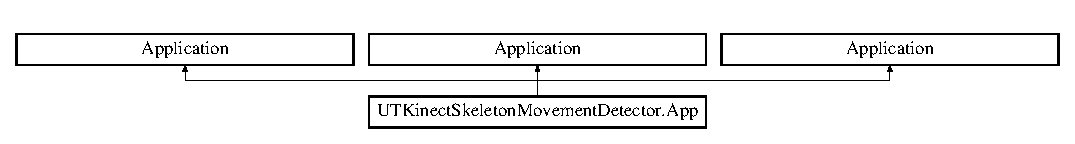
\includegraphics[height=1.487384cm]{classUTKinectSkeletonMovementDetector_1_1App}
\end{center}
\end{figure}
\subsection*{Public Member Functions}
\begin{DoxyCompactItemize}
\item 
void \hyperlink{classUTKinectSkeletonMovementDetector_1_1App_ad4f6df536dd24c00b8fdd75c73eb0988}{Initialize\-Component} ()
\begin{DoxyCompactList}\small\item\em Initialize\-Component \end{DoxyCompactList}\item 
void \hyperlink{classUTKinectSkeletonMovementDetector_1_1App_ad4f6df536dd24c00b8fdd75c73eb0988}{Initialize\-Component} ()
\begin{DoxyCompactList}\small\item\em Initialize\-Component \end{DoxyCompactList}\end{DoxyCompactItemize}
\subsection*{Static Public Member Functions}
\begin{DoxyCompactItemize}
\item 
static void \hyperlink{classUTKinectSkeletonMovementDetector_1_1App_acdb1c09f47bfad48eae6c3926122db28}{Main} ()
\begin{DoxyCompactList}\small\item\em Application Entry Point. \end{DoxyCompactList}\item 
static void \hyperlink{classUTKinectSkeletonMovementDetector_1_1App_acdb1c09f47bfad48eae6c3926122db28}{Main} ()
\begin{DoxyCompactList}\small\item\em Application Entry Point. \end{DoxyCompactList}\end{DoxyCompactItemize}


\subsection{Detailed Description}
Interaction logic for App.\-xaml 

\hyperlink{classUTKinectSkeletonMovementDetector_1_1App}{App} 

\subsection{Member Function Documentation}
\hypertarget{classUTKinectSkeletonMovementDetector_1_1App_ad4f6df536dd24c00b8fdd75c73eb0988}{\index{U\-T\-Kinect\-Skeleton\-Movement\-Detector\-::\-App@{U\-T\-Kinect\-Skeleton\-Movement\-Detector\-::\-App}!Initialize\-Component@{Initialize\-Component}}
\index{Initialize\-Component@{Initialize\-Component}!UTKinectSkeletonMovementDetector::App@{U\-T\-Kinect\-Skeleton\-Movement\-Detector\-::\-App}}
\subsubsection[{Initialize\-Component}]{\setlength{\rightskip}{0pt plus 5cm}void U\-T\-Kinect\-Skeleton\-Movement\-Detector.\-App.\-Initialize\-Component (
\begin{DoxyParamCaption}
{}
\end{DoxyParamCaption}
)}}\label{classUTKinectSkeletonMovementDetector_1_1App_ad4f6df536dd24c00b8fdd75c73eb0988}


Initialize\-Component 

\hypertarget{classUTKinectSkeletonMovementDetector_1_1App_ad4f6df536dd24c00b8fdd75c73eb0988}{\index{U\-T\-Kinect\-Skeleton\-Movement\-Detector\-::\-App@{U\-T\-Kinect\-Skeleton\-Movement\-Detector\-::\-App}!Initialize\-Component@{Initialize\-Component}}
\index{Initialize\-Component@{Initialize\-Component}!UTKinectSkeletonMovementDetector::App@{U\-T\-Kinect\-Skeleton\-Movement\-Detector\-::\-App}}
\subsubsection[{Initialize\-Component}]{\setlength{\rightskip}{0pt plus 5cm}void U\-T\-Kinect\-Skeleton\-Movement\-Detector.\-App.\-Initialize\-Component (
\begin{DoxyParamCaption}
{}
\end{DoxyParamCaption}
)}}\label{classUTKinectSkeletonMovementDetector_1_1App_ad4f6df536dd24c00b8fdd75c73eb0988}


Initialize\-Component 

\hypertarget{classUTKinectSkeletonMovementDetector_1_1App_acdb1c09f47bfad48eae6c3926122db28}{\index{U\-T\-Kinect\-Skeleton\-Movement\-Detector\-::\-App@{U\-T\-Kinect\-Skeleton\-Movement\-Detector\-::\-App}!Main@{Main}}
\index{Main@{Main}!UTKinectSkeletonMovementDetector::App@{U\-T\-Kinect\-Skeleton\-Movement\-Detector\-::\-App}}
\subsubsection[{Main}]{\setlength{\rightskip}{0pt plus 5cm}static void U\-T\-Kinect\-Skeleton\-Movement\-Detector.\-App.\-Main (
\begin{DoxyParamCaption}
{}
\end{DoxyParamCaption}
)\hspace{0.3cm}{\ttfamily [static]}}}\label{classUTKinectSkeletonMovementDetector_1_1App_acdb1c09f47bfad48eae6c3926122db28}


Application Entry Point. 

\hypertarget{classUTKinectSkeletonMovementDetector_1_1App_acdb1c09f47bfad48eae6c3926122db28}{\index{U\-T\-Kinect\-Skeleton\-Movement\-Detector\-::\-App@{U\-T\-Kinect\-Skeleton\-Movement\-Detector\-::\-App}!Main@{Main}}
\index{Main@{Main}!UTKinectSkeletonMovementDetector::App@{U\-T\-Kinect\-Skeleton\-Movement\-Detector\-::\-App}}
\subsubsection[{Main}]{\setlength{\rightskip}{0pt plus 5cm}static void U\-T\-Kinect\-Skeleton\-Movement\-Detector.\-App.\-Main (
\begin{DoxyParamCaption}
{}
\end{DoxyParamCaption}
)\hspace{0.3cm}{\ttfamily [static]}}}\label{classUTKinectSkeletonMovementDetector_1_1App_acdb1c09f47bfad48eae6c3926122db28}


Application Entry Point. 



The documentation for this class was generated from the following files\-:\begin{DoxyCompactItemize}
\item 
\hyperlink{App_8xaml_8cs}{App.\-xaml.\-cs}\item 
obj/x86/\-Release/\hyperlink{Release_2App_8g_8cs}{App.\-g.\-cs}\item 
obj/x86/\-Release/\hyperlink{Release_2App_8g_8i_8cs}{App.\-g.\-i.\-cs}\end{DoxyCompactItemize}

\hypertarget{classWpfApplication4_1_1App}{\section{Wpf\-Application4.\-App Class Reference}
\label{classWpfApplication4_1_1App}\index{Wpf\-Application4.\-App@{Wpf\-Application4.\-App}}
}


\hyperlink{classWpfApplication4_1_1App}{App}  


Inheritance diagram for Wpf\-Application4.\-App\-:\begin{figure}[H]
\begin{center}
\leavevmode
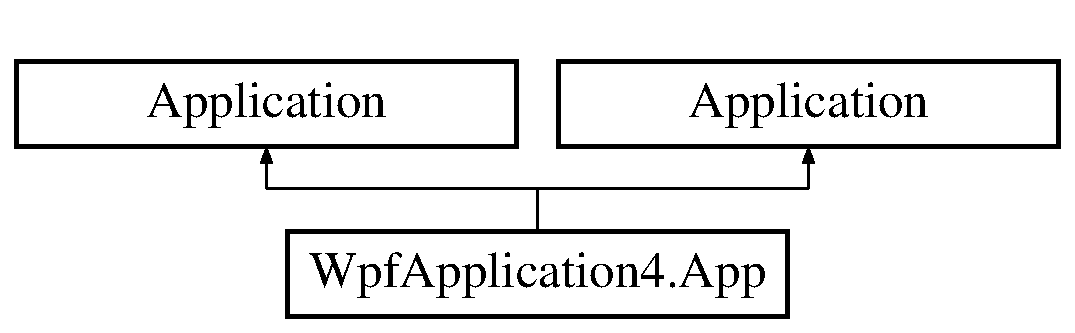
\includegraphics[height=2.000000cm]{classWpfApplication4_1_1App}
\end{center}
\end{figure}
\subsection*{Public Member Functions}
\begin{DoxyCompactItemize}
\item 
void \hyperlink{classWpfApplication4_1_1App_a771c9d33fc561f332b66df12e2df001c}{Initialize\-Component} ()
\begin{DoxyCompactList}\small\item\em Initialize\-Component \end{DoxyCompactList}\item 
void \hyperlink{classWpfApplication4_1_1App_a771c9d33fc561f332b66df12e2df001c}{Initialize\-Component} ()
\begin{DoxyCompactList}\small\item\em Initialize\-Component \end{DoxyCompactList}\end{DoxyCompactItemize}
\subsection*{Static Public Member Functions}
\begin{DoxyCompactItemize}
\item 
static void \hyperlink{classWpfApplication4_1_1App_af9d156f9d05b42856f01e9d71fa7ae9a}{Main} ()
\begin{DoxyCompactList}\small\item\em Application Entry Point. \end{DoxyCompactList}\item 
static void \hyperlink{classWpfApplication4_1_1App_af9d156f9d05b42856f01e9d71fa7ae9a}{Main} ()
\begin{DoxyCompactList}\small\item\em Application Entry Point. \end{DoxyCompactList}\end{DoxyCompactItemize}


\subsection{Detailed Description}
\hyperlink{classWpfApplication4_1_1App}{App} 



\subsection{Member Function Documentation}
\hypertarget{classWpfApplication4_1_1App_a771c9d33fc561f332b66df12e2df001c}{\index{Wpf\-Application4\-::\-App@{Wpf\-Application4\-::\-App}!Initialize\-Component@{Initialize\-Component}}
\index{Initialize\-Component@{Initialize\-Component}!WpfApplication4::App@{Wpf\-Application4\-::\-App}}
\subsubsection[{Initialize\-Component}]{\setlength{\rightskip}{0pt plus 5cm}void Wpf\-Application4.\-App.\-Initialize\-Component (
\begin{DoxyParamCaption}
{}
\end{DoxyParamCaption}
)}}\label{classWpfApplication4_1_1App_a771c9d33fc561f332b66df12e2df001c}


Initialize\-Component 

\hypertarget{classWpfApplication4_1_1App_a771c9d33fc561f332b66df12e2df001c}{\index{Wpf\-Application4\-::\-App@{Wpf\-Application4\-::\-App}!Initialize\-Component@{Initialize\-Component}}
\index{Initialize\-Component@{Initialize\-Component}!WpfApplication4::App@{Wpf\-Application4\-::\-App}}
\subsubsection[{Initialize\-Component}]{\setlength{\rightskip}{0pt plus 5cm}void Wpf\-Application4.\-App.\-Initialize\-Component (
\begin{DoxyParamCaption}
{}
\end{DoxyParamCaption}
)}}\label{classWpfApplication4_1_1App_a771c9d33fc561f332b66df12e2df001c}


Initialize\-Component 

\hypertarget{classWpfApplication4_1_1App_af9d156f9d05b42856f01e9d71fa7ae9a}{\index{Wpf\-Application4\-::\-App@{Wpf\-Application4\-::\-App}!Main@{Main}}
\index{Main@{Main}!WpfApplication4::App@{Wpf\-Application4\-::\-App}}
\subsubsection[{Main}]{\setlength{\rightskip}{0pt plus 5cm}static void Wpf\-Application4.\-App.\-Main (
\begin{DoxyParamCaption}
{}
\end{DoxyParamCaption}
)\hspace{0.3cm}{\ttfamily [static]}}}\label{classWpfApplication4_1_1App_af9d156f9d05b42856f01e9d71fa7ae9a}


Application Entry Point. 

\hypertarget{classWpfApplication4_1_1App_af9d156f9d05b42856f01e9d71fa7ae9a}{\index{Wpf\-Application4\-::\-App@{Wpf\-Application4\-::\-App}!Main@{Main}}
\index{Main@{Main}!WpfApplication4::App@{Wpf\-Application4\-::\-App}}
\subsubsection[{Main}]{\setlength{\rightskip}{0pt plus 5cm}static void Wpf\-Application4.\-App.\-Main (
\begin{DoxyParamCaption}
{}
\end{DoxyParamCaption}
)\hspace{0.3cm}{\ttfamily [static]}}}\label{classWpfApplication4_1_1App_af9d156f9d05b42856f01e9d71fa7ae9a}


Application Entry Point. 



The documentation for this class was generated from the following files\-:\begin{DoxyCompactItemize}
\item 
obj/x86/\-Debug/\hyperlink{Debug_2App_8g_8cs}{App.\-g.\-cs}\item 
obj/x86/\-Debug/\hyperlink{Debug_2App_8g_8i_8cs}{App.\-g.\-i.\-cs}\end{DoxyCompactItemize}

\hypertarget{classUTKinectSkeletonMovementDetector_1_1ColorMovieCreatorWorker}{\section{U\-T\-Kinect\-Skeleton\-Movement\-Detector.\-Color\-Movie\-Creator\-Worker Class Reference}
\label{classUTKinectSkeletonMovementDetector_1_1ColorMovieCreatorWorker}\index{U\-T\-Kinect\-Skeleton\-Movement\-Detector.\-Color\-Movie\-Creator\-Worker@{U\-T\-Kinect\-Skeleton\-Movement\-Detector.\-Color\-Movie\-Creator\-Worker}}
}


color movie creation worker class  


\subsection*{Public Member Functions}
\begin{DoxyCompactItemize}
\item 
delegate void \hyperlink{classUTKinectSkeletonMovementDetector_1_1ColorMovieCreatorWorker_a5bb43499cb3485ff2cc4a139b5f77050}{On\-Worker\-Method\-Complete\-Delegate} (string message)
\item 
\hyperlink{classUTKinectSkeletonMovementDetector_1_1ColorMovieCreatorWorker_a6fa202da9a18d6af550a497cc42378fe}{Color\-Movie\-Creator\-Worker} (List$<$ \hyperlink{classUTKinectSkeletonMovementDetector_1_1MyColorFrame}{My\-Color\-Frame} $>$ cframes, List$<$ \hyperlink{classUTKinectSkeletonMovementDetector_1_1MySkeletonFrame}{My\-Skeleton\-Frame} $>$ sframes, string \hyperlink{classUTKinectSkeletonMovementDetector_1_1ColorMovieCreatorWorker_ace4d34d6ac732c41710967fdcda28b5a}{path})
\begin{DoxyCompactList}\small\item\em cunstructor \end{DoxyCompactList}\item 
void \hyperlink{classUTKinectSkeletonMovementDetector_1_1ColorMovieCreatorWorker_aff3022fbab201ec116d79bdb0a1e6d21}{Worker\-Method} ()
\begin{DoxyCompactList}\small\item\em main method of the worker \end{DoxyCompactList}\end{DoxyCompactItemize}
\subsection*{Events}
\begin{DoxyCompactItemize}
\item 
\hyperlink{classUTKinectSkeletonMovementDetector_1_1ColorMovieCreatorWorker_a5bb43499cb3485ff2cc4a139b5f77050}{On\-Worker\-Method\-Complete\-Delegate} \hyperlink{classUTKinectSkeletonMovementDetector_1_1ColorMovieCreatorWorker_aa3e3f57176cf63366e90893f7095aa83}{On\-Worker\-Complete}
\end{DoxyCompactItemize}
\subsection*{Private Attributes}
\begin{DoxyCompactItemize}
\item 
List$<$ \hyperlink{classUTKinectSkeletonMovementDetector_1_1MyColorFrame}{My\-Color\-Frame} $>$ \hyperlink{classUTKinectSkeletonMovementDetector_1_1ColorMovieCreatorWorker_a6988e4c0c5433ddf9bd8e30923b900d8}{colorframes}
\item 
List$<$ \hyperlink{classUTKinectSkeletonMovementDetector_1_1MySkeletonFrame}{My\-Skeleton\-Frame} $>$ \hyperlink{classUTKinectSkeletonMovementDetector_1_1ColorMovieCreatorWorker_ad638f0391870949347c5bfb74ec1f96d}{skeletonframes}
\item 
string \hyperlink{classUTKinectSkeletonMovementDetector_1_1ColorMovieCreatorWorker_ace4d34d6ac732c41710967fdcda28b5a}{path}
\end{DoxyCompactItemize}


\subsection{Detailed Description}
color movie creation worker class 



\subsection{Constructor \& Destructor Documentation}
\hypertarget{classUTKinectSkeletonMovementDetector_1_1ColorMovieCreatorWorker_a6fa202da9a18d6af550a497cc42378fe}{\index{U\-T\-Kinect\-Skeleton\-Movement\-Detector\-::\-Color\-Movie\-Creator\-Worker@{U\-T\-Kinect\-Skeleton\-Movement\-Detector\-::\-Color\-Movie\-Creator\-Worker}!Color\-Movie\-Creator\-Worker@{Color\-Movie\-Creator\-Worker}}
\index{Color\-Movie\-Creator\-Worker@{Color\-Movie\-Creator\-Worker}!UTKinectSkeletonMovementDetector::ColorMovieCreatorWorker@{U\-T\-Kinect\-Skeleton\-Movement\-Detector\-::\-Color\-Movie\-Creator\-Worker}}
\subsubsection[{Color\-Movie\-Creator\-Worker}]{\setlength{\rightskip}{0pt plus 5cm}U\-T\-Kinect\-Skeleton\-Movement\-Detector.\-Color\-Movie\-Creator\-Worker.\-Color\-Movie\-Creator\-Worker (
\begin{DoxyParamCaption}
\item[{List$<$ {\bf My\-Color\-Frame} $>$}]{cframes, }
\item[{List$<$ {\bf My\-Skeleton\-Frame} $>$}]{sframes, }
\item[{string}]{path}
\end{DoxyParamCaption}
)}}\label{classUTKinectSkeletonMovementDetector_1_1ColorMovieCreatorWorker_a6fa202da9a18d6af550a497cc42378fe}


cunstructor 



\subsection{Member Function Documentation}
\hypertarget{classUTKinectSkeletonMovementDetector_1_1ColorMovieCreatorWorker_a5bb43499cb3485ff2cc4a139b5f77050}{\index{U\-T\-Kinect\-Skeleton\-Movement\-Detector\-::\-Color\-Movie\-Creator\-Worker@{U\-T\-Kinect\-Skeleton\-Movement\-Detector\-::\-Color\-Movie\-Creator\-Worker}!On\-Worker\-Method\-Complete\-Delegate@{On\-Worker\-Method\-Complete\-Delegate}}
\index{On\-Worker\-Method\-Complete\-Delegate@{On\-Worker\-Method\-Complete\-Delegate}!UTKinectSkeletonMovementDetector::ColorMovieCreatorWorker@{U\-T\-Kinect\-Skeleton\-Movement\-Detector\-::\-Color\-Movie\-Creator\-Worker}}
\subsubsection[{On\-Worker\-Method\-Complete\-Delegate}]{\setlength{\rightskip}{0pt plus 5cm}delegate void U\-T\-Kinect\-Skeleton\-Movement\-Detector.\-Color\-Movie\-Creator\-Worker.\-On\-Worker\-Method\-Complete\-Delegate (
\begin{DoxyParamCaption}
\item[{string}]{message}
\end{DoxyParamCaption}
)}}\label{classUTKinectSkeletonMovementDetector_1_1ColorMovieCreatorWorker_a5bb43499cb3485ff2cc4a139b5f77050}
\hypertarget{classUTKinectSkeletonMovementDetector_1_1ColorMovieCreatorWorker_aff3022fbab201ec116d79bdb0a1e6d21}{\index{U\-T\-Kinect\-Skeleton\-Movement\-Detector\-::\-Color\-Movie\-Creator\-Worker@{U\-T\-Kinect\-Skeleton\-Movement\-Detector\-::\-Color\-Movie\-Creator\-Worker}!Worker\-Method@{Worker\-Method}}
\index{Worker\-Method@{Worker\-Method}!UTKinectSkeletonMovementDetector::ColorMovieCreatorWorker@{U\-T\-Kinect\-Skeleton\-Movement\-Detector\-::\-Color\-Movie\-Creator\-Worker}}
\subsubsection[{Worker\-Method}]{\setlength{\rightskip}{0pt plus 5cm}void U\-T\-Kinect\-Skeleton\-Movement\-Detector.\-Color\-Movie\-Creator\-Worker.\-Worker\-Method (
\begin{DoxyParamCaption}
{}
\end{DoxyParamCaption}
)}}\label{classUTKinectSkeletonMovementDetector_1_1ColorMovieCreatorWorker_aff3022fbab201ec116d79bdb0a1e6d21}


main method of the worker 



\subsection{Member Data Documentation}
\hypertarget{classUTKinectSkeletonMovementDetector_1_1ColorMovieCreatorWorker_a6988e4c0c5433ddf9bd8e30923b900d8}{\index{U\-T\-Kinect\-Skeleton\-Movement\-Detector\-::\-Color\-Movie\-Creator\-Worker@{U\-T\-Kinect\-Skeleton\-Movement\-Detector\-::\-Color\-Movie\-Creator\-Worker}!colorframes@{colorframes}}
\index{colorframes@{colorframes}!UTKinectSkeletonMovementDetector::ColorMovieCreatorWorker@{U\-T\-Kinect\-Skeleton\-Movement\-Detector\-::\-Color\-Movie\-Creator\-Worker}}
\subsubsection[{colorframes}]{\setlength{\rightskip}{0pt plus 5cm}List$<${\bf My\-Color\-Frame}$>$ U\-T\-Kinect\-Skeleton\-Movement\-Detector.\-Color\-Movie\-Creator\-Worker.\-colorframes\hspace{0.3cm}{\ttfamily [private]}}}\label{classUTKinectSkeletonMovementDetector_1_1ColorMovieCreatorWorker_a6988e4c0c5433ddf9bd8e30923b900d8}
\hypertarget{classUTKinectSkeletonMovementDetector_1_1ColorMovieCreatorWorker_ace4d34d6ac732c41710967fdcda28b5a}{\index{U\-T\-Kinect\-Skeleton\-Movement\-Detector\-::\-Color\-Movie\-Creator\-Worker@{U\-T\-Kinect\-Skeleton\-Movement\-Detector\-::\-Color\-Movie\-Creator\-Worker}!path@{path}}
\index{path@{path}!UTKinectSkeletonMovementDetector::ColorMovieCreatorWorker@{U\-T\-Kinect\-Skeleton\-Movement\-Detector\-::\-Color\-Movie\-Creator\-Worker}}
\subsubsection[{path}]{\setlength{\rightskip}{0pt plus 5cm}string U\-T\-Kinect\-Skeleton\-Movement\-Detector.\-Color\-Movie\-Creator\-Worker.\-path\hspace{0.3cm}{\ttfamily [private]}}}\label{classUTKinectSkeletonMovementDetector_1_1ColorMovieCreatorWorker_ace4d34d6ac732c41710967fdcda28b5a}
\hypertarget{classUTKinectSkeletonMovementDetector_1_1ColorMovieCreatorWorker_ad638f0391870949347c5bfb74ec1f96d}{\index{U\-T\-Kinect\-Skeleton\-Movement\-Detector\-::\-Color\-Movie\-Creator\-Worker@{U\-T\-Kinect\-Skeleton\-Movement\-Detector\-::\-Color\-Movie\-Creator\-Worker}!skeletonframes@{skeletonframes}}
\index{skeletonframes@{skeletonframes}!UTKinectSkeletonMovementDetector::ColorMovieCreatorWorker@{U\-T\-Kinect\-Skeleton\-Movement\-Detector\-::\-Color\-Movie\-Creator\-Worker}}
\subsubsection[{skeletonframes}]{\setlength{\rightskip}{0pt plus 5cm}List$<${\bf My\-Skeleton\-Frame}$>$ U\-T\-Kinect\-Skeleton\-Movement\-Detector.\-Color\-Movie\-Creator\-Worker.\-skeletonframes\hspace{0.3cm}{\ttfamily [private]}}}\label{classUTKinectSkeletonMovementDetector_1_1ColorMovieCreatorWorker_ad638f0391870949347c5bfb74ec1f96d}


\subsection{Event Documentation}
\hypertarget{classUTKinectSkeletonMovementDetector_1_1ColorMovieCreatorWorker_aa3e3f57176cf63366e90893f7095aa83}{\index{U\-T\-Kinect\-Skeleton\-Movement\-Detector\-::\-Color\-Movie\-Creator\-Worker@{U\-T\-Kinect\-Skeleton\-Movement\-Detector\-::\-Color\-Movie\-Creator\-Worker}!On\-Worker\-Complete@{On\-Worker\-Complete}}
\index{On\-Worker\-Complete@{On\-Worker\-Complete}!UTKinectSkeletonMovementDetector::ColorMovieCreatorWorker@{U\-T\-Kinect\-Skeleton\-Movement\-Detector\-::\-Color\-Movie\-Creator\-Worker}}
\subsubsection[{On\-Worker\-Complete}]{\setlength{\rightskip}{0pt plus 5cm}{\bf On\-Worker\-Method\-Complete\-Delegate} U\-T\-Kinect\-Skeleton\-Movement\-Detector.\-Color\-Movie\-Creator\-Worker.\-On\-Worker\-Complete}}\label{classUTKinectSkeletonMovementDetector_1_1ColorMovieCreatorWorker_aa3e3f57176cf63366e90893f7095aa83}


The documentation for this class was generated from the following file\-:\begin{DoxyCompactItemize}
\item 
\hyperlink{ColorMovieCreatorWorker_8cs}{Color\-Movie\-Creator\-Worker.\-cs}\end{DoxyCompactItemize}

\hypertarget{classUTKinectSkeletonMovementDetector_1_1LogService}{\section{U\-T\-Kinect\-Skeleton\-Movement\-Detector.\-Log\-Service Class Reference}
\label{classUTKinectSkeletonMovementDetector_1_1LogService}\index{U\-T\-Kinect\-Skeleton\-Movement\-Detector.\-Log\-Service@{U\-T\-Kinect\-Skeleton\-Movement\-Detector.\-Log\-Service}}
}
\subsection*{Static Public Member Functions}
\begin{DoxyCompactItemize}
\item 
static void \hyperlink{classUTKinectSkeletonMovementDetector_1_1LogService_aa97bb759ae6d3a504f5ff5936e9a91bc}{record\-\_\-logs} (List$<$ \hyperlink{classUTKinectSkeletonMovementDetector_1_1MySkeletonFrame}{My\-Skeleton\-Frame} $>$ skeletonframes, String path)
\end{DoxyCompactItemize}


\subsection{Member Function Documentation}
\hypertarget{classUTKinectSkeletonMovementDetector_1_1LogService_aa97bb759ae6d3a504f5ff5936e9a91bc}{\index{U\-T\-Kinect\-Skeleton\-Movement\-Detector\-::\-Log\-Service@{U\-T\-Kinect\-Skeleton\-Movement\-Detector\-::\-Log\-Service}!record\-\_\-logs@{record\-\_\-logs}}
\index{record\-\_\-logs@{record\-\_\-logs}!UTKinectSkeletonMovementDetector::LogService@{U\-T\-Kinect\-Skeleton\-Movement\-Detector\-::\-Log\-Service}}
\subsubsection[{record\-\_\-logs}]{\setlength{\rightskip}{0pt plus 5cm}static void U\-T\-Kinect\-Skeleton\-Movement\-Detector.\-Log\-Service.\-record\-\_\-logs (
\begin{DoxyParamCaption}
\item[{List$<$ {\bf My\-Skeleton\-Frame} $>$}]{skeletonframes, }
\item[{String}]{path}
\end{DoxyParamCaption}
)\hspace{0.3cm}{\ttfamily [static]}}}\label{classUTKinectSkeletonMovementDetector_1_1LogService_aa97bb759ae6d3a504f5ff5936e9a91bc}


The documentation for this class was generated from the following file\-:\begin{DoxyCompactItemize}
\item 
\hyperlink{LogService_8cs}{Log\-Service.\-cs}\end{DoxyCompactItemize}

\hypertarget{classUTKinectSkeletonMovementDetector_1_1MainWindow}{\section{U\-T\-Kinect\-Skeleton\-Movement\-Detector.\-Main\-Window Class Reference}
\label{classUTKinectSkeletonMovementDetector_1_1MainWindow}\index{U\-T\-Kinect\-Skeleton\-Movement\-Detector.\-Main\-Window@{U\-T\-Kinect\-Skeleton\-Movement\-Detector.\-Main\-Window}}
}


Interaction logic for Main\-Window.\-xaml  


Inheritance diagram for U\-T\-Kinect\-Skeleton\-Movement\-Detector.\-Main\-Window\-:\begin{figure}[H]
\begin{center}
\leavevmode
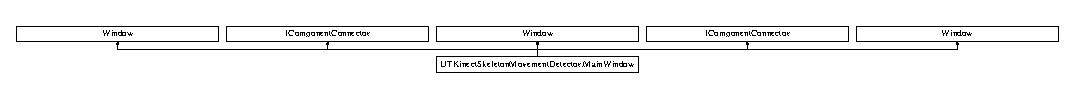
\includegraphics[height=0.746667cm]{classUTKinectSkeletonMovementDetector_1_1MainWindow}
\end{center}
\end{figure}
\subsection*{Public Member Functions}
\begin{DoxyCompactItemize}
\item 
\hyperlink{classUTKinectSkeletonMovementDetector_1_1MainWindow_a5ab15131acc3a1f24f1584232412a5f5}{Main\-Window} ()
\begin{DoxyCompactList}\small\item\em Initializes a new instance of the \hyperlink{classUTKinectSkeletonMovementDetector_1_1MainWindow}{Main\-Window} class. \end{DoxyCompactList}\item 
void \hyperlink{classUTKinectSkeletonMovementDetector_1_1MainWindow_a6b89ad1956b2aba773a1b283632bc047}{Initialize\-Component} ()
\begin{DoxyCompactList}\small\item\em Initialize\-Component \end{DoxyCompactList}\item 
void \hyperlink{classUTKinectSkeletonMovementDetector_1_1MainWindow_a6b89ad1956b2aba773a1b283632bc047}{Initialize\-Component} ()
\begin{DoxyCompactList}\small\item\em Initialize\-Component \end{DoxyCompactList}\end{DoxyCompactItemize}
\subsection*{Package Attributes}
\begin{DoxyCompactItemize}
\item 
System.\-Windows.\-Controls.\-Grid \hyperlink{classUTKinectSkeletonMovementDetector_1_1MainWindow_a46d4c23e930d0705872fd70635bae665}{main\-Grid}
\item 
System.\-Windows.\-Controls.\-Label \hyperlink{classUTKinectSkeletonMovementDetector_1_1MainWindow_a172dcddd5dc71b907f9626554e776978}{overlay\-Background}
\item 
System.\-Windows.\-Controls.\-Image \hyperlink{classUTKinectSkeletonMovementDetector_1_1MainWindow_aae3b6a465781c6d9ed0b82a7e1d43747}{Color\-Image2}
\item 
System.\-Windows.\-Controls.\-Image \hyperlink{classUTKinectSkeletonMovementDetector_1_1MainWindow_ae21b0af522b79668c8ac5b0cf3c75dfe}{Skeleton2}
\item 
System.\-Windows.\-Controls.\-Media\-Element \hyperlink{classUTKinectSkeletonMovementDetector_1_1MainWindow_a1e50e8d30594f7981c6c7c358301cd13}{overlayplayer}
\item 
System.\-Windows.\-Controls.\-Text\-Block \hyperlink{classUTKinectSkeletonMovementDetector_1_1MainWindow_a0b448bc865a6b976d21b69c608c8b151}{Overlay\-Text\-Label}
\item 
System.\-Windows.\-Controls.\-Label \hyperlink{classUTKinectSkeletonMovementDetector_1_1MainWindow_a8b899fad7c2174e584a125de7b741b7d}{color\-Image\-Label}
\item 
System.\-Windows.\-Controls.\-Image \hyperlink{classUTKinectSkeletonMovementDetector_1_1MainWindow_a728c5e61f6b85860e5f4a1c50a17bf50}{Color\-Image}
\item 
System.\-Windows.\-Controls.\-Media\-Element \hyperlink{classUTKinectSkeletonMovementDetector_1_1MainWindow_a58c45dd8fca2bc7a80271a66c290edd1}{rgb\-Player}
\item 
System.\-Windows.\-Controls.\-Text\-Block \hyperlink{classUTKinectSkeletonMovementDetector_1_1MainWindow_a72cb0dc6d60075ec8fb0824fd2cf1cd2}{color\-Text\-Label}
\item 
System.\-Windows.\-Controls.\-Label \hyperlink{classUTKinectSkeletonMovementDetector_1_1MainWindow_af7cf24ac85e9a4e6cd0f6b735fe2674b}{skeleton\-Label}
\item 
System.\-Windows.\-Controls.\-Image \hyperlink{classUTKinectSkeletonMovementDetector_1_1MainWindow_aeaae83e3e199c75e2975b19e7f9e881e}{Skeleton}
\item 
System.\-Windows.\-Controls.\-Media\-Element \hyperlink{classUTKinectSkeletonMovementDetector_1_1MainWindow_aa8a284293965f2d8be2528f6ddce07fe}{skeleton\-Player}
\item 
System.\-Windows.\-Controls.\-Text\-Block \hyperlink{classUTKinectSkeletonMovementDetector_1_1MainWindow_a7a273638d2c547d01be972e5702b1f56}{skeleton\-Text\-Label}
\item 
System.\-Windows.\-Controls.\-Grid \hyperlink{classUTKinectSkeletonMovementDetector_1_1MainWindow_aca06038d8f63f2455d1c3a46cdc3f7c0}{Control\-Grid}
\item 
System.\-Windows.\-Controls.\-Button \hyperlink{classUTKinectSkeletonMovementDetector_1_1MainWindow_a86efef4c2a91bce24ea78034fc88ea53}{play\-\_\-button}
\item 
System.\-Windows.\-Controls.\-Slider \hyperlink{classUTKinectSkeletonMovementDetector_1_1MainWindow_a42e53b8dc19d2580b663b5cd9f2717e2}{player\-\_\-slider}
\item 
System.\-Windows.\-Controls.\-Label \hyperlink{classUTKinectSkeletonMovementDetector_1_1MainWindow_a27cf6fcd9bff2ca2f1e8407af00413e3}{color\-\_\-frame\-\_\-label}
\item 
System.\-Windows.\-Controls.\-Button \hyperlink{classUTKinectSkeletonMovementDetector_1_1MainWindow_a380c8a74f48341dd20d1e2fb4580faff}{live\-\_\-button}
\item 
System.\-Windows.\-Controls.\-Button \hyperlink{classUTKinectSkeletonMovementDetector_1_1MainWindow_af4f2a4c396ff6eb6f80d8a2f5dc69895}{record\-\_\-button}
\end{DoxyCompactItemize}
\subsection*{Private Member Functions}
\begin{DoxyCompactItemize}
\item 
void \hyperlink{classUTKinectSkeletonMovementDetector_1_1MainWindow_a0bb043a0d6a0e7f767c18f277a62ff91}{Window\-Loaded} (object sender, Routed\-Event\-Args e)
\begin{DoxyCompactList}\small\item\em Execute startup tasks \end{DoxyCompactList}\item 
void \hyperlink{classUTKinectSkeletonMovementDetector_1_1MainWindow_a362d7a8479b294a0735e71eef4c9d369}{Window\-Closing} (object sender, System.\-Component\-Model.\-Cancel\-Event\-Args e)
\begin{DoxyCompactList}\small\item\em Execute shutdown tasks \end{DoxyCompactList}\item 
void \hyperlink{classUTKinectSkeletonMovementDetector_1_1MainWindow_a58bec47156e982fc810cb1a8b3aa3369}{Sensor\-Skeleton\-Frame\-Ready} (object sender, Skeleton\-Frame\-Ready\-Event\-Args e)
\begin{DoxyCompactList}\small\item\em runs when new skeleton frame is received \end{DoxyCompactList}\item 
void \hyperlink{classUTKinectSkeletonMovementDetector_1_1MainWindow_a05c77a08fa746cf27d3b2b28bed54a03}{Draw\-Bones\-And\-Joints} (\hyperlink{classUTKinectSkeletonMovementDetector_1_1MainWindow_aeaae83e3e199c75e2975b19e7f9e881e}{Skeleton} skeleton, Drawing\-Context drawing\-Context)
\begin{DoxyCompactList}\small\item\em Draws a skeleton's bones and joints \end{DoxyCompactList}\item 
Point \hyperlink{classUTKinectSkeletonMovementDetector_1_1MainWindow_ace68c6308f144ae17f084bd747fb8073}{Skeleton\-Point\-To\-Screen} (Skeleton\-Point skelpoint)
\begin{DoxyCompactList}\small\item\em Maps a Skeleton\-Point to lie within our render space and converts to Point \end{DoxyCompactList}\item 
void \hyperlink{classUTKinectSkeletonMovementDetector_1_1MainWindow_a8bc4e46bf5d40db49eb2bacb339604b8}{Draw\-Bone} (\hyperlink{classUTKinectSkeletonMovementDetector_1_1MainWindow_aeaae83e3e199c75e2975b19e7f9e881e}{Skeleton} skeleton, Drawing\-Context drawing\-Context, Joint\-Type joint\-Type0, Joint\-Type joint\-Type1)
\begin{DoxyCompactList}\small\item\em Draws a bone line between two joints \end{DoxyCompactList}\item 
void \hyperlink{classUTKinectSkeletonMovementDetector_1_1MainWindow_a6f616ab01ec4ad3f0c0a3b31d1d47fe8}{Sensor\-Color\-Frame\-Ready} (object sender, Color\-Image\-Frame\-Ready\-Event\-Args e)
\begin{DoxyCompactList}\small\item\em runs when new color frame is received \end{DoxyCompactList}\item 
void \hyperlink{classUTKinectSkeletonMovementDetector_1_1MainWindow_a6ec33e1f54a6e9ebf73872f913b259b6}{live\-\_\-button\-\_\-\-Click} (object sender, Routed\-Event\-Args e)
\begin{DoxyCompactList}\small\item\em runs when live button is clicked \end{DoxyCompactList}\item 
bool \hyperlink{classUTKinectSkeletonMovementDetector_1_1MainWindow_aa6851d45043318d1c46f38a46de4ac52}{toggle\-\_\-live} ()
\begin{DoxyCompactList}\small\item\em if sensors are already off this makes them go on and viseversa \end{DoxyCompactList}\item 
bool \hyperlink{classUTKinectSkeletonMovementDetector_1_1MainWindow_a1f752843e3733066b6fadeb7afa9614d}{turn\-\_\-on\-\_\-live\-\_\-observation} ()
\begin{DoxyCompactList}\small\item\em turns on kinect sensors \end{DoxyCompactList}\item 
void \hyperlink{classUTKinectSkeletonMovementDetector_1_1MainWindow_ababdd6965867a2b7eb106d56612b47ef}{turn\-\_\-off\-\_\-live\-\_\-observation} ()
\begin{DoxyCompactList}\small\item\em turns off kinect sensors \end{DoxyCompactList}\item 
void \hyperlink{classUTKinectSkeletonMovementDetector_1_1MainWindow_a62e275c41f9a07b84b91cb5192be5dc2}{start\-\_\-recording} ()
\begin{DoxyCompactList}\small\item\em with the execution of this function every frame received from now on is recorded \end{DoxyCompactList}\item 
void \hyperlink{classUTKinectSkeletonMovementDetector_1_1MainWindow_a0847209581cf66a51945a1871646ed22}{record\-\_\-button\-\_\-\-Click} (object sender, Routed\-Event\-Args e)
\begin{DoxyCompactList}\small\item\em runs when new record/stop button is clicked \end{DoxyCompactList}\item 
void \hyperlink{classUTKinectSkeletonMovementDetector_1_1MainWindow_ac8729c33290d9d0789c9d9f96ce40aa8}{start\-Overlay\-Movie\-Creation} ()
\begin{DoxyCompactList}\small\item\em shows a waiting dialog and start creation of overlay movie in another thread \end{DoxyCompactList}\item 
void \hyperlink{classUTKinectSkeletonMovementDetector_1_1MainWindow_ac3ba79a229a46ae04ff26002d5d246ed}{On\-Overlay\-Worker\-Method\-Complete} (string message)
\begin{DoxyCompactList}\small\item\em runs on overlay movie creation complete, continues with color movie creation process \end{DoxyCompactList}\item 
void \hyperlink{classUTKinectSkeletonMovementDetector_1_1MainWindow_a66411f588ba5705ca061637de3c60891}{start\-Color\-Movie\-Creation} ()
\begin{DoxyCompactList}\small\item\em shows a waiting dialog and start creation of color movie in another thread \end{DoxyCompactList}\item 
void \hyperlink{classUTKinectSkeletonMovementDetector_1_1MainWindow_a854069a07e92baa8a974b7f9f56691ff}{On\-Color\-Worker\-Method\-Complete} (string message)
\begin{DoxyCompactList}\small\item\em runs on color movie creation complete, continues with skeleton movie creation process \end{DoxyCompactList}\item 
void \hyperlink{classUTKinectSkeletonMovementDetector_1_1MainWindow_ada70104856b385a3fd1d03a46987570e}{start\-Skeleton\-Movie\-Creation} ()
\begin{DoxyCompactList}\small\item\em shows a waiting dialog and start creation of skeleton movie in another thread \end{DoxyCompactList}\item 
void \hyperlink{classUTKinectSkeletonMovementDetector_1_1MainWindow_ad60b1ff9b5a4f6ea1c934e291b09bbaa}{On\-Skeleton\-Worker\-Method\-Complete} (string message)
\begin{DoxyCompactList}\small\item\em runs on skeleton creation complete, continues with log creation process \end{DoxyCompactList}\item 
void \hyperlink{classUTKinectSkeletonMovementDetector_1_1MainWindow_a2e5242783864ab44a19fefcad0bbf7f3}{start\-Movement\-Log\-Creation} ()
\begin{DoxyCompactList}\small\item\em shows a waiting dialog and start creation of movement log file in another thread \end{DoxyCompactList}\item 
void \hyperlink{classUTKinectSkeletonMovementDetector_1_1MainWindow_a1874575832de16a05af93078516a60f6}{On\-Log\-Worker\-Method\-Complete} (string message)
\begin{DoxyCompactList}\small\item\em runs on movement log creation complete \end{DoxyCompactList}\item 
void \hyperlink{classUTKinectSkeletonMovementDetector_1_1MainWindow_aa9b03c8c92baa687cb0bc6d8e42839a2}{play\-\_\-button\-\_\-\-Click} (object sender, Routed\-Event\-Args e)
\begin{DoxyCompactList}\small\item\em brings a folder browser dialog and plays all recorded data in there \end{DoxyCompactList}\item 
void \\*
System.\-Windows.\-Markup.\-I\-Component\-Connector. \hyperlink{classUTKinectSkeletonMovementDetector_1_1MainWindow_a3d7ae964fe7e184f9324c6e256b562a0}{Connect} (int connection\-Id, object target)
\item 
void \\*
System.\-Windows.\-Markup.\-I\-Component\-Connector. \hyperlink{classUTKinectSkeletonMovementDetector_1_1MainWindow_a3d7ae964fe7e184f9324c6e256b562a0}{Connect} (int connection\-Id, object target)
\end{DoxyCompactItemize}
\subsection*{Static Private Member Functions}
\begin{DoxyCompactItemize}
\item 
static void \hyperlink{classUTKinectSkeletonMovementDetector_1_1MainWindow_af7e8ffb0ba77dd3a298b0f88f7f33cdb}{Render\-Clipped\-Edges} (\hyperlink{classUTKinectSkeletonMovementDetector_1_1MainWindow_aeaae83e3e199c75e2975b19e7f9e881e}{Skeleton} skeleton, Drawing\-Context drawing\-Context)
\begin{DoxyCompactList}\small\item\em Draws indicators to show which edges are clipping skeleton data \end{DoxyCompactList}\end{DoxyCompactItemize}
\subsection*{Private Attributes}
\begin{DoxyCompactItemize}
\item 
Writeable\-Bitmap \hyperlink{classUTKinectSkeletonMovementDetector_1_1MainWindow_a6518d4a9f673ea5af3a052cf1b31043b}{color\-Bitmap}
\begin{DoxyCompactList}\small\item\em current color frame as bitmap \end{DoxyCompactList}\item 
bool \hyperlink{classUTKinectSkeletonMovementDetector_1_1MainWindow_a08ada1dc46136646bf1929a1f685fd5c}{is\-\_\-recording} = false
\begin{DoxyCompactList}\small\item\em recording status of the moment \end{DoxyCompactList}\item 
List$<$ \hyperlink{classUTKinectSkeletonMovementDetector_1_1MySkeletonFrame}{My\-Skeleton\-Frame} $>$ \hyperlink{classUTKinectSkeletonMovementDetector_1_1MainWindow_a09bd035aa72d079cd6bce48085d9a5fa}{recorded\-\_\-skeleton\-\_\-frames}
\begin{DoxyCompactList}\small\item\em collects all recorded skeleton frames \end{DoxyCompactList}\item 
List$<$ \hyperlink{classUTKinectSkeletonMovementDetector_1_1MyColorFrame}{My\-Color\-Frame} $>$ \hyperlink{classUTKinectSkeletonMovementDetector_1_1MainWindow_a43355bd45cd3d523855a791f01fd5c89}{recorded\-\_\-color\-\_\-frames}
\begin{DoxyCompactList}\small\item\em collects all recorded color frames \end{DoxyCompactList}\item 
String \hyperlink{classUTKinectSkeletonMovementDetector_1_1MainWindow_a5f6b2103e33a42b3f88cf7432c42f44a}{selected\-Path} = \char`\"{}\char`\"{}
\begin{DoxyCompactList}\small\item\em Path selected through path selection dialog \end{DoxyCompactList}\item 
byte\mbox{[}$\,$\mbox{]} \hyperlink{classUTKinectSkeletonMovementDetector_1_1MainWindow_a8c2c29bff1f62d8a03e9936f577e44a8}{color\-Pixels}
\begin{DoxyCompactList}\small\item\em Intermediate storage for the color data received from the camera \end{DoxyCompactList}\item 
\hyperlink{classUTKinectSkeletonMovementDetector_1_1progressDialog}{progress\-Dialog} \hyperlink{classUTKinectSkeletonMovementDetector_1_1MainWindow_ad09c9b8b005cbcc09cb7d1acc722d7c4}{progress\-Window}
\begin{DoxyCompactList}\small\item\em Progress dialog which pops up when post processing recorded data \end{DoxyCompactList}\item 
const float \hyperlink{classUTKinectSkeletonMovementDetector_1_1MainWindow_af3b183ca66b6137dfa971ce2bd41ad61}{Render\-Width} = 640.\-0f
\begin{DoxyCompactList}\small\item\em Width of our output drawing \end{DoxyCompactList}\item 
const float \hyperlink{classUTKinectSkeletonMovementDetector_1_1MainWindow_a83c4f5f87333f29e1e75c98b7a6ba80c}{Render\-Height} = 480.\-0f
\begin{DoxyCompactList}\small\item\em Height of our output drawing \end{DoxyCompactList}\item 
const double \hyperlink{classUTKinectSkeletonMovementDetector_1_1MainWindow_a79ff56663c69c70ea3fa5045d5e37e8b}{Joint\-Thickness} = 3
\begin{DoxyCompactList}\small\item\em Thickness of drawn joint lines \end{DoxyCompactList}\item 
const double \hyperlink{classUTKinectSkeletonMovementDetector_1_1MainWindow_a4f6e1744c877ad860f7ee45ba26b87b8}{Body\-Center\-Thickness} = 10
\begin{DoxyCompactList}\small\item\em Thickness of body center ellipse \end{DoxyCompactList}\item 
const double \hyperlink{classUTKinectSkeletonMovementDetector_1_1MainWindow_a6a0ec4c0958b940fb49cc8ca8a5748c6}{Clip\-Bounds\-Thickness} = 10
\begin{DoxyCompactList}\small\item\em Thickness of clip edge rectangles \end{DoxyCompactList}\item 
bool \hyperlink{classUTKinectSkeletonMovementDetector_1_1MainWindow_a8b1de4d1921f6154890c30a8729f4f47}{is\-\_\-observing\-\_\-live} = false
\begin{DoxyCompactList}\small\item\em status of kinect sensors activity \end{DoxyCompactList}\item 
readonly Brush \hyperlink{classUTKinectSkeletonMovementDetector_1_1MainWindow_a8bfd26f98eba97fd468e4010f8022cb3}{center\-Point\-Brush} = Brushes.\-Blue
\begin{DoxyCompactList}\small\item\em Brush used to draw skeleton center point \end{DoxyCompactList}\item 
readonly Brush \hyperlink{classUTKinectSkeletonMovementDetector_1_1MainWindow_a32df891deb0a6cbcb5ce39a10b360640}{tracked\-Joint\-Brush} = new Solid\-Color\-Brush(Color.\-From\-Argb(255, 68, 192, 68))
\begin{DoxyCompactList}\small\item\em Brush used for drawing joints that are currently tracked \end{DoxyCompactList}\item 
readonly Brush \hyperlink{classUTKinectSkeletonMovementDetector_1_1MainWindow_a31afb96aa9574c7c64153506a5a1cc3e}{inferred\-Joint\-Brush} = Brushes.\-Yellow
\begin{DoxyCompactList}\small\item\em Brush used for drawing joints that are currently inferred \end{DoxyCompactList}\item 
readonly Pen \hyperlink{classUTKinectSkeletonMovementDetector_1_1MainWindow_a063c1ae116063d9f00ecec5c56157126}{tracked\-Bone\-Pen} = new Pen(Brushes.\-Green, 6)
\begin{DoxyCompactList}\small\item\em Pen used for drawing bones that are currently tracked \end{DoxyCompactList}\item 
readonly Pen \hyperlink{classUTKinectSkeletonMovementDetector_1_1MainWindow_a93d63abebf74565cfd10da87ced63146}{inferred\-Bone\-Pen} = new Pen(Brushes.\-Gray, 1)
\begin{DoxyCompactList}\small\item\em Pen used for drawing bones that are currently inferred \end{DoxyCompactList}\item 
Kinect\-Sensor \hyperlink{classUTKinectSkeletonMovementDetector_1_1MainWindow_a12079fceab599014f7f11e5384617cee}{sensor}
\begin{DoxyCompactList}\small\item\em Active Kinect sensor \end{DoxyCompactList}\item 
Drawing\-Group \hyperlink{classUTKinectSkeletonMovementDetector_1_1MainWindow_a6d47dabfa57758770ec1b4772c95535a}{drawing\-Group}
\begin{DoxyCompactList}\small\item\em Drawing group for skeleton rendering output \end{DoxyCompactList}\item 
Drawing\-Group \hyperlink{classUTKinectSkeletonMovementDetector_1_1MainWindow_a6e11f78d0a9135efb206ecfcdbf0a17d}{overlaydrawing\-Group}
\begin{DoxyCompactList}\small\item\em Drawing group for overlay frames rendering output \end{DoxyCompactList}\item 
Drawing\-Image \hyperlink{classUTKinectSkeletonMovementDetector_1_1MainWindow_ad52ff16c5b6e893435ec7395a6c2d629}{image\-Source}
\begin{DoxyCompactList}\small\item\em Drawing image that we will display \end{DoxyCompactList}\item 
Drawing\-Image \hyperlink{classUTKinectSkeletonMovementDetector_1_1MainWindow_acea605090684467d3ae6c5df480c63f5}{overlayimage\-Source}
\begin{DoxyCompactList}\small\item\em Drawing overlay image that we will display \end{DoxyCompactList}\item 
bool \hyperlink{classUTKinectSkeletonMovementDetector_1_1MainWindow_ad0b36121811c03d7419565086eef94b4}{\-\_\-content\-Loaded}
\end{DoxyCompactItemize}


\subsection{Detailed Description}
Interaction logic for Main\-Window.\-xaml 

\hyperlink{classUTKinectSkeletonMovementDetector_1_1MainWindow}{Main\-Window} 

\subsection{Constructor \& Destructor Documentation}
\hypertarget{classUTKinectSkeletonMovementDetector_1_1MainWindow_a5ab15131acc3a1f24f1584232412a5f5}{\index{U\-T\-Kinect\-Skeleton\-Movement\-Detector\-::\-Main\-Window@{U\-T\-Kinect\-Skeleton\-Movement\-Detector\-::\-Main\-Window}!Main\-Window@{Main\-Window}}
\index{Main\-Window@{Main\-Window}!UTKinectSkeletonMovementDetector::MainWindow@{U\-T\-Kinect\-Skeleton\-Movement\-Detector\-::\-Main\-Window}}
\subsubsection[{Main\-Window}]{\setlength{\rightskip}{0pt plus 5cm}U\-T\-Kinect\-Skeleton\-Movement\-Detector.\-Main\-Window.\-Main\-Window (
\begin{DoxyParamCaption}
{}
\end{DoxyParamCaption}
)}}\label{classUTKinectSkeletonMovementDetector_1_1MainWindow_a5ab15131acc3a1f24f1584232412a5f5}


Initializes a new instance of the \hyperlink{classUTKinectSkeletonMovementDetector_1_1MainWindow}{Main\-Window} class. 



\subsection{Member Function Documentation}
\hypertarget{classUTKinectSkeletonMovementDetector_1_1MainWindow_a3d7ae964fe7e184f9324c6e256b562a0}{\index{U\-T\-Kinect\-Skeleton\-Movement\-Detector\-::\-Main\-Window@{U\-T\-Kinect\-Skeleton\-Movement\-Detector\-::\-Main\-Window}!Connect@{Connect}}
\index{Connect@{Connect}!UTKinectSkeletonMovementDetector::MainWindow@{U\-T\-Kinect\-Skeleton\-Movement\-Detector\-::\-Main\-Window}}
\subsubsection[{Connect}]{\setlength{\rightskip}{0pt plus 5cm}void System.\-Windows.\-Markup.\-I\-Component\-Connector. U\-T\-Kinect\-Skeleton\-Movement\-Detector.\-Main\-Window.\-Connect (
\begin{DoxyParamCaption}
\item[{int}]{connection\-Id, }
\item[{object}]{target}
\end{DoxyParamCaption}
)\hspace{0.3cm}{\ttfamily [private]}}}\label{classUTKinectSkeletonMovementDetector_1_1MainWindow_a3d7ae964fe7e184f9324c6e256b562a0}
\hypertarget{classUTKinectSkeletonMovementDetector_1_1MainWindow_a3d7ae964fe7e184f9324c6e256b562a0}{\index{U\-T\-Kinect\-Skeleton\-Movement\-Detector\-::\-Main\-Window@{U\-T\-Kinect\-Skeleton\-Movement\-Detector\-::\-Main\-Window}!Connect@{Connect}}
\index{Connect@{Connect}!UTKinectSkeletonMovementDetector::MainWindow@{U\-T\-Kinect\-Skeleton\-Movement\-Detector\-::\-Main\-Window}}
\subsubsection[{Connect}]{\setlength{\rightskip}{0pt plus 5cm}void System.\-Windows.\-Markup.\-I\-Component\-Connector. U\-T\-Kinect\-Skeleton\-Movement\-Detector.\-Main\-Window.\-Connect (
\begin{DoxyParamCaption}
\item[{int}]{connection\-Id, }
\item[{object}]{target}
\end{DoxyParamCaption}
)\hspace{0.3cm}{\ttfamily [private]}}}\label{classUTKinectSkeletonMovementDetector_1_1MainWindow_a3d7ae964fe7e184f9324c6e256b562a0}
\hypertarget{classUTKinectSkeletonMovementDetector_1_1MainWindow_a8bc4e46bf5d40db49eb2bacb339604b8}{\index{U\-T\-Kinect\-Skeleton\-Movement\-Detector\-::\-Main\-Window@{U\-T\-Kinect\-Skeleton\-Movement\-Detector\-::\-Main\-Window}!Draw\-Bone@{Draw\-Bone}}
\index{Draw\-Bone@{Draw\-Bone}!UTKinectSkeletonMovementDetector::MainWindow@{U\-T\-Kinect\-Skeleton\-Movement\-Detector\-::\-Main\-Window}}
\subsubsection[{Draw\-Bone}]{\setlength{\rightskip}{0pt plus 5cm}void U\-T\-Kinect\-Skeleton\-Movement\-Detector.\-Main\-Window.\-Draw\-Bone (
\begin{DoxyParamCaption}
\item[{{\bf Skeleton}}]{skeleton, }
\item[{Drawing\-Context}]{drawing\-Context, }
\item[{Joint\-Type}]{joint\-Type0, }
\item[{Joint\-Type}]{joint\-Type1}
\end{DoxyParamCaption}
)\hspace{0.3cm}{\ttfamily [private]}}}\label{classUTKinectSkeletonMovementDetector_1_1MainWindow_a8bc4e46bf5d40db49eb2bacb339604b8}


Draws a bone line between two joints 


\begin{DoxyParams}{Parameters}
{\em skeleton} & skeleton to draw bones from\\
\hline
{\em drawing\-Context} & drawing context to draw to\\
\hline
{\em joint\-Type0} & joint to start drawing from\\
\hline
{\em joint\-Type1} & joint to end drawing at\\
\hline
\end{DoxyParams}
\hypertarget{classUTKinectSkeletonMovementDetector_1_1MainWindow_a05c77a08fa746cf27d3b2b28bed54a03}{\index{U\-T\-Kinect\-Skeleton\-Movement\-Detector\-::\-Main\-Window@{U\-T\-Kinect\-Skeleton\-Movement\-Detector\-::\-Main\-Window}!Draw\-Bones\-And\-Joints@{Draw\-Bones\-And\-Joints}}
\index{Draw\-Bones\-And\-Joints@{Draw\-Bones\-And\-Joints}!UTKinectSkeletonMovementDetector::MainWindow@{U\-T\-Kinect\-Skeleton\-Movement\-Detector\-::\-Main\-Window}}
\subsubsection[{Draw\-Bones\-And\-Joints}]{\setlength{\rightskip}{0pt plus 5cm}void U\-T\-Kinect\-Skeleton\-Movement\-Detector.\-Main\-Window.\-Draw\-Bones\-And\-Joints (
\begin{DoxyParamCaption}
\item[{{\bf Skeleton}}]{skeleton, }
\item[{Drawing\-Context}]{drawing\-Context}
\end{DoxyParamCaption}
)\hspace{0.3cm}{\ttfamily [private]}}}\label{classUTKinectSkeletonMovementDetector_1_1MainWindow_a05c77a08fa746cf27d3b2b28bed54a03}


Draws a skeleton's bones and joints 


\begin{DoxyParams}{Parameters}
{\em skeleton} & skeleton to draw\\
\hline
{\em drawing\-Context} & drawing context to draw to\\
\hline
\end{DoxyParams}
\hypertarget{classUTKinectSkeletonMovementDetector_1_1MainWindow_a6b89ad1956b2aba773a1b283632bc047}{\index{U\-T\-Kinect\-Skeleton\-Movement\-Detector\-::\-Main\-Window@{U\-T\-Kinect\-Skeleton\-Movement\-Detector\-::\-Main\-Window}!Initialize\-Component@{Initialize\-Component}}
\index{Initialize\-Component@{Initialize\-Component}!UTKinectSkeletonMovementDetector::MainWindow@{U\-T\-Kinect\-Skeleton\-Movement\-Detector\-::\-Main\-Window}}
\subsubsection[{Initialize\-Component}]{\setlength{\rightskip}{0pt plus 5cm}void U\-T\-Kinect\-Skeleton\-Movement\-Detector.\-Main\-Window.\-Initialize\-Component (
\begin{DoxyParamCaption}
{}
\end{DoxyParamCaption}
)}}\label{classUTKinectSkeletonMovementDetector_1_1MainWindow_a6b89ad1956b2aba773a1b283632bc047}


Initialize\-Component 

\hypertarget{classUTKinectSkeletonMovementDetector_1_1MainWindow_a6b89ad1956b2aba773a1b283632bc047}{\index{U\-T\-Kinect\-Skeleton\-Movement\-Detector\-::\-Main\-Window@{U\-T\-Kinect\-Skeleton\-Movement\-Detector\-::\-Main\-Window}!Initialize\-Component@{Initialize\-Component}}
\index{Initialize\-Component@{Initialize\-Component}!UTKinectSkeletonMovementDetector::MainWindow@{U\-T\-Kinect\-Skeleton\-Movement\-Detector\-::\-Main\-Window}}
\subsubsection[{Initialize\-Component}]{\setlength{\rightskip}{0pt plus 5cm}void U\-T\-Kinect\-Skeleton\-Movement\-Detector.\-Main\-Window.\-Initialize\-Component (
\begin{DoxyParamCaption}
{}
\end{DoxyParamCaption}
)}}\label{classUTKinectSkeletonMovementDetector_1_1MainWindow_a6b89ad1956b2aba773a1b283632bc047}


Initialize\-Component 

\hypertarget{classUTKinectSkeletonMovementDetector_1_1MainWindow_a6ec33e1f54a6e9ebf73872f913b259b6}{\index{U\-T\-Kinect\-Skeleton\-Movement\-Detector\-::\-Main\-Window@{U\-T\-Kinect\-Skeleton\-Movement\-Detector\-::\-Main\-Window}!live\-\_\-button\-\_\-\-Click@{live\-\_\-button\-\_\-\-Click}}
\index{live\-\_\-button\-\_\-\-Click@{live\-\_\-button\-\_\-\-Click}!UTKinectSkeletonMovementDetector::MainWindow@{U\-T\-Kinect\-Skeleton\-Movement\-Detector\-::\-Main\-Window}}
\subsubsection[{live\-\_\-button\-\_\-\-Click}]{\setlength{\rightskip}{0pt plus 5cm}void U\-T\-Kinect\-Skeleton\-Movement\-Detector.\-Main\-Window.\-live\-\_\-button\-\_\-\-Click (
\begin{DoxyParamCaption}
\item[{object}]{sender, }
\item[{Routed\-Event\-Args}]{e}
\end{DoxyParamCaption}
)\hspace{0.3cm}{\ttfamily [private]}}}\label{classUTKinectSkeletonMovementDetector_1_1MainWindow_a6ec33e1f54a6e9ebf73872f913b259b6}


runs when live button is clicked 


\begin{DoxyParams}{Parameters}
{\em sender} & object sending the event\\
\hline
{\em e} & event arguments\\
\hline
\end{DoxyParams}
\hypertarget{classUTKinectSkeletonMovementDetector_1_1MainWindow_a854069a07e92baa8a974b7f9f56691ff}{\index{U\-T\-Kinect\-Skeleton\-Movement\-Detector\-::\-Main\-Window@{U\-T\-Kinect\-Skeleton\-Movement\-Detector\-::\-Main\-Window}!On\-Color\-Worker\-Method\-Complete@{On\-Color\-Worker\-Method\-Complete}}
\index{On\-Color\-Worker\-Method\-Complete@{On\-Color\-Worker\-Method\-Complete}!UTKinectSkeletonMovementDetector::MainWindow@{U\-T\-Kinect\-Skeleton\-Movement\-Detector\-::\-Main\-Window}}
\subsubsection[{On\-Color\-Worker\-Method\-Complete}]{\setlength{\rightskip}{0pt plus 5cm}void U\-T\-Kinect\-Skeleton\-Movement\-Detector.\-Main\-Window.\-On\-Color\-Worker\-Method\-Complete (
\begin{DoxyParamCaption}
\item[{string}]{message}
\end{DoxyParamCaption}
)\hspace{0.3cm}{\ttfamily [private]}}}\label{classUTKinectSkeletonMovementDetector_1_1MainWindow_a854069a07e92baa8a974b7f9f56691ff}


runs on color movie creation complete, continues with skeleton movie creation process 

\hypertarget{classUTKinectSkeletonMovementDetector_1_1MainWindow_a1874575832de16a05af93078516a60f6}{\index{U\-T\-Kinect\-Skeleton\-Movement\-Detector\-::\-Main\-Window@{U\-T\-Kinect\-Skeleton\-Movement\-Detector\-::\-Main\-Window}!On\-Log\-Worker\-Method\-Complete@{On\-Log\-Worker\-Method\-Complete}}
\index{On\-Log\-Worker\-Method\-Complete@{On\-Log\-Worker\-Method\-Complete}!UTKinectSkeletonMovementDetector::MainWindow@{U\-T\-Kinect\-Skeleton\-Movement\-Detector\-::\-Main\-Window}}
\subsubsection[{On\-Log\-Worker\-Method\-Complete}]{\setlength{\rightskip}{0pt plus 5cm}void U\-T\-Kinect\-Skeleton\-Movement\-Detector.\-Main\-Window.\-On\-Log\-Worker\-Method\-Complete (
\begin{DoxyParamCaption}
\item[{string}]{message}
\end{DoxyParamCaption}
)\hspace{0.3cm}{\ttfamily [private]}}}\label{classUTKinectSkeletonMovementDetector_1_1MainWindow_a1874575832de16a05af93078516a60f6}


runs on movement log creation complete 

\hypertarget{classUTKinectSkeletonMovementDetector_1_1MainWindow_ac3ba79a229a46ae04ff26002d5d246ed}{\index{U\-T\-Kinect\-Skeleton\-Movement\-Detector\-::\-Main\-Window@{U\-T\-Kinect\-Skeleton\-Movement\-Detector\-::\-Main\-Window}!On\-Overlay\-Worker\-Method\-Complete@{On\-Overlay\-Worker\-Method\-Complete}}
\index{On\-Overlay\-Worker\-Method\-Complete@{On\-Overlay\-Worker\-Method\-Complete}!UTKinectSkeletonMovementDetector::MainWindow@{U\-T\-Kinect\-Skeleton\-Movement\-Detector\-::\-Main\-Window}}
\subsubsection[{On\-Overlay\-Worker\-Method\-Complete}]{\setlength{\rightskip}{0pt plus 5cm}void U\-T\-Kinect\-Skeleton\-Movement\-Detector.\-Main\-Window.\-On\-Overlay\-Worker\-Method\-Complete (
\begin{DoxyParamCaption}
\item[{string}]{message}
\end{DoxyParamCaption}
)\hspace{0.3cm}{\ttfamily [private]}}}\label{classUTKinectSkeletonMovementDetector_1_1MainWindow_ac3ba79a229a46ae04ff26002d5d246ed}


runs on overlay movie creation complete, continues with color movie creation process 

\hypertarget{classUTKinectSkeletonMovementDetector_1_1MainWindow_ad60b1ff9b5a4f6ea1c934e291b09bbaa}{\index{U\-T\-Kinect\-Skeleton\-Movement\-Detector\-::\-Main\-Window@{U\-T\-Kinect\-Skeleton\-Movement\-Detector\-::\-Main\-Window}!On\-Skeleton\-Worker\-Method\-Complete@{On\-Skeleton\-Worker\-Method\-Complete}}
\index{On\-Skeleton\-Worker\-Method\-Complete@{On\-Skeleton\-Worker\-Method\-Complete}!UTKinectSkeletonMovementDetector::MainWindow@{U\-T\-Kinect\-Skeleton\-Movement\-Detector\-::\-Main\-Window}}
\subsubsection[{On\-Skeleton\-Worker\-Method\-Complete}]{\setlength{\rightskip}{0pt plus 5cm}void U\-T\-Kinect\-Skeleton\-Movement\-Detector.\-Main\-Window.\-On\-Skeleton\-Worker\-Method\-Complete (
\begin{DoxyParamCaption}
\item[{string}]{message}
\end{DoxyParamCaption}
)\hspace{0.3cm}{\ttfamily [private]}}}\label{classUTKinectSkeletonMovementDetector_1_1MainWindow_ad60b1ff9b5a4f6ea1c934e291b09bbaa}


runs on skeleton creation complete, continues with log creation process 

\hypertarget{classUTKinectSkeletonMovementDetector_1_1MainWindow_aa9b03c8c92baa687cb0bc6d8e42839a2}{\index{U\-T\-Kinect\-Skeleton\-Movement\-Detector\-::\-Main\-Window@{U\-T\-Kinect\-Skeleton\-Movement\-Detector\-::\-Main\-Window}!play\-\_\-button\-\_\-\-Click@{play\-\_\-button\-\_\-\-Click}}
\index{play\-\_\-button\-\_\-\-Click@{play\-\_\-button\-\_\-\-Click}!UTKinectSkeletonMovementDetector::MainWindow@{U\-T\-Kinect\-Skeleton\-Movement\-Detector\-::\-Main\-Window}}
\subsubsection[{play\-\_\-button\-\_\-\-Click}]{\setlength{\rightskip}{0pt plus 5cm}void U\-T\-Kinect\-Skeleton\-Movement\-Detector.\-Main\-Window.\-play\-\_\-button\-\_\-\-Click (
\begin{DoxyParamCaption}
\item[{object}]{sender, }
\item[{Routed\-Event\-Args}]{e}
\end{DoxyParamCaption}
)\hspace{0.3cm}{\ttfamily [private]}}}\label{classUTKinectSkeletonMovementDetector_1_1MainWindow_aa9b03c8c92baa687cb0bc6d8e42839a2}


brings a folder browser dialog and plays all recorded data in there 

\hypertarget{classUTKinectSkeletonMovementDetector_1_1MainWindow_a0847209581cf66a51945a1871646ed22}{\index{U\-T\-Kinect\-Skeleton\-Movement\-Detector\-::\-Main\-Window@{U\-T\-Kinect\-Skeleton\-Movement\-Detector\-::\-Main\-Window}!record\-\_\-button\-\_\-\-Click@{record\-\_\-button\-\_\-\-Click}}
\index{record\-\_\-button\-\_\-\-Click@{record\-\_\-button\-\_\-\-Click}!UTKinectSkeletonMovementDetector::MainWindow@{U\-T\-Kinect\-Skeleton\-Movement\-Detector\-::\-Main\-Window}}
\subsubsection[{record\-\_\-button\-\_\-\-Click}]{\setlength{\rightskip}{0pt plus 5cm}void U\-T\-Kinect\-Skeleton\-Movement\-Detector.\-Main\-Window.\-record\-\_\-button\-\_\-\-Click (
\begin{DoxyParamCaption}
\item[{object}]{sender, }
\item[{Routed\-Event\-Args}]{e}
\end{DoxyParamCaption}
)\hspace{0.3cm}{\ttfamily [private]}}}\label{classUTKinectSkeletonMovementDetector_1_1MainWindow_a0847209581cf66a51945a1871646ed22}


runs when new record/stop button is clicked 


\begin{DoxyParams}{Parameters}
{\em sender} & object sending the event\\
\hline
{\em e} & event arguments\\
\hline
\end{DoxyParams}
\hypertarget{classUTKinectSkeletonMovementDetector_1_1MainWindow_af7e8ffb0ba77dd3a298b0f88f7f33cdb}{\index{U\-T\-Kinect\-Skeleton\-Movement\-Detector\-::\-Main\-Window@{U\-T\-Kinect\-Skeleton\-Movement\-Detector\-::\-Main\-Window}!Render\-Clipped\-Edges@{Render\-Clipped\-Edges}}
\index{Render\-Clipped\-Edges@{Render\-Clipped\-Edges}!UTKinectSkeletonMovementDetector::MainWindow@{U\-T\-Kinect\-Skeleton\-Movement\-Detector\-::\-Main\-Window}}
\subsubsection[{Render\-Clipped\-Edges}]{\setlength{\rightskip}{0pt plus 5cm}static void U\-T\-Kinect\-Skeleton\-Movement\-Detector.\-Main\-Window.\-Render\-Clipped\-Edges (
\begin{DoxyParamCaption}
\item[{{\bf Skeleton}}]{skeleton, }
\item[{Drawing\-Context}]{drawing\-Context}
\end{DoxyParamCaption}
)\hspace{0.3cm}{\ttfamily [static]}, {\ttfamily [private]}}}\label{classUTKinectSkeletonMovementDetector_1_1MainWindow_af7e8ffb0ba77dd3a298b0f88f7f33cdb}


Draws indicators to show which edges are clipping skeleton data 


\begin{DoxyParams}{Parameters}
{\em skeleton} & skeleton to draw clipping information for\\
\hline
{\em drawing\-Context} & drawing context to draw to\\
\hline
\end{DoxyParams}
\hypertarget{classUTKinectSkeletonMovementDetector_1_1MainWindow_a6f616ab01ec4ad3f0c0a3b31d1d47fe8}{\index{U\-T\-Kinect\-Skeleton\-Movement\-Detector\-::\-Main\-Window@{U\-T\-Kinect\-Skeleton\-Movement\-Detector\-::\-Main\-Window}!Sensor\-Color\-Frame\-Ready@{Sensor\-Color\-Frame\-Ready}}
\index{Sensor\-Color\-Frame\-Ready@{Sensor\-Color\-Frame\-Ready}!UTKinectSkeletonMovementDetector::MainWindow@{U\-T\-Kinect\-Skeleton\-Movement\-Detector\-::\-Main\-Window}}
\subsubsection[{Sensor\-Color\-Frame\-Ready}]{\setlength{\rightskip}{0pt plus 5cm}void U\-T\-Kinect\-Skeleton\-Movement\-Detector.\-Main\-Window.\-Sensor\-Color\-Frame\-Ready (
\begin{DoxyParamCaption}
\item[{object}]{sender, }
\item[{Color\-Image\-Frame\-Ready\-Event\-Args}]{e}
\end{DoxyParamCaption}
)\hspace{0.3cm}{\ttfamily [private]}}}\label{classUTKinectSkeletonMovementDetector_1_1MainWindow_a6f616ab01ec4ad3f0c0a3b31d1d47fe8}


runs when new color frame is received 


\begin{DoxyParams}{Parameters}
{\em sender} & object sending the event\\
\hline
{\em e} & event arguments\\
\hline
\end{DoxyParams}
\hypertarget{classUTKinectSkeletonMovementDetector_1_1MainWindow_a58bec47156e982fc810cb1a8b3aa3369}{\index{U\-T\-Kinect\-Skeleton\-Movement\-Detector\-::\-Main\-Window@{U\-T\-Kinect\-Skeleton\-Movement\-Detector\-::\-Main\-Window}!Sensor\-Skeleton\-Frame\-Ready@{Sensor\-Skeleton\-Frame\-Ready}}
\index{Sensor\-Skeleton\-Frame\-Ready@{Sensor\-Skeleton\-Frame\-Ready}!UTKinectSkeletonMovementDetector::MainWindow@{U\-T\-Kinect\-Skeleton\-Movement\-Detector\-::\-Main\-Window}}
\subsubsection[{Sensor\-Skeleton\-Frame\-Ready}]{\setlength{\rightskip}{0pt plus 5cm}void U\-T\-Kinect\-Skeleton\-Movement\-Detector.\-Main\-Window.\-Sensor\-Skeleton\-Frame\-Ready (
\begin{DoxyParamCaption}
\item[{object}]{sender, }
\item[{Skeleton\-Frame\-Ready\-Event\-Args}]{e}
\end{DoxyParamCaption}
)\hspace{0.3cm}{\ttfamily [private]}}}\label{classUTKinectSkeletonMovementDetector_1_1MainWindow_a58bec47156e982fc810cb1a8b3aa3369}


runs when new skeleton frame is received 


\begin{DoxyParams}{Parameters}
{\em sender} & object sending the event\\
\hline
{\em e} & event arguments\\
\hline
\end{DoxyParams}
\hypertarget{classUTKinectSkeletonMovementDetector_1_1MainWindow_ace68c6308f144ae17f084bd747fb8073}{\index{U\-T\-Kinect\-Skeleton\-Movement\-Detector\-::\-Main\-Window@{U\-T\-Kinect\-Skeleton\-Movement\-Detector\-::\-Main\-Window}!Skeleton\-Point\-To\-Screen@{Skeleton\-Point\-To\-Screen}}
\index{Skeleton\-Point\-To\-Screen@{Skeleton\-Point\-To\-Screen}!UTKinectSkeletonMovementDetector::MainWindow@{U\-T\-Kinect\-Skeleton\-Movement\-Detector\-::\-Main\-Window}}
\subsubsection[{Skeleton\-Point\-To\-Screen}]{\setlength{\rightskip}{0pt plus 5cm}Point U\-T\-Kinect\-Skeleton\-Movement\-Detector.\-Main\-Window.\-Skeleton\-Point\-To\-Screen (
\begin{DoxyParamCaption}
\item[{Skeleton\-Point}]{skelpoint}
\end{DoxyParamCaption}
)\hspace{0.3cm}{\ttfamily [private]}}}\label{classUTKinectSkeletonMovementDetector_1_1MainWindow_ace68c6308f144ae17f084bd747fb8073}


Maps a Skeleton\-Point to lie within our render space and converts to Point 


\begin{DoxyParams}{Parameters}
{\em skelpoint} & point to map\\
\hline
\end{DoxyParams}
\begin{DoxyReturn}{Returns}
mapped point
\end{DoxyReturn}
\hypertarget{classUTKinectSkeletonMovementDetector_1_1MainWindow_a62e275c41f9a07b84b91cb5192be5dc2}{\index{U\-T\-Kinect\-Skeleton\-Movement\-Detector\-::\-Main\-Window@{U\-T\-Kinect\-Skeleton\-Movement\-Detector\-::\-Main\-Window}!start\-\_\-recording@{start\-\_\-recording}}
\index{start\-\_\-recording@{start\-\_\-recording}!UTKinectSkeletonMovementDetector::MainWindow@{U\-T\-Kinect\-Skeleton\-Movement\-Detector\-::\-Main\-Window}}
\subsubsection[{start\-\_\-recording}]{\setlength{\rightskip}{0pt plus 5cm}void U\-T\-Kinect\-Skeleton\-Movement\-Detector.\-Main\-Window.\-start\-\_\-recording (
\begin{DoxyParamCaption}
{}
\end{DoxyParamCaption}
)\hspace{0.3cm}{\ttfamily [private]}}}\label{classUTKinectSkeletonMovementDetector_1_1MainWindow_a62e275c41f9a07b84b91cb5192be5dc2}


with the execution of this function every frame received from now on is recorded 

\hypertarget{classUTKinectSkeletonMovementDetector_1_1MainWindow_a66411f588ba5705ca061637de3c60891}{\index{U\-T\-Kinect\-Skeleton\-Movement\-Detector\-::\-Main\-Window@{U\-T\-Kinect\-Skeleton\-Movement\-Detector\-::\-Main\-Window}!start\-Color\-Movie\-Creation@{start\-Color\-Movie\-Creation}}
\index{start\-Color\-Movie\-Creation@{start\-Color\-Movie\-Creation}!UTKinectSkeletonMovementDetector::MainWindow@{U\-T\-Kinect\-Skeleton\-Movement\-Detector\-::\-Main\-Window}}
\subsubsection[{start\-Color\-Movie\-Creation}]{\setlength{\rightskip}{0pt plus 5cm}void U\-T\-Kinect\-Skeleton\-Movement\-Detector.\-Main\-Window.\-start\-Color\-Movie\-Creation (
\begin{DoxyParamCaption}
{}
\end{DoxyParamCaption}
)\hspace{0.3cm}{\ttfamily [private]}}}\label{classUTKinectSkeletonMovementDetector_1_1MainWindow_a66411f588ba5705ca061637de3c60891}


shows a waiting dialog and start creation of color movie in another thread 

\hypertarget{classUTKinectSkeletonMovementDetector_1_1MainWindow_a2e5242783864ab44a19fefcad0bbf7f3}{\index{U\-T\-Kinect\-Skeleton\-Movement\-Detector\-::\-Main\-Window@{U\-T\-Kinect\-Skeleton\-Movement\-Detector\-::\-Main\-Window}!start\-Movement\-Log\-Creation@{start\-Movement\-Log\-Creation}}
\index{start\-Movement\-Log\-Creation@{start\-Movement\-Log\-Creation}!UTKinectSkeletonMovementDetector::MainWindow@{U\-T\-Kinect\-Skeleton\-Movement\-Detector\-::\-Main\-Window}}
\subsubsection[{start\-Movement\-Log\-Creation}]{\setlength{\rightskip}{0pt plus 5cm}void U\-T\-Kinect\-Skeleton\-Movement\-Detector.\-Main\-Window.\-start\-Movement\-Log\-Creation (
\begin{DoxyParamCaption}
{}
\end{DoxyParamCaption}
)\hspace{0.3cm}{\ttfamily [private]}}}\label{classUTKinectSkeletonMovementDetector_1_1MainWindow_a2e5242783864ab44a19fefcad0bbf7f3}


shows a waiting dialog and start creation of movement log file in another thread 

\hypertarget{classUTKinectSkeletonMovementDetector_1_1MainWindow_ac8729c33290d9d0789c9d9f96ce40aa8}{\index{U\-T\-Kinect\-Skeleton\-Movement\-Detector\-::\-Main\-Window@{U\-T\-Kinect\-Skeleton\-Movement\-Detector\-::\-Main\-Window}!start\-Overlay\-Movie\-Creation@{start\-Overlay\-Movie\-Creation}}
\index{start\-Overlay\-Movie\-Creation@{start\-Overlay\-Movie\-Creation}!UTKinectSkeletonMovementDetector::MainWindow@{U\-T\-Kinect\-Skeleton\-Movement\-Detector\-::\-Main\-Window}}
\subsubsection[{start\-Overlay\-Movie\-Creation}]{\setlength{\rightskip}{0pt plus 5cm}void U\-T\-Kinect\-Skeleton\-Movement\-Detector.\-Main\-Window.\-start\-Overlay\-Movie\-Creation (
\begin{DoxyParamCaption}
{}
\end{DoxyParamCaption}
)\hspace{0.3cm}{\ttfamily [private]}}}\label{classUTKinectSkeletonMovementDetector_1_1MainWindow_ac8729c33290d9d0789c9d9f96ce40aa8}


shows a waiting dialog and start creation of overlay movie in another thread 

\hypertarget{classUTKinectSkeletonMovementDetector_1_1MainWindow_ada70104856b385a3fd1d03a46987570e}{\index{U\-T\-Kinect\-Skeleton\-Movement\-Detector\-::\-Main\-Window@{U\-T\-Kinect\-Skeleton\-Movement\-Detector\-::\-Main\-Window}!start\-Skeleton\-Movie\-Creation@{start\-Skeleton\-Movie\-Creation}}
\index{start\-Skeleton\-Movie\-Creation@{start\-Skeleton\-Movie\-Creation}!UTKinectSkeletonMovementDetector::MainWindow@{U\-T\-Kinect\-Skeleton\-Movement\-Detector\-::\-Main\-Window}}
\subsubsection[{start\-Skeleton\-Movie\-Creation}]{\setlength{\rightskip}{0pt plus 5cm}void U\-T\-Kinect\-Skeleton\-Movement\-Detector.\-Main\-Window.\-start\-Skeleton\-Movie\-Creation (
\begin{DoxyParamCaption}
{}
\end{DoxyParamCaption}
)\hspace{0.3cm}{\ttfamily [private]}}}\label{classUTKinectSkeletonMovementDetector_1_1MainWindow_ada70104856b385a3fd1d03a46987570e}


shows a waiting dialog and start creation of skeleton movie in another thread 

\hypertarget{classUTKinectSkeletonMovementDetector_1_1MainWindow_aa6851d45043318d1c46f38a46de4ac52}{\index{U\-T\-Kinect\-Skeleton\-Movement\-Detector\-::\-Main\-Window@{U\-T\-Kinect\-Skeleton\-Movement\-Detector\-::\-Main\-Window}!toggle\-\_\-live@{toggle\-\_\-live}}
\index{toggle\-\_\-live@{toggle\-\_\-live}!UTKinectSkeletonMovementDetector::MainWindow@{U\-T\-Kinect\-Skeleton\-Movement\-Detector\-::\-Main\-Window}}
\subsubsection[{toggle\-\_\-live}]{\setlength{\rightskip}{0pt plus 5cm}bool U\-T\-Kinect\-Skeleton\-Movement\-Detector.\-Main\-Window.\-toggle\-\_\-live (
\begin{DoxyParamCaption}
{}
\end{DoxyParamCaption}
)\hspace{0.3cm}{\ttfamily [private]}}}\label{classUTKinectSkeletonMovementDetector_1_1MainWindow_aa6851d45043318d1c46f38a46de4ac52}


if sensors are already off this makes them go on and viseversa 

\hypertarget{classUTKinectSkeletonMovementDetector_1_1MainWindow_ababdd6965867a2b7eb106d56612b47ef}{\index{U\-T\-Kinect\-Skeleton\-Movement\-Detector\-::\-Main\-Window@{U\-T\-Kinect\-Skeleton\-Movement\-Detector\-::\-Main\-Window}!turn\-\_\-off\-\_\-live\-\_\-observation@{turn\-\_\-off\-\_\-live\-\_\-observation}}
\index{turn\-\_\-off\-\_\-live\-\_\-observation@{turn\-\_\-off\-\_\-live\-\_\-observation}!UTKinectSkeletonMovementDetector::MainWindow@{U\-T\-Kinect\-Skeleton\-Movement\-Detector\-::\-Main\-Window}}
\subsubsection[{turn\-\_\-off\-\_\-live\-\_\-observation}]{\setlength{\rightskip}{0pt plus 5cm}void U\-T\-Kinect\-Skeleton\-Movement\-Detector.\-Main\-Window.\-turn\-\_\-off\-\_\-live\-\_\-observation (
\begin{DoxyParamCaption}
{}
\end{DoxyParamCaption}
)\hspace{0.3cm}{\ttfamily [private]}}}\label{classUTKinectSkeletonMovementDetector_1_1MainWindow_ababdd6965867a2b7eb106d56612b47ef}


turns off kinect sensors 

\hypertarget{classUTKinectSkeletonMovementDetector_1_1MainWindow_a1f752843e3733066b6fadeb7afa9614d}{\index{U\-T\-Kinect\-Skeleton\-Movement\-Detector\-::\-Main\-Window@{U\-T\-Kinect\-Skeleton\-Movement\-Detector\-::\-Main\-Window}!turn\-\_\-on\-\_\-live\-\_\-observation@{turn\-\_\-on\-\_\-live\-\_\-observation}}
\index{turn\-\_\-on\-\_\-live\-\_\-observation@{turn\-\_\-on\-\_\-live\-\_\-observation}!UTKinectSkeletonMovementDetector::MainWindow@{U\-T\-Kinect\-Skeleton\-Movement\-Detector\-::\-Main\-Window}}
\subsubsection[{turn\-\_\-on\-\_\-live\-\_\-observation}]{\setlength{\rightskip}{0pt plus 5cm}bool U\-T\-Kinect\-Skeleton\-Movement\-Detector.\-Main\-Window.\-turn\-\_\-on\-\_\-live\-\_\-observation (
\begin{DoxyParamCaption}
{}
\end{DoxyParamCaption}
)\hspace{0.3cm}{\ttfamily [private]}}}\label{classUTKinectSkeletonMovementDetector_1_1MainWindow_a1f752843e3733066b6fadeb7afa9614d}


turns on kinect sensors 

\hypertarget{classUTKinectSkeletonMovementDetector_1_1MainWindow_a362d7a8479b294a0735e71eef4c9d369}{\index{U\-T\-Kinect\-Skeleton\-Movement\-Detector\-::\-Main\-Window@{U\-T\-Kinect\-Skeleton\-Movement\-Detector\-::\-Main\-Window}!Window\-Closing@{Window\-Closing}}
\index{Window\-Closing@{Window\-Closing}!UTKinectSkeletonMovementDetector::MainWindow@{U\-T\-Kinect\-Skeleton\-Movement\-Detector\-::\-Main\-Window}}
\subsubsection[{Window\-Closing}]{\setlength{\rightskip}{0pt plus 5cm}void U\-T\-Kinect\-Skeleton\-Movement\-Detector.\-Main\-Window.\-Window\-Closing (
\begin{DoxyParamCaption}
\item[{object}]{sender, }
\item[{System.\-Component\-Model.\-Cancel\-Event\-Args}]{e}
\end{DoxyParamCaption}
)\hspace{0.3cm}{\ttfamily [private]}}}\label{classUTKinectSkeletonMovementDetector_1_1MainWindow_a362d7a8479b294a0735e71eef4c9d369}


Execute shutdown tasks 


\begin{DoxyParams}{Parameters}
{\em sender} & object sending the event\\
\hline
{\em e} & event arguments\\
\hline
\end{DoxyParams}
\hypertarget{classUTKinectSkeletonMovementDetector_1_1MainWindow_a0bb043a0d6a0e7f767c18f277a62ff91}{\index{U\-T\-Kinect\-Skeleton\-Movement\-Detector\-::\-Main\-Window@{U\-T\-Kinect\-Skeleton\-Movement\-Detector\-::\-Main\-Window}!Window\-Loaded@{Window\-Loaded}}
\index{Window\-Loaded@{Window\-Loaded}!UTKinectSkeletonMovementDetector::MainWindow@{U\-T\-Kinect\-Skeleton\-Movement\-Detector\-::\-Main\-Window}}
\subsubsection[{Window\-Loaded}]{\setlength{\rightskip}{0pt plus 5cm}void U\-T\-Kinect\-Skeleton\-Movement\-Detector.\-Main\-Window.\-Window\-Loaded (
\begin{DoxyParamCaption}
\item[{object}]{sender, }
\item[{Routed\-Event\-Args}]{e}
\end{DoxyParamCaption}
)\hspace{0.3cm}{\ttfamily [private]}}}\label{classUTKinectSkeletonMovementDetector_1_1MainWindow_a0bb043a0d6a0e7f767c18f277a62ff91}


Execute startup tasks 


\begin{DoxyParams}{Parameters}
{\em sender} & object sending the event\\
\hline
{\em e} & event arguments\\
\hline
\end{DoxyParams}


\subsection{Member Data Documentation}
\hypertarget{classUTKinectSkeletonMovementDetector_1_1MainWindow_ad0b36121811c03d7419565086eef94b4}{\index{U\-T\-Kinect\-Skeleton\-Movement\-Detector\-::\-Main\-Window@{U\-T\-Kinect\-Skeleton\-Movement\-Detector\-::\-Main\-Window}!\-\_\-content\-Loaded@{\-\_\-content\-Loaded}}
\index{\-\_\-content\-Loaded@{\-\_\-content\-Loaded}!UTKinectSkeletonMovementDetector::MainWindow@{U\-T\-Kinect\-Skeleton\-Movement\-Detector\-::\-Main\-Window}}
\subsubsection[{\-\_\-content\-Loaded}]{\setlength{\rightskip}{0pt plus 5cm}bool U\-T\-Kinect\-Skeleton\-Movement\-Detector.\-Main\-Window.\-\_\-content\-Loaded\hspace{0.3cm}{\ttfamily [private]}}}\label{classUTKinectSkeletonMovementDetector_1_1MainWindow_ad0b36121811c03d7419565086eef94b4}
\hypertarget{classUTKinectSkeletonMovementDetector_1_1MainWindow_a4f6e1744c877ad860f7ee45ba26b87b8}{\index{U\-T\-Kinect\-Skeleton\-Movement\-Detector\-::\-Main\-Window@{U\-T\-Kinect\-Skeleton\-Movement\-Detector\-::\-Main\-Window}!Body\-Center\-Thickness@{Body\-Center\-Thickness}}
\index{Body\-Center\-Thickness@{Body\-Center\-Thickness}!UTKinectSkeletonMovementDetector::MainWindow@{U\-T\-Kinect\-Skeleton\-Movement\-Detector\-::\-Main\-Window}}
\subsubsection[{Body\-Center\-Thickness}]{\setlength{\rightskip}{0pt plus 5cm}const double U\-T\-Kinect\-Skeleton\-Movement\-Detector.\-Main\-Window.\-Body\-Center\-Thickness = 10\hspace{0.3cm}{\ttfamily [private]}}}\label{classUTKinectSkeletonMovementDetector_1_1MainWindow_a4f6e1744c877ad860f7ee45ba26b87b8}


Thickness of body center ellipse 

\hypertarget{classUTKinectSkeletonMovementDetector_1_1MainWindow_a8bfd26f98eba97fd468e4010f8022cb3}{\index{U\-T\-Kinect\-Skeleton\-Movement\-Detector\-::\-Main\-Window@{U\-T\-Kinect\-Skeleton\-Movement\-Detector\-::\-Main\-Window}!center\-Point\-Brush@{center\-Point\-Brush}}
\index{center\-Point\-Brush@{center\-Point\-Brush}!UTKinectSkeletonMovementDetector::MainWindow@{U\-T\-Kinect\-Skeleton\-Movement\-Detector\-::\-Main\-Window}}
\subsubsection[{center\-Point\-Brush}]{\setlength{\rightskip}{0pt plus 5cm}readonly Brush U\-T\-Kinect\-Skeleton\-Movement\-Detector.\-Main\-Window.\-center\-Point\-Brush = Brushes.\-Blue\hspace{0.3cm}{\ttfamily [private]}}}\label{classUTKinectSkeletonMovementDetector_1_1MainWindow_a8bfd26f98eba97fd468e4010f8022cb3}


Brush used to draw skeleton center point 

\hypertarget{classUTKinectSkeletonMovementDetector_1_1MainWindow_a6a0ec4c0958b940fb49cc8ca8a5748c6}{\index{U\-T\-Kinect\-Skeleton\-Movement\-Detector\-::\-Main\-Window@{U\-T\-Kinect\-Skeleton\-Movement\-Detector\-::\-Main\-Window}!Clip\-Bounds\-Thickness@{Clip\-Bounds\-Thickness}}
\index{Clip\-Bounds\-Thickness@{Clip\-Bounds\-Thickness}!UTKinectSkeletonMovementDetector::MainWindow@{U\-T\-Kinect\-Skeleton\-Movement\-Detector\-::\-Main\-Window}}
\subsubsection[{Clip\-Bounds\-Thickness}]{\setlength{\rightskip}{0pt plus 5cm}const double U\-T\-Kinect\-Skeleton\-Movement\-Detector.\-Main\-Window.\-Clip\-Bounds\-Thickness = 10\hspace{0.3cm}{\ttfamily [private]}}}\label{classUTKinectSkeletonMovementDetector_1_1MainWindow_a6a0ec4c0958b940fb49cc8ca8a5748c6}


Thickness of clip edge rectangles 

\hypertarget{classUTKinectSkeletonMovementDetector_1_1MainWindow_a27cf6fcd9bff2ca2f1e8407af00413e3}{\index{U\-T\-Kinect\-Skeleton\-Movement\-Detector\-::\-Main\-Window@{U\-T\-Kinect\-Skeleton\-Movement\-Detector\-::\-Main\-Window}!color\-\_\-frame\-\_\-label@{color\-\_\-frame\-\_\-label}}
\index{color\-\_\-frame\-\_\-label@{color\-\_\-frame\-\_\-label}!UTKinectSkeletonMovementDetector::MainWindow@{U\-T\-Kinect\-Skeleton\-Movement\-Detector\-::\-Main\-Window}}
\subsubsection[{color\-\_\-frame\-\_\-label}]{\setlength{\rightskip}{0pt plus 5cm}System Windows Controls Label U\-T\-Kinect\-Skeleton\-Movement\-Detector.\-Main\-Window.\-color\-\_\-frame\-\_\-label\hspace{0.3cm}{\ttfamily [package]}}}\label{classUTKinectSkeletonMovementDetector_1_1MainWindow_a27cf6fcd9bff2ca2f1e8407af00413e3}
\hypertarget{classUTKinectSkeletonMovementDetector_1_1MainWindow_a6518d4a9f673ea5af3a052cf1b31043b}{\index{U\-T\-Kinect\-Skeleton\-Movement\-Detector\-::\-Main\-Window@{U\-T\-Kinect\-Skeleton\-Movement\-Detector\-::\-Main\-Window}!color\-Bitmap@{color\-Bitmap}}
\index{color\-Bitmap@{color\-Bitmap}!UTKinectSkeletonMovementDetector::MainWindow@{U\-T\-Kinect\-Skeleton\-Movement\-Detector\-::\-Main\-Window}}
\subsubsection[{color\-Bitmap}]{\setlength{\rightskip}{0pt plus 5cm}Writeable\-Bitmap U\-T\-Kinect\-Skeleton\-Movement\-Detector.\-Main\-Window.\-color\-Bitmap\hspace{0.3cm}{\ttfamily [private]}}}\label{classUTKinectSkeletonMovementDetector_1_1MainWindow_a6518d4a9f673ea5af3a052cf1b31043b}


current color frame as bitmap 

\hypertarget{classUTKinectSkeletonMovementDetector_1_1MainWindow_a728c5e61f6b85860e5f4a1c50a17bf50}{\index{U\-T\-Kinect\-Skeleton\-Movement\-Detector\-::\-Main\-Window@{U\-T\-Kinect\-Skeleton\-Movement\-Detector\-::\-Main\-Window}!Color\-Image@{Color\-Image}}
\index{Color\-Image@{Color\-Image}!UTKinectSkeletonMovementDetector::MainWindow@{U\-T\-Kinect\-Skeleton\-Movement\-Detector\-::\-Main\-Window}}
\subsubsection[{Color\-Image}]{\setlength{\rightskip}{0pt plus 5cm}System Windows Controls Image U\-T\-Kinect\-Skeleton\-Movement\-Detector.\-Main\-Window.\-Color\-Image\hspace{0.3cm}{\ttfamily [package]}}}\label{classUTKinectSkeletonMovementDetector_1_1MainWindow_a728c5e61f6b85860e5f4a1c50a17bf50}
\hypertarget{classUTKinectSkeletonMovementDetector_1_1MainWindow_aae3b6a465781c6d9ed0b82a7e1d43747}{\index{U\-T\-Kinect\-Skeleton\-Movement\-Detector\-::\-Main\-Window@{U\-T\-Kinect\-Skeleton\-Movement\-Detector\-::\-Main\-Window}!Color\-Image2@{Color\-Image2}}
\index{Color\-Image2@{Color\-Image2}!UTKinectSkeletonMovementDetector::MainWindow@{U\-T\-Kinect\-Skeleton\-Movement\-Detector\-::\-Main\-Window}}
\subsubsection[{Color\-Image2}]{\setlength{\rightskip}{0pt plus 5cm}System Windows Controls Image U\-T\-Kinect\-Skeleton\-Movement\-Detector.\-Main\-Window.\-Color\-Image2\hspace{0.3cm}{\ttfamily [package]}}}\label{classUTKinectSkeletonMovementDetector_1_1MainWindow_aae3b6a465781c6d9ed0b82a7e1d43747}
\hypertarget{classUTKinectSkeletonMovementDetector_1_1MainWindow_a8b899fad7c2174e584a125de7b741b7d}{\index{U\-T\-Kinect\-Skeleton\-Movement\-Detector\-::\-Main\-Window@{U\-T\-Kinect\-Skeleton\-Movement\-Detector\-::\-Main\-Window}!color\-Image\-Label@{color\-Image\-Label}}
\index{color\-Image\-Label@{color\-Image\-Label}!UTKinectSkeletonMovementDetector::MainWindow@{U\-T\-Kinect\-Skeleton\-Movement\-Detector\-::\-Main\-Window}}
\subsubsection[{color\-Image\-Label}]{\setlength{\rightskip}{0pt plus 5cm}System Windows Controls Label U\-T\-Kinect\-Skeleton\-Movement\-Detector.\-Main\-Window.\-color\-Image\-Label\hspace{0.3cm}{\ttfamily [package]}}}\label{classUTKinectSkeletonMovementDetector_1_1MainWindow_a8b899fad7c2174e584a125de7b741b7d}
\hypertarget{classUTKinectSkeletonMovementDetector_1_1MainWindow_a8c2c29bff1f62d8a03e9936f577e44a8}{\index{U\-T\-Kinect\-Skeleton\-Movement\-Detector\-::\-Main\-Window@{U\-T\-Kinect\-Skeleton\-Movement\-Detector\-::\-Main\-Window}!color\-Pixels@{color\-Pixels}}
\index{color\-Pixels@{color\-Pixels}!UTKinectSkeletonMovementDetector::MainWindow@{U\-T\-Kinect\-Skeleton\-Movement\-Detector\-::\-Main\-Window}}
\subsubsection[{color\-Pixels}]{\setlength{\rightskip}{0pt plus 5cm}byte \mbox{[}$\,$\mbox{]} U\-T\-Kinect\-Skeleton\-Movement\-Detector.\-Main\-Window.\-color\-Pixels\hspace{0.3cm}{\ttfamily [private]}}}\label{classUTKinectSkeletonMovementDetector_1_1MainWindow_a8c2c29bff1f62d8a03e9936f577e44a8}


Intermediate storage for the color data received from the camera 

\hypertarget{classUTKinectSkeletonMovementDetector_1_1MainWindow_a72cb0dc6d60075ec8fb0824fd2cf1cd2}{\index{U\-T\-Kinect\-Skeleton\-Movement\-Detector\-::\-Main\-Window@{U\-T\-Kinect\-Skeleton\-Movement\-Detector\-::\-Main\-Window}!color\-Text\-Label@{color\-Text\-Label}}
\index{color\-Text\-Label@{color\-Text\-Label}!UTKinectSkeletonMovementDetector::MainWindow@{U\-T\-Kinect\-Skeleton\-Movement\-Detector\-::\-Main\-Window}}
\subsubsection[{color\-Text\-Label}]{\setlength{\rightskip}{0pt plus 5cm}System Windows Controls Text\-Block U\-T\-Kinect\-Skeleton\-Movement\-Detector.\-Main\-Window.\-color\-Text\-Label\hspace{0.3cm}{\ttfamily [package]}}}\label{classUTKinectSkeletonMovementDetector_1_1MainWindow_a72cb0dc6d60075ec8fb0824fd2cf1cd2}
\hypertarget{classUTKinectSkeletonMovementDetector_1_1MainWindow_aca06038d8f63f2455d1c3a46cdc3f7c0}{\index{U\-T\-Kinect\-Skeleton\-Movement\-Detector\-::\-Main\-Window@{U\-T\-Kinect\-Skeleton\-Movement\-Detector\-::\-Main\-Window}!Control\-Grid@{Control\-Grid}}
\index{Control\-Grid@{Control\-Grid}!UTKinectSkeletonMovementDetector::MainWindow@{U\-T\-Kinect\-Skeleton\-Movement\-Detector\-::\-Main\-Window}}
\subsubsection[{Control\-Grid}]{\setlength{\rightskip}{0pt plus 5cm}System Windows Controls Grid U\-T\-Kinect\-Skeleton\-Movement\-Detector.\-Main\-Window.\-Control\-Grid\hspace{0.3cm}{\ttfamily [package]}}}\label{classUTKinectSkeletonMovementDetector_1_1MainWindow_aca06038d8f63f2455d1c3a46cdc3f7c0}
\hypertarget{classUTKinectSkeletonMovementDetector_1_1MainWindow_a6d47dabfa57758770ec1b4772c95535a}{\index{U\-T\-Kinect\-Skeleton\-Movement\-Detector\-::\-Main\-Window@{U\-T\-Kinect\-Skeleton\-Movement\-Detector\-::\-Main\-Window}!drawing\-Group@{drawing\-Group}}
\index{drawing\-Group@{drawing\-Group}!UTKinectSkeletonMovementDetector::MainWindow@{U\-T\-Kinect\-Skeleton\-Movement\-Detector\-::\-Main\-Window}}
\subsubsection[{drawing\-Group}]{\setlength{\rightskip}{0pt plus 5cm}Drawing\-Group U\-T\-Kinect\-Skeleton\-Movement\-Detector.\-Main\-Window.\-drawing\-Group\hspace{0.3cm}{\ttfamily [private]}}}\label{classUTKinectSkeletonMovementDetector_1_1MainWindow_a6d47dabfa57758770ec1b4772c95535a}


Drawing group for skeleton rendering output 

\hypertarget{classUTKinectSkeletonMovementDetector_1_1MainWindow_ad52ff16c5b6e893435ec7395a6c2d629}{\index{U\-T\-Kinect\-Skeleton\-Movement\-Detector\-::\-Main\-Window@{U\-T\-Kinect\-Skeleton\-Movement\-Detector\-::\-Main\-Window}!image\-Source@{image\-Source}}
\index{image\-Source@{image\-Source}!UTKinectSkeletonMovementDetector::MainWindow@{U\-T\-Kinect\-Skeleton\-Movement\-Detector\-::\-Main\-Window}}
\subsubsection[{image\-Source}]{\setlength{\rightskip}{0pt plus 5cm}Drawing\-Image U\-T\-Kinect\-Skeleton\-Movement\-Detector.\-Main\-Window.\-image\-Source\hspace{0.3cm}{\ttfamily [private]}}}\label{classUTKinectSkeletonMovementDetector_1_1MainWindow_ad52ff16c5b6e893435ec7395a6c2d629}


Drawing image that we will display 

\hypertarget{classUTKinectSkeletonMovementDetector_1_1MainWindow_a93d63abebf74565cfd10da87ced63146}{\index{U\-T\-Kinect\-Skeleton\-Movement\-Detector\-::\-Main\-Window@{U\-T\-Kinect\-Skeleton\-Movement\-Detector\-::\-Main\-Window}!inferred\-Bone\-Pen@{inferred\-Bone\-Pen}}
\index{inferred\-Bone\-Pen@{inferred\-Bone\-Pen}!UTKinectSkeletonMovementDetector::MainWindow@{U\-T\-Kinect\-Skeleton\-Movement\-Detector\-::\-Main\-Window}}
\subsubsection[{inferred\-Bone\-Pen}]{\setlength{\rightskip}{0pt plus 5cm}readonly Pen U\-T\-Kinect\-Skeleton\-Movement\-Detector.\-Main\-Window.\-inferred\-Bone\-Pen = new Pen(Brushes.\-Gray, 1)\hspace{0.3cm}{\ttfamily [private]}}}\label{classUTKinectSkeletonMovementDetector_1_1MainWindow_a93d63abebf74565cfd10da87ced63146}


Pen used for drawing bones that are currently inferred 

\hypertarget{classUTKinectSkeletonMovementDetector_1_1MainWindow_a31afb96aa9574c7c64153506a5a1cc3e}{\index{U\-T\-Kinect\-Skeleton\-Movement\-Detector\-::\-Main\-Window@{U\-T\-Kinect\-Skeleton\-Movement\-Detector\-::\-Main\-Window}!inferred\-Joint\-Brush@{inferred\-Joint\-Brush}}
\index{inferred\-Joint\-Brush@{inferred\-Joint\-Brush}!UTKinectSkeletonMovementDetector::MainWindow@{U\-T\-Kinect\-Skeleton\-Movement\-Detector\-::\-Main\-Window}}
\subsubsection[{inferred\-Joint\-Brush}]{\setlength{\rightskip}{0pt plus 5cm}readonly Brush U\-T\-Kinect\-Skeleton\-Movement\-Detector.\-Main\-Window.\-inferred\-Joint\-Brush = Brushes.\-Yellow\hspace{0.3cm}{\ttfamily [private]}}}\label{classUTKinectSkeletonMovementDetector_1_1MainWindow_a31afb96aa9574c7c64153506a5a1cc3e}


Brush used for drawing joints that are currently inferred 

\hypertarget{classUTKinectSkeletonMovementDetector_1_1MainWindow_a8b1de4d1921f6154890c30a8729f4f47}{\index{U\-T\-Kinect\-Skeleton\-Movement\-Detector\-::\-Main\-Window@{U\-T\-Kinect\-Skeleton\-Movement\-Detector\-::\-Main\-Window}!is\-\_\-observing\-\_\-live@{is\-\_\-observing\-\_\-live}}
\index{is\-\_\-observing\-\_\-live@{is\-\_\-observing\-\_\-live}!UTKinectSkeletonMovementDetector::MainWindow@{U\-T\-Kinect\-Skeleton\-Movement\-Detector\-::\-Main\-Window}}
\subsubsection[{is\-\_\-observing\-\_\-live}]{\setlength{\rightskip}{0pt plus 5cm}bool U\-T\-Kinect\-Skeleton\-Movement\-Detector.\-Main\-Window.\-is\-\_\-observing\-\_\-live = false\hspace{0.3cm}{\ttfamily [private]}}}\label{classUTKinectSkeletonMovementDetector_1_1MainWindow_a8b1de4d1921f6154890c30a8729f4f47}


status of kinect sensors activity 

\hypertarget{classUTKinectSkeletonMovementDetector_1_1MainWindow_a08ada1dc46136646bf1929a1f685fd5c}{\index{U\-T\-Kinect\-Skeleton\-Movement\-Detector\-::\-Main\-Window@{U\-T\-Kinect\-Skeleton\-Movement\-Detector\-::\-Main\-Window}!is\-\_\-recording@{is\-\_\-recording}}
\index{is\-\_\-recording@{is\-\_\-recording}!UTKinectSkeletonMovementDetector::MainWindow@{U\-T\-Kinect\-Skeleton\-Movement\-Detector\-::\-Main\-Window}}
\subsubsection[{is\-\_\-recording}]{\setlength{\rightskip}{0pt plus 5cm}bool U\-T\-Kinect\-Skeleton\-Movement\-Detector.\-Main\-Window.\-is\-\_\-recording = false\hspace{0.3cm}{\ttfamily [private]}}}\label{classUTKinectSkeletonMovementDetector_1_1MainWindow_a08ada1dc46136646bf1929a1f685fd5c}


recording status of the moment 

\hypertarget{classUTKinectSkeletonMovementDetector_1_1MainWindow_a79ff56663c69c70ea3fa5045d5e37e8b}{\index{U\-T\-Kinect\-Skeleton\-Movement\-Detector\-::\-Main\-Window@{U\-T\-Kinect\-Skeleton\-Movement\-Detector\-::\-Main\-Window}!Joint\-Thickness@{Joint\-Thickness}}
\index{Joint\-Thickness@{Joint\-Thickness}!UTKinectSkeletonMovementDetector::MainWindow@{U\-T\-Kinect\-Skeleton\-Movement\-Detector\-::\-Main\-Window}}
\subsubsection[{Joint\-Thickness}]{\setlength{\rightskip}{0pt plus 5cm}const double U\-T\-Kinect\-Skeleton\-Movement\-Detector.\-Main\-Window.\-Joint\-Thickness = 3\hspace{0.3cm}{\ttfamily [private]}}}\label{classUTKinectSkeletonMovementDetector_1_1MainWindow_a79ff56663c69c70ea3fa5045d5e37e8b}


Thickness of drawn joint lines 

\hypertarget{classUTKinectSkeletonMovementDetector_1_1MainWindow_a380c8a74f48341dd20d1e2fb4580faff}{\index{U\-T\-Kinect\-Skeleton\-Movement\-Detector\-::\-Main\-Window@{U\-T\-Kinect\-Skeleton\-Movement\-Detector\-::\-Main\-Window}!live\-\_\-button@{live\-\_\-button}}
\index{live\-\_\-button@{live\-\_\-button}!UTKinectSkeletonMovementDetector::MainWindow@{U\-T\-Kinect\-Skeleton\-Movement\-Detector\-::\-Main\-Window}}
\subsubsection[{live\-\_\-button}]{\setlength{\rightskip}{0pt plus 5cm}System Windows Controls Button U\-T\-Kinect\-Skeleton\-Movement\-Detector.\-Main\-Window.\-live\-\_\-button\hspace{0.3cm}{\ttfamily [package]}}}\label{classUTKinectSkeletonMovementDetector_1_1MainWindow_a380c8a74f48341dd20d1e2fb4580faff}
\hypertarget{classUTKinectSkeletonMovementDetector_1_1MainWindow_a46d4c23e930d0705872fd70635bae665}{\index{U\-T\-Kinect\-Skeleton\-Movement\-Detector\-::\-Main\-Window@{U\-T\-Kinect\-Skeleton\-Movement\-Detector\-::\-Main\-Window}!main\-Grid@{main\-Grid}}
\index{main\-Grid@{main\-Grid}!UTKinectSkeletonMovementDetector::MainWindow@{U\-T\-Kinect\-Skeleton\-Movement\-Detector\-::\-Main\-Window}}
\subsubsection[{main\-Grid}]{\setlength{\rightskip}{0pt plus 5cm}System Windows Controls Grid U\-T\-Kinect\-Skeleton\-Movement\-Detector.\-Main\-Window.\-main\-Grid\hspace{0.3cm}{\ttfamily [package]}}}\label{classUTKinectSkeletonMovementDetector_1_1MainWindow_a46d4c23e930d0705872fd70635bae665}
\hypertarget{classUTKinectSkeletonMovementDetector_1_1MainWindow_a172dcddd5dc71b907f9626554e776978}{\index{U\-T\-Kinect\-Skeleton\-Movement\-Detector\-::\-Main\-Window@{U\-T\-Kinect\-Skeleton\-Movement\-Detector\-::\-Main\-Window}!overlay\-Background@{overlay\-Background}}
\index{overlay\-Background@{overlay\-Background}!UTKinectSkeletonMovementDetector::MainWindow@{U\-T\-Kinect\-Skeleton\-Movement\-Detector\-::\-Main\-Window}}
\subsubsection[{overlay\-Background}]{\setlength{\rightskip}{0pt plus 5cm}System Windows Controls Label U\-T\-Kinect\-Skeleton\-Movement\-Detector.\-Main\-Window.\-overlay\-Background\hspace{0.3cm}{\ttfamily [package]}}}\label{classUTKinectSkeletonMovementDetector_1_1MainWindow_a172dcddd5dc71b907f9626554e776978}
\hypertarget{classUTKinectSkeletonMovementDetector_1_1MainWindow_a6e11f78d0a9135efb206ecfcdbf0a17d}{\index{U\-T\-Kinect\-Skeleton\-Movement\-Detector\-::\-Main\-Window@{U\-T\-Kinect\-Skeleton\-Movement\-Detector\-::\-Main\-Window}!overlaydrawing\-Group@{overlaydrawing\-Group}}
\index{overlaydrawing\-Group@{overlaydrawing\-Group}!UTKinectSkeletonMovementDetector::MainWindow@{U\-T\-Kinect\-Skeleton\-Movement\-Detector\-::\-Main\-Window}}
\subsubsection[{overlaydrawing\-Group}]{\setlength{\rightskip}{0pt plus 5cm}Drawing\-Group U\-T\-Kinect\-Skeleton\-Movement\-Detector.\-Main\-Window.\-overlaydrawing\-Group\hspace{0.3cm}{\ttfamily [private]}}}\label{classUTKinectSkeletonMovementDetector_1_1MainWindow_a6e11f78d0a9135efb206ecfcdbf0a17d}


Drawing group for overlay frames rendering output 

\hypertarget{classUTKinectSkeletonMovementDetector_1_1MainWindow_acea605090684467d3ae6c5df480c63f5}{\index{U\-T\-Kinect\-Skeleton\-Movement\-Detector\-::\-Main\-Window@{U\-T\-Kinect\-Skeleton\-Movement\-Detector\-::\-Main\-Window}!overlayimage\-Source@{overlayimage\-Source}}
\index{overlayimage\-Source@{overlayimage\-Source}!UTKinectSkeletonMovementDetector::MainWindow@{U\-T\-Kinect\-Skeleton\-Movement\-Detector\-::\-Main\-Window}}
\subsubsection[{overlayimage\-Source}]{\setlength{\rightskip}{0pt plus 5cm}Drawing\-Image U\-T\-Kinect\-Skeleton\-Movement\-Detector.\-Main\-Window.\-overlayimage\-Source\hspace{0.3cm}{\ttfamily [private]}}}\label{classUTKinectSkeletonMovementDetector_1_1MainWindow_acea605090684467d3ae6c5df480c63f5}


Drawing overlay image that we will display 

\hypertarget{classUTKinectSkeletonMovementDetector_1_1MainWindow_a1e50e8d30594f7981c6c7c358301cd13}{\index{U\-T\-Kinect\-Skeleton\-Movement\-Detector\-::\-Main\-Window@{U\-T\-Kinect\-Skeleton\-Movement\-Detector\-::\-Main\-Window}!overlayplayer@{overlayplayer}}
\index{overlayplayer@{overlayplayer}!UTKinectSkeletonMovementDetector::MainWindow@{U\-T\-Kinect\-Skeleton\-Movement\-Detector\-::\-Main\-Window}}
\subsubsection[{overlayplayer}]{\setlength{\rightskip}{0pt plus 5cm}System Windows Controls Media\-Element U\-T\-Kinect\-Skeleton\-Movement\-Detector.\-Main\-Window.\-overlayplayer\hspace{0.3cm}{\ttfamily [package]}}}\label{classUTKinectSkeletonMovementDetector_1_1MainWindow_a1e50e8d30594f7981c6c7c358301cd13}
\hypertarget{classUTKinectSkeletonMovementDetector_1_1MainWindow_a0b448bc865a6b976d21b69c608c8b151}{\index{U\-T\-Kinect\-Skeleton\-Movement\-Detector\-::\-Main\-Window@{U\-T\-Kinect\-Skeleton\-Movement\-Detector\-::\-Main\-Window}!Overlay\-Text\-Label@{Overlay\-Text\-Label}}
\index{Overlay\-Text\-Label@{Overlay\-Text\-Label}!UTKinectSkeletonMovementDetector::MainWindow@{U\-T\-Kinect\-Skeleton\-Movement\-Detector\-::\-Main\-Window}}
\subsubsection[{Overlay\-Text\-Label}]{\setlength{\rightskip}{0pt plus 5cm}System Windows Controls Text\-Block U\-T\-Kinect\-Skeleton\-Movement\-Detector.\-Main\-Window.\-Overlay\-Text\-Label\hspace{0.3cm}{\ttfamily [package]}}}\label{classUTKinectSkeletonMovementDetector_1_1MainWindow_a0b448bc865a6b976d21b69c608c8b151}
\hypertarget{classUTKinectSkeletonMovementDetector_1_1MainWindow_a86efef4c2a91bce24ea78034fc88ea53}{\index{U\-T\-Kinect\-Skeleton\-Movement\-Detector\-::\-Main\-Window@{U\-T\-Kinect\-Skeleton\-Movement\-Detector\-::\-Main\-Window}!play\-\_\-button@{play\-\_\-button}}
\index{play\-\_\-button@{play\-\_\-button}!UTKinectSkeletonMovementDetector::MainWindow@{U\-T\-Kinect\-Skeleton\-Movement\-Detector\-::\-Main\-Window}}
\subsubsection[{play\-\_\-button}]{\setlength{\rightskip}{0pt plus 5cm}System Windows Controls Button U\-T\-Kinect\-Skeleton\-Movement\-Detector.\-Main\-Window.\-play\-\_\-button\hspace{0.3cm}{\ttfamily [package]}}}\label{classUTKinectSkeletonMovementDetector_1_1MainWindow_a86efef4c2a91bce24ea78034fc88ea53}
\hypertarget{classUTKinectSkeletonMovementDetector_1_1MainWindow_a42e53b8dc19d2580b663b5cd9f2717e2}{\index{U\-T\-Kinect\-Skeleton\-Movement\-Detector\-::\-Main\-Window@{U\-T\-Kinect\-Skeleton\-Movement\-Detector\-::\-Main\-Window}!player\-\_\-slider@{player\-\_\-slider}}
\index{player\-\_\-slider@{player\-\_\-slider}!UTKinectSkeletonMovementDetector::MainWindow@{U\-T\-Kinect\-Skeleton\-Movement\-Detector\-::\-Main\-Window}}
\subsubsection[{player\-\_\-slider}]{\setlength{\rightskip}{0pt plus 5cm}System Windows Controls Slider U\-T\-Kinect\-Skeleton\-Movement\-Detector.\-Main\-Window.\-player\-\_\-slider\hspace{0.3cm}{\ttfamily [package]}}}\label{classUTKinectSkeletonMovementDetector_1_1MainWindow_a42e53b8dc19d2580b663b5cd9f2717e2}
\hypertarget{classUTKinectSkeletonMovementDetector_1_1MainWindow_ad09c9b8b005cbcc09cb7d1acc722d7c4}{\index{U\-T\-Kinect\-Skeleton\-Movement\-Detector\-::\-Main\-Window@{U\-T\-Kinect\-Skeleton\-Movement\-Detector\-::\-Main\-Window}!progress\-Window@{progress\-Window}}
\index{progress\-Window@{progress\-Window}!UTKinectSkeletonMovementDetector::MainWindow@{U\-T\-Kinect\-Skeleton\-Movement\-Detector\-::\-Main\-Window}}
\subsubsection[{progress\-Window}]{\setlength{\rightskip}{0pt plus 5cm}{\bf progress\-Dialog} U\-T\-Kinect\-Skeleton\-Movement\-Detector.\-Main\-Window.\-progress\-Window\hspace{0.3cm}{\ttfamily [private]}}}\label{classUTKinectSkeletonMovementDetector_1_1MainWindow_ad09c9b8b005cbcc09cb7d1acc722d7c4}


Progress dialog which pops up when post processing recorded data 

\hypertarget{classUTKinectSkeletonMovementDetector_1_1MainWindow_af4f2a4c396ff6eb6f80d8a2f5dc69895}{\index{U\-T\-Kinect\-Skeleton\-Movement\-Detector\-::\-Main\-Window@{U\-T\-Kinect\-Skeleton\-Movement\-Detector\-::\-Main\-Window}!record\-\_\-button@{record\-\_\-button}}
\index{record\-\_\-button@{record\-\_\-button}!UTKinectSkeletonMovementDetector::MainWindow@{U\-T\-Kinect\-Skeleton\-Movement\-Detector\-::\-Main\-Window}}
\subsubsection[{record\-\_\-button}]{\setlength{\rightskip}{0pt plus 5cm}System Windows Controls Button U\-T\-Kinect\-Skeleton\-Movement\-Detector.\-Main\-Window.\-record\-\_\-button\hspace{0.3cm}{\ttfamily [package]}}}\label{classUTKinectSkeletonMovementDetector_1_1MainWindow_af4f2a4c396ff6eb6f80d8a2f5dc69895}
\hypertarget{classUTKinectSkeletonMovementDetector_1_1MainWindow_a43355bd45cd3d523855a791f01fd5c89}{\index{U\-T\-Kinect\-Skeleton\-Movement\-Detector\-::\-Main\-Window@{U\-T\-Kinect\-Skeleton\-Movement\-Detector\-::\-Main\-Window}!recorded\-\_\-color\-\_\-frames@{recorded\-\_\-color\-\_\-frames}}
\index{recorded\-\_\-color\-\_\-frames@{recorded\-\_\-color\-\_\-frames}!UTKinectSkeletonMovementDetector::MainWindow@{U\-T\-Kinect\-Skeleton\-Movement\-Detector\-::\-Main\-Window}}
\subsubsection[{recorded\-\_\-color\-\_\-frames}]{\setlength{\rightskip}{0pt plus 5cm}List$<${\bf My\-Color\-Frame}$>$ U\-T\-Kinect\-Skeleton\-Movement\-Detector.\-Main\-Window.\-recorded\-\_\-color\-\_\-frames\hspace{0.3cm}{\ttfamily [private]}}}\label{classUTKinectSkeletonMovementDetector_1_1MainWindow_a43355bd45cd3d523855a791f01fd5c89}


collects all recorded color frames 

\hypertarget{classUTKinectSkeletonMovementDetector_1_1MainWindow_a09bd035aa72d079cd6bce48085d9a5fa}{\index{U\-T\-Kinect\-Skeleton\-Movement\-Detector\-::\-Main\-Window@{U\-T\-Kinect\-Skeleton\-Movement\-Detector\-::\-Main\-Window}!recorded\-\_\-skeleton\-\_\-frames@{recorded\-\_\-skeleton\-\_\-frames}}
\index{recorded\-\_\-skeleton\-\_\-frames@{recorded\-\_\-skeleton\-\_\-frames}!UTKinectSkeletonMovementDetector::MainWindow@{U\-T\-Kinect\-Skeleton\-Movement\-Detector\-::\-Main\-Window}}
\subsubsection[{recorded\-\_\-skeleton\-\_\-frames}]{\setlength{\rightskip}{0pt plus 5cm}List$<${\bf My\-Skeleton\-Frame}$>$ U\-T\-Kinect\-Skeleton\-Movement\-Detector.\-Main\-Window.\-recorded\-\_\-skeleton\-\_\-frames\hspace{0.3cm}{\ttfamily [private]}}}\label{classUTKinectSkeletonMovementDetector_1_1MainWindow_a09bd035aa72d079cd6bce48085d9a5fa}


collects all recorded skeleton frames 

\hypertarget{classUTKinectSkeletonMovementDetector_1_1MainWindow_a83c4f5f87333f29e1e75c98b7a6ba80c}{\index{U\-T\-Kinect\-Skeleton\-Movement\-Detector\-::\-Main\-Window@{U\-T\-Kinect\-Skeleton\-Movement\-Detector\-::\-Main\-Window}!Render\-Height@{Render\-Height}}
\index{Render\-Height@{Render\-Height}!UTKinectSkeletonMovementDetector::MainWindow@{U\-T\-Kinect\-Skeleton\-Movement\-Detector\-::\-Main\-Window}}
\subsubsection[{Render\-Height}]{\setlength{\rightskip}{0pt plus 5cm}const float U\-T\-Kinect\-Skeleton\-Movement\-Detector.\-Main\-Window.\-Render\-Height = 480.\-0f\hspace{0.3cm}{\ttfamily [private]}}}\label{classUTKinectSkeletonMovementDetector_1_1MainWindow_a83c4f5f87333f29e1e75c98b7a6ba80c}


Height of our output drawing 

\hypertarget{classUTKinectSkeletonMovementDetector_1_1MainWindow_af3b183ca66b6137dfa971ce2bd41ad61}{\index{U\-T\-Kinect\-Skeleton\-Movement\-Detector\-::\-Main\-Window@{U\-T\-Kinect\-Skeleton\-Movement\-Detector\-::\-Main\-Window}!Render\-Width@{Render\-Width}}
\index{Render\-Width@{Render\-Width}!UTKinectSkeletonMovementDetector::MainWindow@{U\-T\-Kinect\-Skeleton\-Movement\-Detector\-::\-Main\-Window}}
\subsubsection[{Render\-Width}]{\setlength{\rightskip}{0pt plus 5cm}const float U\-T\-Kinect\-Skeleton\-Movement\-Detector.\-Main\-Window.\-Render\-Width = 640.\-0f\hspace{0.3cm}{\ttfamily [private]}}}\label{classUTKinectSkeletonMovementDetector_1_1MainWindow_af3b183ca66b6137dfa971ce2bd41ad61}


Width of our output drawing 

\hypertarget{classUTKinectSkeletonMovementDetector_1_1MainWindow_a58c45dd8fca2bc7a80271a66c290edd1}{\index{U\-T\-Kinect\-Skeleton\-Movement\-Detector\-::\-Main\-Window@{U\-T\-Kinect\-Skeleton\-Movement\-Detector\-::\-Main\-Window}!rgb\-Player@{rgb\-Player}}
\index{rgb\-Player@{rgb\-Player}!UTKinectSkeletonMovementDetector::MainWindow@{U\-T\-Kinect\-Skeleton\-Movement\-Detector\-::\-Main\-Window}}
\subsubsection[{rgb\-Player}]{\setlength{\rightskip}{0pt plus 5cm}System Windows Controls Media\-Element U\-T\-Kinect\-Skeleton\-Movement\-Detector.\-Main\-Window.\-rgb\-Player\hspace{0.3cm}{\ttfamily [package]}}}\label{classUTKinectSkeletonMovementDetector_1_1MainWindow_a58c45dd8fca2bc7a80271a66c290edd1}
\hypertarget{classUTKinectSkeletonMovementDetector_1_1MainWindow_a5f6b2103e33a42b3f88cf7432c42f44a}{\index{U\-T\-Kinect\-Skeleton\-Movement\-Detector\-::\-Main\-Window@{U\-T\-Kinect\-Skeleton\-Movement\-Detector\-::\-Main\-Window}!selected\-Path@{selected\-Path}}
\index{selected\-Path@{selected\-Path}!UTKinectSkeletonMovementDetector::MainWindow@{U\-T\-Kinect\-Skeleton\-Movement\-Detector\-::\-Main\-Window}}
\subsubsection[{selected\-Path}]{\setlength{\rightskip}{0pt plus 5cm}String U\-T\-Kinect\-Skeleton\-Movement\-Detector.\-Main\-Window.\-selected\-Path = \char`\"{}\char`\"{}\hspace{0.3cm}{\ttfamily [private]}}}\label{classUTKinectSkeletonMovementDetector_1_1MainWindow_a5f6b2103e33a42b3f88cf7432c42f44a}


Path selected through path selection dialog 

\hypertarget{classUTKinectSkeletonMovementDetector_1_1MainWindow_a12079fceab599014f7f11e5384617cee}{\index{U\-T\-Kinect\-Skeleton\-Movement\-Detector\-::\-Main\-Window@{U\-T\-Kinect\-Skeleton\-Movement\-Detector\-::\-Main\-Window}!sensor@{sensor}}
\index{sensor@{sensor}!UTKinectSkeletonMovementDetector::MainWindow@{U\-T\-Kinect\-Skeleton\-Movement\-Detector\-::\-Main\-Window}}
\subsubsection[{sensor}]{\setlength{\rightskip}{0pt plus 5cm}Kinect\-Sensor U\-T\-Kinect\-Skeleton\-Movement\-Detector.\-Main\-Window.\-sensor\hspace{0.3cm}{\ttfamily [private]}}}\label{classUTKinectSkeletonMovementDetector_1_1MainWindow_a12079fceab599014f7f11e5384617cee}


Active Kinect sensor 

\hypertarget{classUTKinectSkeletonMovementDetector_1_1MainWindow_aeaae83e3e199c75e2975b19e7f9e881e}{\index{U\-T\-Kinect\-Skeleton\-Movement\-Detector\-::\-Main\-Window@{U\-T\-Kinect\-Skeleton\-Movement\-Detector\-::\-Main\-Window}!Skeleton@{Skeleton}}
\index{Skeleton@{Skeleton}!UTKinectSkeletonMovementDetector::MainWindow@{U\-T\-Kinect\-Skeleton\-Movement\-Detector\-::\-Main\-Window}}
\subsubsection[{Skeleton}]{\setlength{\rightskip}{0pt plus 5cm}System Windows Controls Image U\-T\-Kinect\-Skeleton\-Movement\-Detector.\-Main\-Window.\-Skeleton\hspace{0.3cm}{\ttfamily [package]}}}\label{classUTKinectSkeletonMovementDetector_1_1MainWindow_aeaae83e3e199c75e2975b19e7f9e881e}
\hypertarget{classUTKinectSkeletonMovementDetector_1_1MainWindow_ae21b0af522b79668c8ac5b0cf3c75dfe}{\index{U\-T\-Kinect\-Skeleton\-Movement\-Detector\-::\-Main\-Window@{U\-T\-Kinect\-Skeleton\-Movement\-Detector\-::\-Main\-Window}!Skeleton2@{Skeleton2}}
\index{Skeleton2@{Skeleton2}!UTKinectSkeletonMovementDetector::MainWindow@{U\-T\-Kinect\-Skeleton\-Movement\-Detector\-::\-Main\-Window}}
\subsubsection[{Skeleton2}]{\setlength{\rightskip}{0pt plus 5cm}System Windows Controls Image U\-T\-Kinect\-Skeleton\-Movement\-Detector.\-Main\-Window.\-Skeleton2\hspace{0.3cm}{\ttfamily [package]}}}\label{classUTKinectSkeletonMovementDetector_1_1MainWindow_ae21b0af522b79668c8ac5b0cf3c75dfe}
\hypertarget{classUTKinectSkeletonMovementDetector_1_1MainWindow_af7cf24ac85e9a4e6cd0f6b735fe2674b}{\index{U\-T\-Kinect\-Skeleton\-Movement\-Detector\-::\-Main\-Window@{U\-T\-Kinect\-Skeleton\-Movement\-Detector\-::\-Main\-Window}!skeleton\-Label@{skeleton\-Label}}
\index{skeleton\-Label@{skeleton\-Label}!UTKinectSkeletonMovementDetector::MainWindow@{U\-T\-Kinect\-Skeleton\-Movement\-Detector\-::\-Main\-Window}}
\subsubsection[{skeleton\-Label}]{\setlength{\rightskip}{0pt plus 5cm}System Windows Controls Label U\-T\-Kinect\-Skeleton\-Movement\-Detector.\-Main\-Window.\-skeleton\-Label\hspace{0.3cm}{\ttfamily [package]}}}\label{classUTKinectSkeletonMovementDetector_1_1MainWindow_af7cf24ac85e9a4e6cd0f6b735fe2674b}
\hypertarget{classUTKinectSkeletonMovementDetector_1_1MainWindow_aa8a284293965f2d8be2528f6ddce07fe}{\index{U\-T\-Kinect\-Skeleton\-Movement\-Detector\-::\-Main\-Window@{U\-T\-Kinect\-Skeleton\-Movement\-Detector\-::\-Main\-Window}!skeleton\-Player@{skeleton\-Player}}
\index{skeleton\-Player@{skeleton\-Player}!UTKinectSkeletonMovementDetector::MainWindow@{U\-T\-Kinect\-Skeleton\-Movement\-Detector\-::\-Main\-Window}}
\subsubsection[{skeleton\-Player}]{\setlength{\rightskip}{0pt plus 5cm}System Windows Controls Media\-Element U\-T\-Kinect\-Skeleton\-Movement\-Detector.\-Main\-Window.\-skeleton\-Player\hspace{0.3cm}{\ttfamily [package]}}}\label{classUTKinectSkeletonMovementDetector_1_1MainWindow_aa8a284293965f2d8be2528f6ddce07fe}
\hypertarget{classUTKinectSkeletonMovementDetector_1_1MainWindow_a7a273638d2c547d01be972e5702b1f56}{\index{U\-T\-Kinect\-Skeleton\-Movement\-Detector\-::\-Main\-Window@{U\-T\-Kinect\-Skeleton\-Movement\-Detector\-::\-Main\-Window}!skeleton\-Text\-Label@{skeleton\-Text\-Label}}
\index{skeleton\-Text\-Label@{skeleton\-Text\-Label}!UTKinectSkeletonMovementDetector::MainWindow@{U\-T\-Kinect\-Skeleton\-Movement\-Detector\-::\-Main\-Window}}
\subsubsection[{skeleton\-Text\-Label}]{\setlength{\rightskip}{0pt plus 5cm}System Windows Controls Text\-Block U\-T\-Kinect\-Skeleton\-Movement\-Detector.\-Main\-Window.\-skeleton\-Text\-Label\hspace{0.3cm}{\ttfamily [package]}}}\label{classUTKinectSkeletonMovementDetector_1_1MainWindow_a7a273638d2c547d01be972e5702b1f56}
\hypertarget{classUTKinectSkeletonMovementDetector_1_1MainWindow_a063c1ae116063d9f00ecec5c56157126}{\index{U\-T\-Kinect\-Skeleton\-Movement\-Detector\-::\-Main\-Window@{U\-T\-Kinect\-Skeleton\-Movement\-Detector\-::\-Main\-Window}!tracked\-Bone\-Pen@{tracked\-Bone\-Pen}}
\index{tracked\-Bone\-Pen@{tracked\-Bone\-Pen}!UTKinectSkeletonMovementDetector::MainWindow@{U\-T\-Kinect\-Skeleton\-Movement\-Detector\-::\-Main\-Window}}
\subsubsection[{tracked\-Bone\-Pen}]{\setlength{\rightskip}{0pt plus 5cm}readonly Pen U\-T\-Kinect\-Skeleton\-Movement\-Detector.\-Main\-Window.\-tracked\-Bone\-Pen = new Pen(Brushes.\-Green, 6)\hspace{0.3cm}{\ttfamily [private]}}}\label{classUTKinectSkeletonMovementDetector_1_1MainWindow_a063c1ae116063d9f00ecec5c56157126}


Pen used for drawing bones that are currently tracked 

\hypertarget{classUTKinectSkeletonMovementDetector_1_1MainWindow_a32df891deb0a6cbcb5ce39a10b360640}{\index{U\-T\-Kinect\-Skeleton\-Movement\-Detector\-::\-Main\-Window@{U\-T\-Kinect\-Skeleton\-Movement\-Detector\-::\-Main\-Window}!tracked\-Joint\-Brush@{tracked\-Joint\-Brush}}
\index{tracked\-Joint\-Brush@{tracked\-Joint\-Brush}!UTKinectSkeletonMovementDetector::MainWindow@{U\-T\-Kinect\-Skeleton\-Movement\-Detector\-::\-Main\-Window}}
\subsubsection[{tracked\-Joint\-Brush}]{\setlength{\rightskip}{0pt plus 5cm}readonly Brush U\-T\-Kinect\-Skeleton\-Movement\-Detector.\-Main\-Window.\-tracked\-Joint\-Brush = new Solid\-Color\-Brush(Color.\-From\-Argb(255, 68, 192, 68))\hspace{0.3cm}{\ttfamily [private]}}}\label{classUTKinectSkeletonMovementDetector_1_1MainWindow_a32df891deb0a6cbcb5ce39a10b360640}


Brush used for drawing joints that are currently tracked 



The documentation for this class was generated from the following files\-:\begin{DoxyCompactItemize}
\item 
\hyperlink{MainWindow_8xaml_8cs}{Main\-Window.\-xaml.\-cs}\item 
obj/x86/\-Release/\hyperlink{Release_2MainWindow_8g_8cs}{Main\-Window.\-g.\-cs}\item 
obj/x86/\-Release/\hyperlink{Release_2MainWindow_8g_8i_8cs}{Main\-Window.\-g.\-i.\-cs}\end{DoxyCompactItemize}

\hypertarget{classWpfApplication4_1_1MainWindow}{\section{Wpf\-Application4.\-Main\-Window Class Reference}
\label{classWpfApplication4_1_1MainWindow}\index{Wpf\-Application4.\-Main\-Window@{Wpf\-Application4.\-Main\-Window}}
}


\hyperlink{classWpfApplication4_1_1MainWindow}{Main\-Window}  


Inheritance diagram for Wpf\-Application4.\-Main\-Window\-:\begin{figure}[H]
\begin{center}
\leavevmode
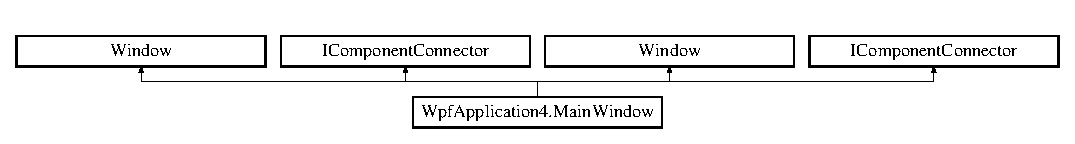
\includegraphics[height=1.489362cm]{classWpfApplication4_1_1MainWindow}
\end{center}
\end{figure}
\subsection*{Public Member Functions}
\begin{DoxyCompactItemize}
\item 
void \hyperlink{classWpfApplication4_1_1MainWindow_ab083c073f35c2d1f18b230aeef1c8a53}{Initialize\-Component} ()
\begin{DoxyCompactList}\small\item\em Initialize\-Component \end{DoxyCompactList}\item 
void \hyperlink{classWpfApplication4_1_1MainWindow_ab083c073f35c2d1f18b230aeef1c8a53}{Initialize\-Component} ()
\begin{DoxyCompactList}\small\item\em Initialize\-Component \end{DoxyCompactList}\end{DoxyCompactItemize}
\subsection*{Package Attributes}
\begin{DoxyCompactItemize}
\item 
System.\-Windows.\-Controls.\-Canvas \hyperlink{classWpfApplication4_1_1MainWindow_ad3ee7f5fe2642960f22f268f3c026990}{skeleton}
\item 
System.\-Windows.\-Controls.\-Label \hyperlink{classWpfApplication4_1_1MainWindow_a827708d162b3b2a34bf06a1c6ddc3b3d}{lbl\-Angel}
\item 
System.\-Windows.\-Controls.\-Text\-Box \hyperlink{classWpfApplication4_1_1MainWindow_a1c0b78db264ed19126b96830a5700bcd}{txt\-Joints}
\item 
System.\-Windows.\-Controls.\-Button \hyperlink{classWpfApplication4_1_1MainWindow_a8df403b3dd51676987f0f00b128cfa2b}{Start\-Recording}
\item 
System.\-Windows.\-Controls.\-Button \hyperlink{classWpfApplication4_1_1MainWindow_aab97058b3cbf0a1b083d1de7f011af39}{Start\-Replaying}
\end{DoxyCompactItemize}
\subsection*{Private Member Functions}
\begin{DoxyCompactItemize}
\item 
void \\*
System.\-Windows.\-Markup.\-I\-Component\-Connector. \hyperlink{classWpfApplication4_1_1MainWindow_aa918d7d7cc134fa18ca064739925be9a}{Connect} (int connection\-Id, object target)
\item 
void \\*
System.\-Windows.\-Markup.\-I\-Component\-Connector. \hyperlink{classWpfApplication4_1_1MainWindow_aa918d7d7cc134fa18ca064739925be9a}{Connect} (int connection\-Id, object target)
\end{DoxyCompactItemize}
\subsection*{Private Attributes}
\begin{DoxyCompactItemize}
\item 
bool \hyperlink{classWpfApplication4_1_1MainWindow_a39b4ae67911d755f5cccb22a5e80fe32}{\-\_\-content\-Loaded}
\end{DoxyCompactItemize}


\subsection{Detailed Description}
\hyperlink{classWpfApplication4_1_1MainWindow}{Main\-Window} 



\subsection{Member Function Documentation}
\hypertarget{classWpfApplication4_1_1MainWindow_aa918d7d7cc134fa18ca064739925be9a}{\index{Wpf\-Application4\-::\-Main\-Window@{Wpf\-Application4\-::\-Main\-Window}!Connect@{Connect}}
\index{Connect@{Connect}!WpfApplication4::MainWindow@{Wpf\-Application4\-::\-Main\-Window}}
\subsubsection[{Connect}]{\setlength{\rightskip}{0pt plus 5cm}void System.\-Windows.\-Markup.\-I\-Component\-Connector. Wpf\-Application4.\-Main\-Window.\-Connect (
\begin{DoxyParamCaption}
\item[{int}]{connection\-Id, }
\item[{object}]{target}
\end{DoxyParamCaption}
)\hspace{0.3cm}{\ttfamily [private]}}}\label{classWpfApplication4_1_1MainWindow_aa918d7d7cc134fa18ca064739925be9a}
\hypertarget{classWpfApplication4_1_1MainWindow_aa918d7d7cc134fa18ca064739925be9a}{\index{Wpf\-Application4\-::\-Main\-Window@{Wpf\-Application4\-::\-Main\-Window}!Connect@{Connect}}
\index{Connect@{Connect}!WpfApplication4::MainWindow@{Wpf\-Application4\-::\-Main\-Window}}
\subsubsection[{Connect}]{\setlength{\rightskip}{0pt plus 5cm}void System.\-Windows.\-Markup.\-I\-Component\-Connector. Wpf\-Application4.\-Main\-Window.\-Connect (
\begin{DoxyParamCaption}
\item[{int}]{connection\-Id, }
\item[{object}]{target}
\end{DoxyParamCaption}
)\hspace{0.3cm}{\ttfamily [private]}}}\label{classWpfApplication4_1_1MainWindow_aa918d7d7cc134fa18ca064739925be9a}
\hypertarget{classWpfApplication4_1_1MainWindow_ab083c073f35c2d1f18b230aeef1c8a53}{\index{Wpf\-Application4\-::\-Main\-Window@{Wpf\-Application4\-::\-Main\-Window}!Initialize\-Component@{Initialize\-Component}}
\index{Initialize\-Component@{Initialize\-Component}!WpfApplication4::MainWindow@{Wpf\-Application4\-::\-Main\-Window}}
\subsubsection[{Initialize\-Component}]{\setlength{\rightskip}{0pt plus 5cm}void Wpf\-Application4.\-Main\-Window.\-Initialize\-Component (
\begin{DoxyParamCaption}
{}
\end{DoxyParamCaption}
)}}\label{classWpfApplication4_1_1MainWindow_ab083c073f35c2d1f18b230aeef1c8a53}


Initialize\-Component 

\hypertarget{classWpfApplication4_1_1MainWindow_ab083c073f35c2d1f18b230aeef1c8a53}{\index{Wpf\-Application4\-::\-Main\-Window@{Wpf\-Application4\-::\-Main\-Window}!Initialize\-Component@{Initialize\-Component}}
\index{Initialize\-Component@{Initialize\-Component}!WpfApplication4::MainWindow@{Wpf\-Application4\-::\-Main\-Window}}
\subsubsection[{Initialize\-Component}]{\setlength{\rightskip}{0pt plus 5cm}void Wpf\-Application4.\-Main\-Window.\-Initialize\-Component (
\begin{DoxyParamCaption}
{}
\end{DoxyParamCaption}
)}}\label{classWpfApplication4_1_1MainWindow_ab083c073f35c2d1f18b230aeef1c8a53}


Initialize\-Component 



\subsection{Member Data Documentation}
\hypertarget{classWpfApplication4_1_1MainWindow_a39b4ae67911d755f5cccb22a5e80fe32}{\index{Wpf\-Application4\-::\-Main\-Window@{Wpf\-Application4\-::\-Main\-Window}!\-\_\-content\-Loaded@{\-\_\-content\-Loaded}}
\index{\-\_\-content\-Loaded@{\-\_\-content\-Loaded}!WpfApplication4::MainWindow@{Wpf\-Application4\-::\-Main\-Window}}
\subsubsection[{\-\_\-content\-Loaded}]{\setlength{\rightskip}{0pt plus 5cm}bool Wpf\-Application4.\-Main\-Window.\-\_\-content\-Loaded\hspace{0.3cm}{\ttfamily [private]}}}\label{classWpfApplication4_1_1MainWindow_a39b4ae67911d755f5cccb22a5e80fe32}
\hypertarget{classWpfApplication4_1_1MainWindow_a827708d162b3b2a34bf06a1c6ddc3b3d}{\index{Wpf\-Application4\-::\-Main\-Window@{Wpf\-Application4\-::\-Main\-Window}!lbl\-Angel@{lbl\-Angel}}
\index{lbl\-Angel@{lbl\-Angel}!WpfApplication4::MainWindow@{Wpf\-Application4\-::\-Main\-Window}}
\subsubsection[{lbl\-Angel}]{\setlength{\rightskip}{0pt plus 5cm}System Windows Controls Label Wpf\-Application4.\-Main\-Window.\-lbl\-Angel\hspace{0.3cm}{\ttfamily [package]}}}\label{classWpfApplication4_1_1MainWindow_a827708d162b3b2a34bf06a1c6ddc3b3d}
\hypertarget{classWpfApplication4_1_1MainWindow_ad3ee7f5fe2642960f22f268f3c026990}{\index{Wpf\-Application4\-::\-Main\-Window@{Wpf\-Application4\-::\-Main\-Window}!skeleton@{skeleton}}
\index{skeleton@{skeleton}!WpfApplication4::MainWindow@{Wpf\-Application4\-::\-Main\-Window}}
\subsubsection[{skeleton}]{\setlength{\rightskip}{0pt plus 5cm}System Windows Controls Canvas Wpf\-Application4.\-Main\-Window.\-skeleton\hspace{0.3cm}{\ttfamily [package]}}}\label{classWpfApplication4_1_1MainWindow_ad3ee7f5fe2642960f22f268f3c026990}
\hypertarget{classWpfApplication4_1_1MainWindow_a8df403b3dd51676987f0f00b128cfa2b}{\index{Wpf\-Application4\-::\-Main\-Window@{Wpf\-Application4\-::\-Main\-Window}!Start\-Recording@{Start\-Recording}}
\index{Start\-Recording@{Start\-Recording}!WpfApplication4::MainWindow@{Wpf\-Application4\-::\-Main\-Window}}
\subsubsection[{Start\-Recording}]{\setlength{\rightskip}{0pt plus 5cm}System.\-Windows.\-Controls.\-Button Wpf\-Application4.\-Main\-Window.\-Start\-Recording\hspace{0.3cm}{\ttfamily [package]}}}\label{classWpfApplication4_1_1MainWindow_a8df403b3dd51676987f0f00b128cfa2b}
\hypertarget{classWpfApplication4_1_1MainWindow_aab97058b3cbf0a1b083d1de7f011af39}{\index{Wpf\-Application4\-::\-Main\-Window@{Wpf\-Application4\-::\-Main\-Window}!Start\-Replaying@{Start\-Replaying}}
\index{Start\-Replaying@{Start\-Replaying}!WpfApplication4::MainWindow@{Wpf\-Application4\-::\-Main\-Window}}
\subsubsection[{Start\-Replaying}]{\setlength{\rightskip}{0pt plus 5cm}System.\-Windows.\-Controls.\-Button Wpf\-Application4.\-Main\-Window.\-Start\-Replaying\hspace{0.3cm}{\ttfamily [package]}}}\label{classWpfApplication4_1_1MainWindow_aab97058b3cbf0a1b083d1de7f011af39}
\hypertarget{classWpfApplication4_1_1MainWindow_a1c0b78db264ed19126b96830a5700bcd}{\index{Wpf\-Application4\-::\-Main\-Window@{Wpf\-Application4\-::\-Main\-Window}!txt\-Joints@{txt\-Joints}}
\index{txt\-Joints@{txt\-Joints}!WpfApplication4::MainWindow@{Wpf\-Application4\-::\-Main\-Window}}
\subsubsection[{txt\-Joints}]{\setlength{\rightskip}{0pt plus 5cm}System Windows Controls Text\-Box Wpf\-Application4.\-Main\-Window.\-txt\-Joints\hspace{0.3cm}{\ttfamily [package]}}}\label{classWpfApplication4_1_1MainWindow_a1c0b78db264ed19126b96830a5700bcd}


The documentation for this class was generated from the following files\-:\begin{DoxyCompactItemize}
\item 
obj/x86/\-Debug/\hyperlink{Debug_2MainWindow_8g_8cs}{Main\-Window.\-g.\-cs}\item 
obj/x86/\-Debug/\hyperlink{Debug_2MainWindow_8g_8i_8cs}{Main\-Window.\-g.\-i.\-cs}\end{DoxyCompactItemize}

\hypertarget{classUTKinectSkeletonMovementDetector_1_1MovementLogCtreationWorker}{\section{U\-T\-Kinect\-Skeleton\-Movement\-Detector.\-Movement\-Log\-Ctreation\-Worker Class Reference}
\label{classUTKinectSkeletonMovementDetector_1_1MovementLogCtreationWorker}\index{U\-T\-Kinect\-Skeleton\-Movement\-Detector.\-Movement\-Log\-Ctreation\-Worker@{U\-T\-Kinect\-Skeleton\-Movement\-Detector.\-Movement\-Log\-Ctreation\-Worker}}
}


movement log creation worker class  


\subsection*{Public Member Functions}
\begin{DoxyCompactItemize}
\item 
delegate void \hyperlink{classUTKinectSkeletonMovementDetector_1_1MovementLogCtreationWorker_a812bd166505941b61f4c4d33345bd1f5}{On\-Worker\-Method\-Complete\-Delegate} (string message)
\item 
\hyperlink{classUTKinectSkeletonMovementDetector_1_1MovementLogCtreationWorker_aff1e02f238a10168e4c24468911a37f0}{Movement\-Log\-Ctreation\-Worker} (List$<$ \hyperlink{classUTKinectSkeletonMovementDetector_1_1MySkeletonFrame}{My\-Skeleton\-Frame} $>$ sframes, string \hyperlink{classUTKinectSkeletonMovementDetector_1_1MovementLogCtreationWorker_ab8603c7df27474a6cac515572ffc2c92}{path})
\item 
void \hyperlink{classUTKinectSkeletonMovementDetector_1_1MovementLogCtreationWorker_a22e7b14a025767fd5bbe00e5e921fbb1}{Worker\-Method} ()
\begin{DoxyCompactList}\small\item\em main worker method \end{DoxyCompactList}\end{DoxyCompactItemize}
\subsection*{Events}
\begin{DoxyCompactItemize}
\item 
\hyperlink{classUTKinectSkeletonMovementDetector_1_1MovementLogCtreationWorker_a812bd166505941b61f4c4d33345bd1f5}{On\-Worker\-Method\-Complete\-Delegate} \hyperlink{classUTKinectSkeletonMovementDetector_1_1MovementLogCtreationWorker_a9602a7bd07fa4db7c977303e6b25e4ec}{On\-Worker\-Complete}
\end{DoxyCompactItemize}
\subsection*{Private Attributes}
\begin{DoxyCompactItemize}
\item 
List$<$ \hyperlink{classUTKinectSkeletonMovementDetector_1_1MySkeletonFrame}{My\-Skeleton\-Frame} $>$ \hyperlink{classUTKinectSkeletonMovementDetector_1_1MovementLogCtreationWorker_ae6904944298f18adcf91f40d438d1dea}{skeletonframes}
\item 
string \hyperlink{classUTKinectSkeletonMovementDetector_1_1MovementLogCtreationWorker_ab8603c7df27474a6cac515572ffc2c92}{path}
\end{DoxyCompactItemize}


\subsection{Detailed Description}
movement log creation worker class 



\subsection{Constructor \& Destructor Documentation}
\hypertarget{classUTKinectSkeletonMovementDetector_1_1MovementLogCtreationWorker_aff1e02f238a10168e4c24468911a37f0}{\index{U\-T\-Kinect\-Skeleton\-Movement\-Detector\-::\-Movement\-Log\-Ctreation\-Worker@{U\-T\-Kinect\-Skeleton\-Movement\-Detector\-::\-Movement\-Log\-Ctreation\-Worker}!Movement\-Log\-Ctreation\-Worker@{Movement\-Log\-Ctreation\-Worker}}
\index{Movement\-Log\-Ctreation\-Worker@{Movement\-Log\-Ctreation\-Worker}!UTKinectSkeletonMovementDetector::MovementLogCtreationWorker@{U\-T\-Kinect\-Skeleton\-Movement\-Detector\-::\-Movement\-Log\-Ctreation\-Worker}}
\subsubsection[{Movement\-Log\-Ctreation\-Worker}]{\setlength{\rightskip}{0pt plus 5cm}U\-T\-Kinect\-Skeleton\-Movement\-Detector.\-Movement\-Log\-Ctreation\-Worker.\-Movement\-Log\-Ctreation\-Worker (
\begin{DoxyParamCaption}
\item[{List$<$ {\bf My\-Skeleton\-Frame} $>$}]{sframes, }
\item[{string}]{path}
\end{DoxyParamCaption}
)}}\label{classUTKinectSkeletonMovementDetector_1_1MovementLogCtreationWorker_aff1e02f238a10168e4c24468911a37f0}


\subsection{Member Function Documentation}
\hypertarget{classUTKinectSkeletonMovementDetector_1_1MovementLogCtreationWorker_a812bd166505941b61f4c4d33345bd1f5}{\index{U\-T\-Kinect\-Skeleton\-Movement\-Detector\-::\-Movement\-Log\-Ctreation\-Worker@{U\-T\-Kinect\-Skeleton\-Movement\-Detector\-::\-Movement\-Log\-Ctreation\-Worker}!On\-Worker\-Method\-Complete\-Delegate@{On\-Worker\-Method\-Complete\-Delegate}}
\index{On\-Worker\-Method\-Complete\-Delegate@{On\-Worker\-Method\-Complete\-Delegate}!UTKinectSkeletonMovementDetector::MovementLogCtreationWorker@{U\-T\-Kinect\-Skeleton\-Movement\-Detector\-::\-Movement\-Log\-Ctreation\-Worker}}
\subsubsection[{On\-Worker\-Method\-Complete\-Delegate}]{\setlength{\rightskip}{0pt plus 5cm}delegate void U\-T\-Kinect\-Skeleton\-Movement\-Detector.\-Movement\-Log\-Ctreation\-Worker.\-On\-Worker\-Method\-Complete\-Delegate (
\begin{DoxyParamCaption}
\item[{string}]{message}
\end{DoxyParamCaption}
)}}\label{classUTKinectSkeletonMovementDetector_1_1MovementLogCtreationWorker_a812bd166505941b61f4c4d33345bd1f5}
\hypertarget{classUTKinectSkeletonMovementDetector_1_1MovementLogCtreationWorker_a22e7b14a025767fd5bbe00e5e921fbb1}{\index{U\-T\-Kinect\-Skeleton\-Movement\-Detector\-::\-Movement\-Log\-Ctreation\-Worker@{U\-T\-Kinect\-Skeleton\-Movement\-Detector\-::\-Movement\-Log\-Ctreation\-Worker}!Worker\-Method@{Worker\-Method}}
\index{Worker\-Method@{Worker\-Method}!UTKinectSkeletonMovementDetector::MovementLogCtreationWorker@{U\-T\-Kinect\-Skeleton\-Movement\-Detector\-::\-Movement\-Log\-Ctreation\-Worker}}
\subsubsection[{Worker\-Method}]{\setlength{\rightskip}{0pt plus 5cm}void U\-T\-Kinect\-Skeleton\-Movement\-Detector.\-Movement\-Log\-Ctreation\-Worker.\-Worker\-Method (
\begin{DoxyParamCaption}
{}
\end{DoxyParamCaption}
)}}\label{classUTKinectSkeletonMovementDetector_1_1MovementLogCtreationWorker_a22e7b14a025767fd5bbe00e5e921fbb1}


main worker method 



\subsection{Member Data Documentation}
\hypertarget{classUTKinectSkeletonMovementDetector_1_1MovementLogCtreationWorker_ab8603c7df27474a6cac515572ffc2c92}{\index{U\-T\-Kinect\-Skeleton\-Movement\-Detector\-::\-Movement\-Log\-Ctreation\-Worker@{U\-T\-Kinect\-Skeleton\-Movement\-Detector\-::\-Movement\-Log\-Ctreation\-Worker}!path@{path}}
\index{path@{path}!UTKinectSkeletonMovementDetector::MovementLogCtreationWorker@{U\-T\-Kinect\-Skeleton\-Movement\-Detector\-::\-Movement\-Log\-Ctreation\-Worker}}
\subsubsection[{path}]{\setlength{\rightskip}{0pt plus 5cm}string U\-T\-Kinect\-Skeleton\-Movement\-Detector.\-Movement\-Log\-Ctreation\-Worker.\-path\hspace{0.3cm}{\ttfamily [private]}}}\label{classUTKinectSkeletonMovementDetector_1_1MovementLogCtreationWorker_ab8603c7df27474a6cac515572ffc2c92}
\hypertarget{classUTKinectSkeletonMovementDetector_1_1MovementLogCtreationWorker_ae6904944298f18adcf91f40d438d1dea}{\index{U\-T\-Kinect\-Skeleton\-Movement\-Detector\-::\-Movement\-Log\-Ctreation\-Worker@{U\-T\-Kinect\-Skeleton\-Movement\-Detector\-::\-Movement\-Log\-Ctreation\-Worker}!skeletonframes@{skeletonframes}}
\index{skeletonframes@{skeletonframes}!UTKinectSkeletonMovementDetector::MovementLogCtreationWorker@{U\-T\-Kinect\-Skeleton\-Movement\-Detector\-::\-Movement\-Log\-Ctreation\-Worker}}
\subsubsection[{skeletonframes}]{\setlength{\rightskip}{0pt plus 5cm}List$<${\bf My\-Skeleton\-Frame}$>$ U\-T\-Kinect\-Skeleton\-Movement\-Detector.\-Movement\-Log\-Ctreation\-Worker.\-skeletonframes\hspace{0.3cm}{\ttfamily [private]}}}\label{classUTKinectSkeletonMovementDetector_1_1MovementLogCtreationWorker_ae6904944298f18adcf91f40d438d1dea}


\subsection{Event Documentation}
\hypertarget{classUTKinectSkeletonMovementDetector_1_1MovementLogCtreationWorker_a9602a7bd07fa4db7c977303e6b25e4ec}{\index{U\-T\-Kinect\-Skeleton\-Movement\-Detector\-::\-Movement\-Log\-Ctreation\-Worker@{U\-T\-Kinect\-Skeleton\-Movement\-Detector\-::\-Movement\-Log\-Ctreation\-Worker}!On\-Worker\-Complete@{On\-Worker\-Complete}}
\index{On\-Worker\-Complete@{On\-Worker\-Complete}!UTKinectSkeletonMovementDetector::MovementLogCtreationWorker@{U\-T\-Kinect\-Skeleton\-Movement\-Detector\-::\-Movement\-Log\-Ctreation\-Worker}}
\subsubsection[{On\-Worker\-Complete}]{\setlength{\rightskip}{0pt plus 5cm}{\bf On\-Worker\-Method\-Complete\-Delegate} U\-T\-Kinect\-Skeleton\-Movement\-Detector.\-Movement\-Log\-Ctreation\-Worker.\-On\-Worker\-Complete}}\label{classUTKinectSkeletonMovementDetector_1_1MovementLogCtreationWorker_a9602a7bd07fa4db7c977303e6b25e4ec}


The documentation for this class was generated from the following file\-:\begin{DoxyCompactItemize}
\item 
\hyperlink{MovementLogCtreationWorker_8cs}{Movement\-Log\-Ctreation\-Worker.\-cs}\end{DoxyCompactItemize}

\hypertarget{classUTKinectSkeletonMovementDetector_1_1MovieCreator}{\section{U\-T\-Kinect\-Skeleton\-Movement\-Detector.\-Movie\-Creator Class Reference}
\label{classUTKinectSkeletonMovementDetector_1_1MovieCreator}\index{U\-T\-Kinect\-Skeleton\-Movement\-Detector.\-Movie\-Creator@{U\-T\-Kinect\-Skeleton\-Movement\-Detector.\-Movie\-Creator}}
}
\subsection*{Static Public Member Functions}
\begin{DoxyCompactItemize}
\item 
static void \hyperlink{classUTKinectSkeletonMovementDetector_1_1MovieCreator_aafc8c8982e0970d2821bf25b0ce8e565}{create\-Skeleton\-Movie} (List$<$ \hyperlink{classUTKinectSkeletonMovementDetector_1_1MySkeletonFrame}{My\-Skeleton\-Frame} $>$ recorded\-\_\-skeleton\-\_\-frames, String path)
\item 
static void \hyperlink{classUTKinectSkeletonMovementDetector_1_1MovieCreator_a36477a3256e44e8b5d2ccf5f327ecfc5}{create\-Head\-Hided\-Movie} (List$<$ \hyperlink{classUTKinectSkeletonMovementDetector_1_1MyColorFrame}{My\-Color\-Frame} $>$ colorframes, List$<$ \hyperlink{classUTKinectSkeletonMovementDetector_1_1MySkeletonFrame}{My\-Skeleton\-Frame} $>$ skeletonframes, string path)
\item 
static void \hyperlink{classUTKinectSkeletonMovementDetector_1_1MovieCreator_a7fd66211d625f35e484a48f97c90f99d}{create\-Color\-Movie} (List$<$ \hyperlink{classUTKinectSkeletonMovementDetector_1_1MyColorFrame}{My\-Color\-Frame} $>$ recorded\-\_\-color\-\_\-frames, String path)
\item 
static void \hyperlink{classUTKinectSkeletonMovementDetector_1_1MovieCreator_a8d05c98c086701159a6741eba4b04b80}{create\-Overlay\-Movie} (ref List$<$ \hyperlink{classUTKinectSkeletonMovementDetector_1_1MyColorFrame}{My\-Color\-Frame} $>$ colorframes, ref List$<$ \hyperlink{classUTKinectSkeletonMovementDetector_1_1MySkeletonFrame}{My\-Skeleton\-Frame} $>$ skeletonframes, string path)
\end{DoxyCompactItemize}
\subsection*{Static Private Member Functions}
\begin{DoxyCompactItemize}
\item 
static void \hyperlink{classUTKinectSkeletonMovementDetector_1_1MovieCreator_aeffcfd490d691f74541c9426fb6eb2fe}{create\-Movie} (List$<$ System.\-Drawing.\-Bitmap $>$ images, String path)
\end{DoxyCompactItemize}


\subsection{Member Function Documentation}
\hypertarget{classUTKinectSkeletonMovementDetector_1_1MovieCreator_a7fd66211d625f35e484a48f97c90f99d}{\index{U\-T\-Kinect\-Skeleton\-Movement\-Detector\-::\-Movie\-Creator@{U\-T\-Kinect\-Skeleton\-Movement\-Detector\-::\-Movie\-Creator}!create\-Color\-Movie@{create\-Color\-Movie}}
\index{create\-Color\-Movie@{create\-Color\-Movie}!UTKinectSkeletonMovementDetector::MovieCreator@{U\-T\-Kinect\-Skeleton\-Movement\-Detector\-::\-Movie\-Creator}}
\subsubsection[{create\-Color\-Movie}]{\setlength{\rightskip}{0pt plus 5cm}static void U\-T\-Kinect\-Skeleton\-Movement\-Detector.\-Movie\-Creator.\-create\-Color\-Movie (
\begin{DoxyParamCaption}
\item[{List$<$ {\bf My\-Color\-Frame} $>$}]{recorded\-\_\-color\-\_\-frames, }
\item[{String}]{path}
\end{DoxyParamCaption}
)\hspace{0.3cm}{\ttfamily [static]}}}\label{classUTKinectSkeletonMovementDetector_1_1MovieCreator_a7fd66211d625f35e484a48f97c90f99d}
\hypertarget{classUTKinectSkeletonMovementDetector_1_1MovieCreator_a36477a3256e44e8b5d2ccf5f327ecfc5}{\index{U\-T\-Kinect\-Skeleton\-Movement\-Detector\-::\-Movie\-Creator@{U\-T\-Kinect\-Skeleton\-Movement\-Detector\-::\-Movie\-Creator}!create\-Head\-Hided\-Movie@{create\-Head\-Hided\-Movie}}
\index{create\-Head\-Hided\-Movie@{create\-Head\-Hided\-Movie}!UTKinectSkeletonMovementDetector::MovieCreator@{U\-T\-Kinect\-Skeleton\-Movement\-Detector\-::\-Movie\-Creator}}
\subsubsection[{create\-Head\-Hided\-Movie}]{\setlength{\rightskip}{0pt plus 5cm}static void U\-T\-Kinect\-Skeleton\-Movement\-Detector.\-Movie\-Creator.\-create\-Head\-Hided\-Movie (
\begin{DoxyParamCaption}
\item[{List$<$ {\bf My\-Color\-Frame} $>$}]{colorframes, }
\item[{List$<$ {\bf My\-Skeleton\-Frame} $>$}]{skeletonframes, }
\item[{string}]{path}
\end{DoxyParamCaption}
)\hspace{0.3cm}{\ttfamily [static]}}}\label{classUTKinectSkeletonMovementDetector_1_1MovieCreator_a36477a3256e44e8b5d2ccf5f327ecfc5}
\hypertarget{classUTKinectSkeletonMovementDetector_1_1MovieCreator_aeffcfd490d691f74541c9426fb6eb2fe}{\index{U\-T\-Kinect\-Skeleton\-Movement\-Detector\-::\-Movie\-Creator@{U\-T\-Kinect\-Skeleton\-Movement\-Detector\-::\-Movie\-Creator}!create\-Movie@{create\-Movie}}
\index{create\-Movie@{create\-Movie}!UTKinectSkeletonMovementDetector::MovieCreator@{U\-T\-Kinect\-Skeleton\-Movement\-Detector\-::\-Movie\-Creator}}
\subsubsection[{create\-Movie}]{\setlength{\rightskip}{0pt plus 5cm}static void U\-T\-Kinect\-Skeleton\-Movement\-Detector.\-Movie\-Creator.\-create\-Movie (
\begin{DoxyParamCaption}
\item[{List$<$ System.\-Drawing.\-Bitmap $>$}]{images, }
\item[{String}]{path}
\end{DoxyParamCaption}
)\hspace{0.3cm}{\ttfamily [static]}, {\ttfamily [private]}}}\label{classUTKinectSkeletonMovementDetector_1_1MovieCreator_aeffcfd490d691f74541c9426fb6eb2fe}
\hypertarget{classUTKinectSkeletonMovementDetector_1_1MovieCreator_a8d05c98c086701159a6741eba4b04b80}{\index{U\-T\-Kinect\-Skeleton\-Movement\-Detector\-::\-Movie\-Creator@{U\-T\-Kinect\-Skeleton\-Movement\-Detector\-::\-Movie\-Creator}!create\-Overlay\-Movie@{create\-Overlay\-Movie}}
\index{create\-Overlay\-Movie@{create\-Overlay\-Movie}!UTKinectSkeletonMovementDetector::MovieCreator@{U\-T\-Kinect\-Skeleton\-Movement\-Detector\-::\-Movie\-Creator}}
\subsubsection[{create\-Overlay\-Movie}]{\setlength{\rightskip}{0pt plus 5cm}static void U\-T\-Kinect\-Skeleton\-Movement\-Detector.\-Movie\-Creator.\-create\-Overlay\-Movie (
\begin{DoxyParamCaption}
\item[{ref List$<$ {\bf My\-Color\-Frame} $>$}]{colorframes, }
\item[{ref List$<$ {\bf My\-Skeleton\-Frame} $>$}]{skeletonframes, }
\item[{string}]{path}
\end{DoxyParamCaption}
)\hspace{0.3cm}{\ttfamily [static]}}}\label{classUTKinectSkeletonMovementDetector_1_1MovieCreator_a8d05c98c086701159a6741eba4b04b80}
\hypertarget{classUTKinectSkeletonMovementDetector_1_1MovieCreator_aafc8c8982e0970d2821bf25b0ce8e565}{\index{U\-T\-Kinect\-Skeleton\-Movement\-Detector\-::\-Movie\-Creator@{U\-T\-Kinect\-Skeleton\-Movement\-Detector\-::\-Movie\-Creator}!create\-Skeleton\-Movie@{create\-Skeleton\-Movie}}
\index{create\-Skeleton\-Movie@{create\-Skeleton\-Movie}!UTKinectSkeletonMovementDetector::MovieCreator@{U\-T\-Kinect\-Skeleton\-Movement\-Detector\-::\-Movie\-Creator}}
\subsubsection[{create\-Skeleton\-Movie}]{\setlength{\rightskip}{0pt plus 5cm}static void U\-T\-Kinect\-Skeleton\-Movement\-Detector.\-Movie\-Creator.\-create\-Skeleton\-Movie (
\begin{DoxyParamCaption}
\item[{List$<$ {\bf My\-Skeleton\-Frame} $>$}]{recorded\-\_\-skeleton\-\_\-frames, }
\item[{String}]{path}
\end{DoxyParamCaption}
)\hspace{0.3cm}{\ttfamily [static]}}}\label{classUTKinectSkeletonMovementDetector_1_1MovieCreator_aafc8c8982e0970d2821bf25b0ce8e565}


The documentation for this class was generated from the following file\-:\begin{DoxyCompactItemize}
\item 
\hyperlink{MovieCreator_8cs}{Movie\-Creator.\-cs}\end{DoxyCompactItemize}

\hypertarget{classUTKinectSkeletonMovementDetector_1_1MyColorFrame}{\section{U\-T\-Kinect\-Skeleton\-Movement\-Detector.\-My\-Color\-Frame Class Reference}
\label{classUTKinectSkeletonMovementDetector_1_1MyColorFrame}\index{U\-T\-Kinect\-Skeleton\-Movement\-Detector.\-My\-Color\-Frame@{U\-T\-Kinect\-Skeleton\-Movement\-Detector.\-My\-Color\-Frame}}
}
\subsection*{Public Member Functions}
\begin{DoxyCompactItemize}
\item 
\hyperlink{classUTKinectSkeletonMovementDetector_1_1MyColorFrame_a226964f4875f55245058c7980f59f035}{My\-Color\-Frame} (long \hyperlink{classUTKinectSkeletonMovementDetector_1_1MyColorFrame_af4cf6545d2ed2d17b72d585a09e055b4}{time\-Tag}, Bitmap colorbmp)
\item 
Memory\-Stream \hyperlink{classUTKinectSkeletonMovementDetector_1_1MyColorFrame_ad975d56f83d02fe22d3296960421df2a}{get\-Image\-Memory\-Stream} ()
\item 
long \hyperlink{classUTKinectSkeletonMovementDetector_1_1MyColorFrame_af72057adf889b56ee82ca052934f2507}{get\-Time} ()
\end{DoxyCompactItemize}
\subsection*{Private Attributes}
\begin{DoxyCompactItemize}
\item 
long \hyperlink{classUTKinectSkeletonMovementDetector_1_1MyColorFrame_af4cf6545d2ed2d17b72d585a09e055b4}{time\-Tag}
\item 
Memory\-Stream \hyperlink{classUTKinectSkeletonMovementDetector_1_1MyColorFrame_a380ba506814b7d4bc05b4cc47cca4b6b}{color\-Image\-Memory\-Stream}
\end{DoxyCompactItemize}


\subsection{Constructor \& Destructor Documentation}
\hypertarget{classUTKinectSkeletonMovementDetector_1_1MyColorFrame_a226964f4875f55245058c7980f59f035}{\index{U\-T\-Kinect\-Skeleton\-Movement\-Detector\-::\-My\-Color\-Frame@{U\-T\-Kinect\-Skeleton\-Movement\-Detector\-::\-My\-Color\-Frame}!My\-Color\-Frame@{My\-Color\-Frame}}
\index{My\-Color\-Frame@{My\-Color\-Frame}!UTKinectSkeletonMovementDetector::MyColorFrame@{U\-T\-Kinect\-Skeleton\-Movement\-Detector\-::\-My\-Color\-Frame}}
\subsubsection[{My\-Color\-Frame}]{\setlength{\rightskip}{0pt plus 5cm}U\-T\-Kinect\-Skeleton\-Movement\-Detector.\-My\-Color\-Frame.\-My\-Color\-Frame (
\begin{DoxyParamCaption}
\item[{long}]{time\-Tag, }
\item[{Bitmap}]{colorbmp}
\end{DoxyParamCaption}
)}}\label{classUTKinectSkeletonMovementDetector_1_1MyColorFrame_a226964f4875f55245058c7980f59f035}


\subsection{Member Function Documentation}
\hypertarget{classUTKinectSkeletonMovementDetector_1_1MyColorFrame_ad975d56f83d02fe22d3296960421df2a}{\index{U\-T\-Kinect\-Skeleton\-Movement\-Detector\-::\-My\-Color\-Frame@{U\-T\-Kinect\-Skeleton\-Movement\-Detector\-::\-My\-Color\-Frame}!get\-Image\-Memory\-Stream@{get\-Image\-Memory\-Stream}}
\index{get\-Image\-Memory\-Stream@{get\-Image\-Memory\-Stream}!UTKinectSkeletonMovementDetector::MyColorFrame@{U\-T\-Kinect\-Skeleton\-Movement\-Detector\-::\-My\-Color\-Frame}}
\subsubsection[{get\-Image\-Memory\-Stream}]{\setlength{\rightskip}{0pt plus 5cm}Memory\-Stream U\-T\-Kinect\-Skeleton\-Movement\-Detector.\-My\-Color\-Frame.\-get\-Image\-Memory\-Stream (
\begin{DoxyParamCaption}
{}
\end{DoxyParamCaption}
)}}\label{classUTKinectSkeletonMovementDetector_1_1MyColorFrame_ad975d56f83d02fe22d3296960421df2a}
\hypertarget{classUTKinectSkeletonMovementDetector_1_1MyColorFrame_af72057adf889b56ee82ca052934f2507}{\index{U\-T\-Kinect\-Skeleton\-Movement\-Detector\-::\-My\-Color\-Frame@{U\-T\-Kinect\-Skeleton\-Movement\-Detector\-::\-My\-Color\-Frame}!get\-Time@{get\-Time}}
\index{get\-Time@{get\-Time}!UTKinectSkeletonMovementDetector::MyColorFrame@{U\-T\-Kinect\-Skeleton\-Movement\-Detector\-::\-My\-Color\-Frame}}
\subsubsection[{get\-Time}]{\setlength{\rightskip}{0pt plus 5cm}long U\-T\-Kinect\-Skeleton\-Movement\-Detector.\-My\-Color\-Frame.\-get\-Time (
\begin{DoxyParamCaption}
{}
\end{DoxyParamCaption}
)}}\label{classUTKinectSkeletonMovementDetector_1_1MyColorFrame_af72057adf889b56ee82ca052934f2507}


\subsection{Member Data Documentation}
\hypertarget{classUTKinectSkeletonMovementDetector_1_1MyColorFrame_a380ba506814b7d4bc05b4cc47cca4b6b}{\index{U\-T\-Kinect\-Skeleton\-Movement\-Detector\-::\-My\-Color\-Frame@{U\-T\-Kinect\-Skeleton\-Movement\-Detector\-::\-My\-Color\-Frame}!color\-Image\-Memory\-Stream@{color\-Image\-Memory\-Stream}}
\index{color\-Image\-Memory\-Stream@{color\-Image\-Memory\-Stream}!UTKinectSkeletonMovementDetector::MyColorFrame@{U\-T\-Kinect\-Skeleton\-Movement\-Detector\-::\-My\-Color\-Frame}}
\subsubsection[{color\-Image\-Memory\-Stream}]{\setlength{\rightskip}{0pt plus 5cm}Memory\-Stream U\-T\-Kinect\-Skeleton\-Movement\-Detector.\-My\-Color\-Frame.\-color\-Image\-Memory\-Stream\hspace{0.3cm}{\ttfamily [private]}}}\label{classUTKinectSkeletonMovementDetector_1_1MyColorFrame_a380ba506814b7d4bc05b4cc47cca4b6b}
\hypertarget{classUTKinectSkeletonMovementDetector_1_1MyColorFrame_af4cf6545d2ed2d17b72d585a09e055b4}{\index{U\-T\-Kinect\-Skeleton\-Movement\-Detector\-::\-My\-Color\-Frame@{U\-T\-Kinect\-Skeleton\-Movement\-Detector\-::\-My\-Color\-Frame}!time\-Tag@{time\-Tag}}
\index{time\-Tag@{time\-Tag}!UTKinectSkeletonMovementDetector::MyColorFrame@{U\-T\-Kinect\-Skeleton\-Movement\-Detector\-::\-My\-Color\-Frame}}
\subsubsection[{time\-Tag}]{\setlength{\rightskip}{0pt plus 5cm}long U\-T\-Kinect\-Skeleton\-Movement\-Detector.\-My\-Color\-Frame.\-time\-Tag\hspace{0.3cm}{\ttfamily [private]}}}\label{classUTKinectSkeletonMovementDetector_1_1MyColorFrame_af4cf6545d2ed2d17b72d585a09e055b4}


The documentation for this class was generated from the following file\-:\begin{DoxyCompactItemize}
\item 
\hyperlink{MyColorFrame_8cs}{My\-Color\-Frame.\-cs}\end{DoxyCompactItemize}

\hypertarget{classUTKinectSkeletonMovementDetector_1_1MyOverlayFrame}{\section{U\-T\-Kinect\-Skeleton\-Movement\-Detector.\-My\-Overlay\-Frame Class Reference}
\label{classUTKinectSkeletonMovementDetector_1_1MyOverlayFrame}\index{U\-T\-Kinect\-Skeleton\-Movement\-Detector.\-My\-Overlay\-Frame@{U\-T\-Kinect\-Skeleton\-Movement\-Detector.\-My\-Overlay\-Frame}}
}
\subsection*{Public Member Functions}
\begin{DoxyCompactItemize}
\item 
\hyperlink{classUTKinectSkeletonMovementDetector_1_1MyOverlayFrame_a7852ef2ac2396d8a8ae3500ba44c13b3}{My\-Overlay\-Frame} (\hyperlink{classUTKinectSkeletonMovementDetector_1_1MySkeletonFrame}{My\-Skeleton\-Frame} skeletonframe, \hyperlink{classUTKinectSkeletonMovementDetector_1_1MyColorFrame}{My\-Color\-Frame} colorframe)
\item 
Memory\-Stream \hyperlink{classUTKinectSkeletonMovementDetector_1_1MyOverlayFrame_aa9b454d2c1418cf9039cdd066543c069}{get\-Overlay\-Memory\-Stream} ()
\item 
Memory\-Stream \hyperlink{classUTKinectSkeletonMovementDetector_1_1MyOverlayFrame_a7c9d73f006e7ecd7bfeece1ad78f2a64}{get\-Head\-Hided\-Memory\-Stream} ()
\end{DoxyCompactItemize}
\subsection*{Private Attributes}
\begin{DoxyCompactItemize}
\item 
long \hyperlink{classUTKinectSkeletonMovementDetector_1_1MyOverlayFrame_a45b8f233c8c84ef288dbc2f335bfd838}{timetag}
\item 
Memory\-Stream \hyperlink{classUTKinectSkeletonMovementDetector_1_1MyOverlayFrame_aee8d39380ccdb77dd048f711703dbff0}{overlay\-Memory\-Stream}
\item 
Memory\-Stream \hyperlink{classUTKinectSkeletonMovementDetector_1_1MyOverlayFrame_ab4852fb3c692907a96b9e23572094e38}{headhided\-Memory\-Stream}
\end{DoxyCompactItemize}


\subsection{Constructor \& Destructor Documentation}
\hypertarget{classUTKinectSkeletonMovementDetector_1_1MyOverlayFrame_a7852ef2ac2396d8a8ae3500ba44c13b3}{\index{U\-T\-Kinect\-Skeleton\-Movement\-Detector\-::\-My\-Overlay\-Frame@{U\-T\-Kinect\-Skeleton\-Movement\-Detector\-::\-My\-Overlay\-Frame}!My\-Overlay\-Frame@{My\-Overlay\-Frame}}
\index{My\-Overlay\-Frame@{My\-Overlay\-Frame}!UTKinectSkeletonMovementDetector::MyOverlayFrame@{U\-T\-Kinect\-Skeleton\-Movement\-Detector\-::\-My\-Overlay\-Frame}}
\subsubsection[{My\-Overlay\-Frame}]{\setlength{\rightskip}{0pt plus 5cm}U\-T\-Kinect\-Skeleton\-Movement\-Detector.\-My\-Overlay\-Frame.\-My\-Overlay\-Frame (
\begin{DoxyParamCaption}
\item[{{\bf My\-Skeleton\-Frame}}]{skeletonframe, }
\item[{{\bf My\-Color\-Frame}}]{colorframe}
\end{DoxyParamCaption}
)}}\label{classUTKinectSkeletonMovementDetector_1_1MyOverlayFrame_a7852ef2ac2396d8a8ae3500ba44c13b3}


\subsection{Member Function Documentation}
\hypertarget{classUTKinectSkeletonMovementDetector_1_1MyOverlayFrame_a7c9d73f006e7ecd7bfeece1ad78f2a64}{\index{U\-T\-Kinect\-Skeleton\-Movement\-Detector\-::\-My\-Overlay\-Frame@{U\-T\-Kinect\-Skeleton\-Movement\-Detector\-::\-My\-Overlay\-Frame}!get\-Head\-Hided\-Memory\-Stream@{get\-Head\-Hided\-Memory\-Stream}}
\index{get\-Head\-Hided\-Memory\-Stream@{get\-Head\-Hided\-Memory\-Stream}!UTKinectSkeletonMovementDetector::MyOverlayFrame@{U\-T\-Kinect\-Skeleton\-Movement\-Detector\-::\-My\-Overlay\-Frame}}
\subsubsection[{get\-Head\-Hided\-Memory\-Stream}]{\setlength{\rightskip}{0pt plus 5cm}Memory\-Stream U\-T\-Kinect\-Skeleton\-Movement\-Detector.\-My\-Overlay\-Frame.\-get\-Head\-Hided\-Memory\-Stream (
\begin{DoxyParamCaption}
{}
\end{DoxyParamCaption}
)}}\label{classUTKinectSkeletonMovementDetector_1_1MyOverlayFrame_a7c9d73f006e7ecd7bfeece1ad78f2a64}
\hypertarget{classUTKinectSkeletonMovementDetector_1_1MyOverlayFrame_aa9b454d2c1418cf9039cdd066543c069}{\index{U\-T\-Kinect\-Skeleton\-Movement\-Detector\-::\-My\-Overlay\-Frame@{U\-T\-Kinect\-Skeleton\-Movement\-Detector\-::\-My\-Overlay\-Frame}!get\-Overlay\-Memory\-Stream@{get\-Overlay\-Memory\-Stream}}
\index{get\-Overlay\-Memory\-Stream@{get\-Overlay\-Memory\-Stream}!UTKinectSkeletonMovementDetector::MyOverlayFrame@{U\-T\-Kinect\-Skeleton\-Movement\-Detector\-::\-My\-Overlay\-Frame}}
\subsubsection[{get\-Overlay\-Memory\-Stream}]{\setlength{\rightskip}{0pt plus 5cm}Memory\-Stream U\-T\-Kinect\-Skeleton\-Movement\-Detector.\-My\-Overlay\-Frame.\-get\-Overlay\-Memory\-Stream (
\begin{DoxyParamCaption}
{}
\end{DoxyParamCaption}
)}}\label{classUTKinectSkeletonMovementDetector_1_1MyOverlayFrame_aa9b454d2c1418cf9039cdd066543c069}


\subsection{Member Data Documentation}
\hypertarget{classUTKinectSkeletonMovementDetector_1_1MyOverlayFrame_ab4852fb3c692907a96b9e23572094e38}{\index{U\-T\-Kinect\-Skeleton\-Movement\-Detector\-::\-My\-Overlay\-Frame@{U\-T\-Kinect\-Skeleton\-Movement\-Detector\-::\-My\-Overlay\-Frame}!headhided\-Memory\-Stream@{headhided\-Memory\-Stream}}
\index{headhided\-Memory\-Stream@{headhided\-Memory\-Stream}!UTKinectSkeletonMovementDetector::MyOverlayFrame@{U\-T\-Kinect\-Skeleton\-Movement\-Detector\-::\-My\-Overlay\-Frame}}
\subsubsection[{headhided\-Memory\-Stream}]{\setlength{\rightskip}{0pt plus 5cm}Memory\-Stream U\-T\-Kinect\-Skeleton\-Movement\-Detector.\-My\-Overlay\-Frame.\-headhided\-Memory\-Stream\hspace{0.3cm}{\ttfamily [private]}}}\label{classUTKinectSkeletonMovementDetector_1_1MyOverlayFrame_ab4852fb3c692907a96b9e23572094e38}
\hypertarget{classUTKinectSkeletonMovementDetector_1_1MyOverlayFrame_aee8d39380ccdb77dd048f711703dbff0}{\index{U\-T\-Kinect\-Skeleton\-Movement\-Detector\-::\-My\-Overlay\-Frame@{U\-T\-Kinect\-Skeleton\-Movement\-Detector\-::\-My\-Overlay\-Frame}!overlay\-Memory\-Stream@{overlay\-Memory\-Stream}}
\index{overlay\-Memory\-Stream@{overlay\-Memory\-Stream}!UTKinectSkeletonMovementDetector::MyOverlayFrame@{U\-T\-Kinect\-Skeleton\-Movement\-Detector\-::\-My\-Overlay\-Frame}}
\subsubsection[{overlay\-Memory\-Stream}]{\setlength{\rightskip}{0pt plus 5cm}Memory\-Stream U\-T\-Kinect\-Skeleton\-Movement\-Detector.\-My\-Overlay\-Frame.\-overlay\-Memory\-Stream\hspace{0.3cm}{\ttfamily [private]}}}\label{classUTKinectSkeletonMovementDetector_1_1MyOverlayFrame_aee8d39380ccdb77dd048f711703dbff0}
\hypertarget{classUTKinectSkeletonMovementDetector_1_1MyOverlayFrame_a45b8f233c8c84ef288dbc2f335bfd838}{\index{U\-T\-Kinect\-Skeleton\-Movement\-Detector\-::\-My\-Overlay\-Frame@{U\-T\-Kinect\-Skeleton\-Movement\-Detector\-::\-My\-Overlay\-Frame}!timetag@{timetag}}
\index{timetag@{timetag}!UTKinectSkeletonMovementDetector::MyOverlayFrame@{U\-T\-Kinect\-Skeleton\-Movement\-Detector\-::\-My\-Overlay\-Frame}}
\subsubsection[{timetag}]{\setlength{\rightskip}{0pt plus 5cm}long U\-T\-Kinect\-Skeleton\-Movement\-Detector.\-My\-Overlay\-Frame.\-timetag\hspace{0.3cm}{\ttfamily [private]}}}\label{classUTKinectSkeletonMovementDetector_1_1MyOverlayFrame_a45b8f233c8c84ef288dbc2f335bfd838}


The documentation for this class was generated from the following file\-:\begin{DoxyCompactItemize}
\item 
\hyperlink{MyOverlayFrame_8cs}{My\-Overlay\-Frame.\-cs}\end{DoxyCompactItemize}

\hypertarget{classUTKinectSkeletonMovementDetector_1_1MySkeletonFrame}{\section{U\-T\-Kinect\-Skeleton\-Movement\-Detector.\-My\-Skeleton\-Frame Class Reference}
\label{classUTKinectSkeletonMovementDetector_1_1MySkeletonFrame}\index{U\-T\-Kinect\-Skeleton\-Movement\-Detector.\-My\-Skeleton\-Frame@{U\-T\-Kinect\-Skeleton\-Movement\-Detector.\-My\-Skeleton\-Frame}}
}


skeleton frame holder  


\subsection*{Public Member Functions}
\begin{DoxyCompactItemize}
\item 
\hyperlink{classUTKinectSkeletonMovementDetector_1_1MySkeletonFrame_a68103ea84830eb794d0ad718f9b6991a}{My\-Skeleton\-Frame} (Skeleton\mbox{[}$\,$\mbox{]} \hyperlink{classUTKinectSkeletonMovementDetector_1_1MySkeletonFrame_a0339c81d632197149363013284a46916}{skeletons}, long \hyperlink{classUTKinectSkeletonMovementDetector_1_1MySkeletonFrame_ab9d7e0d011a54cc036728ac94a2883b7}{time\-Tag})
\item 
void \hyperlink{classUTKinectSkeletonMovementDetector_1_1MySkeletonFrame_af3f9fc03eb13215e4305c572039aeb72}{save\-To\-File} (String path)
\item 
long \hyperlink{classUTKinectSkeletonMovementDetector_1_1MySkeletonFrame_a755f7df242e36e4e458b808d617cda4c}{get\-Time} ()
\item 
Memory\-Stream \hyperlink{classUTKinectSkeletonMovementDetector_1_1MySkeletonFrame_a61c75f59bce07a4925d21c55d4a12e01}{to\-Image\-Memory\-Stream} ()
\item 
Skeleton\mbox{[}$\,$\mbox{]} \hyperlink{classUTKinectSkeletonMovementDetector_1_1MySkeletonFrame_af88bf9afbf8f597fb6ed0087c100918d}{get\-Skeletons} ()
\end{DoxyCompactItemize}
\subsection*{Private Attributes}
\begin{DoxyCompactItemize}
\item 
long \hyperlink{classUTKinectSkeletonMovementDetector_1_1MySkeletonFrame_ab9d7e0d011a54cc036728ac94a2883b7}{time\-Tag}
\item 
Skeleton\mbox{[}$\,$\mbox{]} \hyperlink{classUTKinectSkeletonMovementDetector_1_1MySkeletonFrame_a0339c81d632197149363013284a46916}{skeletons}
\end{DoxyCompactItemize}


\subsection{Detailed Description}
skeleton frame holder 



\subsection{Constructor \& Destructor Documentation}
\hypertarget{classUTKinectSkeletonMovementDetector_1_1MySkeletonFrame_a68103ea84830eb794d0ad718f9b6991a}{\index{U\-T\-Kinect\-Skeleton\-Movement\-Detector\-::\-My\-Skeleton\-Frame@{U\-T\-Kinect\-Skeleton\-Movement\-Detector\-::\-My\-Skeleton\-Frame}!My\-Skeleton\-Frame@{My\-Skeleton\-Frame}}
\index{My\-Skeleton\-Frame@{My\-Skeleton\-Frame}!UTKinectSkeletonMovementDetector::MySkeletonFrame@{U\-T\-Kinect\-Skeleton\-Movement\-Detector\-::\-My\-Skeleton\-Frame}}
\subsubsection[{My\-Skeleton\-Frame}]{\setlength{\rightskip}{0pt plus 5cm}U\-T\-Kinect\-Skeleton\-Movement\-Detector.\-My\-Skeleton\-Frame.\-My\-Skeleton\-Frame (
\begin{DoxyParamCaption}
\item[{Skeleton\mbox{[}$\,$\mbox{]}}]{skeletons, }
\item[{long}]{time\-Tag}
\end{DoxyParamCaption}
)}}\label{classUTKinectSkeletonMovementDetector_1_1MySkeletonFrame_a68103ea84830eb794d0ad718f9b6991a}


\subsection{Member Function Documentation}
\hypertarget{classUTKinectSkeletonMovementDetector_1_1MySkeletonFrame_af88bf9afbf8f597fb6ed0087c100918d}{\index{U\-T\-Kinect\-Skeleton\-Movement\-Detector\-::\-My\-Skeleton\-Frame@{U\-T\-Kinect\-Skeleton\-Movement\-Detector\-::\-My\-Skeleton\-Frame}!get\-Skeletons@{get\-Skeletons}}
\index{get\-Skeletons@{get\-Skeletons}!UTKinectSkeletonMovementDetector::MySkeletonFrame@{U\-T\-Kinect\-Skeleton\-Movement\-Detector\-::\-My\-Skeleton\-Frame}}
\subsubsection[{get\-Skeletons}]{\setlength{\rightskip}{0pt plus 5cm}Skeleton \mbox{[}$\,$\mbox{]} U\-T\-Kinect\-Skeleton\-Movement\-Detector.\-My\-Skeleton\-Frame.\-get\-Skeletons (
\begin{DoxyParamCaption}
{}
\end{DoxyParamCaption}
)}}\label{classUTKinectSkeletonMovementDetector_1_1MySkeletonFrame_af88bf9afbf8f597fb6ed0087c100918d}
\hypertarget{classUTKinectSkeletonMovementDetector_1_1MySkeletonFrame_a755f7df242e36e4e458b808d617cda4c}{\index{U\-T\-Kinect\-Skeleton\-Movement\-Detector\-::\-My\-Skeleton\-Frame@{U\-T\-Kinect\-Skeleton\-Movement\-Detector\-::\-My\-Skeleton\-Frame}!get\-Time@{get\-Time}}
\index{get\-Time@{get\-Time}!UTKinectSkeletonMovementDetector::MySkeletonFrame@{U\-T\-Kinect\-Skeleton\-Movement\-Detector\-::\-My\-Skeleton\-Frame}}
\subsubsection[{get\-Time}]{\setlength{\rightskip}{0pt plus 5cm}long U\-T\-Kinect\-Skeleton\-Movement\-Detector.\-My\-Skeleton\-Frame.\-get\-Time (
\begin{DoxyParamCaption}
{}
\end{DoxyParamCaption}
)}}\label{classUTKinectSkeletonMovementDetector_1_1MySkeletonFrame_a755f7df242e36e4e458b808d617cda4c}
\hypertarget{classUTKinectSkeletonMovementDetector_1_1MySkeletonFrame_af3f9fc03eb13215e4305c572039aeb72}{\index{U\-T\-Kinect\-Skeleton\-Movement\-Detector\-::\-My\-Skeleton\-Frame@{U\-T\-Kinect\-Skeleton\-Movement\-Detector\-::\-My\-Skeleton\-Frame}!save\-To\-File@{save\-To\-File}}
\index{save\-To\-File@{save\-To\-File}!UTKinectSkeletonMovementDetector::MySkeletonFrame@{U\-T\-Kinect\-Skeleton\-Movement\-Detector\-::\-My\-Skeleton\-Frame}}
\subsubsection[{save\-To\-File}]{\setlength{\rightskip}{0pt plus 5cm}void U\-T\-Kinect\-Skeleton\-Movement\-Detector.\-My\-Skeleton\-Frame.\-save\-To\-File (
\begin{DoxyParamCaption}
\item[{String}]{path}
\end{DoxyParamCaption}
)}}\label{classUTKinectSkeletonMovementDetector_1_1MySkeletonFrame_af3f9fc03eb13215e4305c572039aeb72}
\hypertarget{classUTKinectSkeletonMovementDetector_1_1MySkeletonFrame_a61c75f59bce07a4925d21c55d4a12e01}{\index{U\-T\-Kinect\-Skeleton\-Movement\-Detector\-::\-My\-Skeleton\-Frame@{U\-T\-Kinect\-Skeleton\-Movement\-Detector\-::\-My\-Skeleton\-Frame}!to\-Image\-Memory\-Stream@{to\-Image\-Memory\-Stream}}
\index{to\-Image\-Memory\-Stream@{to\-Image\-Memory\-Stream}!UTKinectSkeletonMovementDetector::MySkeletonFrame@{U\-T\-Kinect\-Skeleton\-Movement\-Detector\-::\-My\-Skeleton\-Frame}}
\subsubsection[{to\-Image\-Memory\-Stream}]{\setlength{\rightskip}{0pt plus 5cm}Memory\-Stream U\-T\-Kinect\-Skeleton\-Movement\-Detector.\-My\-Skeleton\-Frame.\-to\-Image\-Memory\-Stream (
\begin{DoxyParamCaption}
{}
\end{DoxyParamCaption}
)}}\label{classUTKinectSkeletonMovementDetector_1_1MySkeletonFrame_a61c75f59bce07a4925d21c55d4a12e01}


\subsection{Member Data Documentation}
\hypertarget{classUTKinectSkeletonMovementDetector_1_1MySkeletonFrame_a0339c81d632197149363013284a46916}{\index{U\-T\-Kinect\-Skeleton\-Movement\-Detector\-::\-My\-Skeleton\-Frame@{U\-T\-Kinect\-Skeleton\-Movement\-Detector\-::\-My\-Skeleton\-Frame}!skeletons@{skeletons}}
\index{skeletons@{skeletons}!UTKinectSkeletonMovementDetector::MySkeletonFrame@{U\-T\-Kinect\-Skeleton\-Movement\-Detector\-::\-My\-Skeleton\-Frame}}
\subsubsection[{skeletons}]{\setlength{\rightskip}{0pt plus 5cm}Skeleton \mbox{[}$\,$\mbox{]} U\-T\-Kinect\-Skeleton\-Movement\-Detector.\-My\-Skeleton\-Frame.\-skeletons\hspace{0.3cm}{\ttfamily [private]}}}\label{classUTKinectSkeletonMovementDetector_1_1MySkeletonFrame_a0339c81d632197149363013284a46916}
\hypertarget{classUTKinectSkeletonMovementDetector_1_1MySkeletonFrame_ab9d7e0d011a54cc036728ac94a2883b7}{\index{U\-T\-Kinect\-Skeleton\-Movement\-Detector\-::\-My\-Skeleton\-Frame@{U\-T\-Kinect\-Skeleton\-Movement\-Detector\-::\-My\-Skeleton\-Frame}!time\-Tag@{time\-Tag}}
\index{time\-Tag@{time\-Tag}!UTKinectSkeletonMovementDetector::MySkeletonFrame@{U\-T\-Kinect\-Skeleton\-Movement\-Detector\-::\-My\-Skeleton\-Frame}}
\subsubsection[{time\-Tag}]{\setlength{\rightskip}{0pt plus 5cm}long U\-T\-Kinect\-Skeleton\-Movement\-Detector.\-My\-Skeleton\-Frame.\-time\-Tag\hspace{0.3cm}{\ttfamily [private]}}}\label{classUTKinectSkeletonMovementDetector_1_1MySkeletonFrame_ab9d7e0d011a54cc036728ac94a2883b7}


The documentation for this class was generated from the following file\-:\begin{DoxyCompactItemize}
\item 
\hyperlink{MySkeletonFrame_8cs}{My\-Skeleton\-Frame.\-cs}\end{DoxyCompactItemize}

\hypertarget{classWpfApplication4_1_1NameDialoge}{\section{Wpf\-Application4.\-Name\-Dialoge Class Reference}
\label{classWpfApplication4_1_1NameDialoge}\index{Wpf\-Application4.\-Name\-Dialoge@{Wpf\-Application4.\-Name\-Dialoge}}
}


\hyperlink{classWpfApplication4_1_1NameDialoge}{Name\-Dialoge}  


Inheritance diagram for Wpf\-Application4.\-Name\-Dialoge\-:\begin{figure}[H]
\begin{center}
\leavevmode
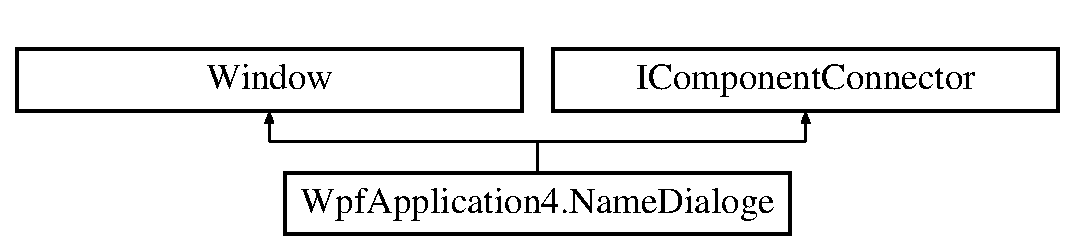
\includegraphics[height=2.000000cm]{classWpfApplication4_1_1NameDialoge}
\end{center}
\end{figure}
\subsection*{Public Member Functions}
\begin{DoxyCompactItemize}
\item 
void \hyperlink{classWpfApplication4_1_1NameDialoge_a32a6262c11e6072b01a17b18c5b0107a}{Initialize\-Component} ()
\begin{DoxyCompactList}\small\item\em Initialize\-Component \end{DoxyCompactList}\end{DoxyCompactItemize}
\subsection*{Package Attributes}
\begin{DoxyCompactItemize}
\item 
System.\-Windows.\-Controls.\-Button \hyperlink{classWpfApplication4_1_1NameDialoge_a66734ab0766d633159da4b222fb5914d}{ok\-\_\-button}
\item 
System.\-Windows.\-Controls.\-Button \hyperlink{classWpfApplication4_1_1NameDialoge_a159e41148753b8f8569224df378664f0}{cancel\-\_\-button}
\item 
System.\-Windows.\-Controls.\-Text\-Box \hyperlink{classWpfApplication4_1_1NameDialoge_a9cc6d5b5dfd140e835e30b6abd20f629}{name\-\_\-textbox}
\end{DoxyCompactItemize}
\subsection*{Private Member Functions}
\begin{DoxyCompactItemize}
\item 
void \\*
System.\-Windows.\-Markup.\-I\-Component\-Connector. \hyperlink{classWpfApplication4_1_1NameDialoge_abd3d69dc9ddc0781f2fe9f31b8331de4}{Connect} (int connection\-Id, object target)
\end{DoxyCompactItemize}
\subsection*{Private Attributes}
\begin{DoxyCompactItemize}
\item 
bool \hyperlink{classWpfApplication4_1_1NameDialoge_ad215f27c234ccc67665ebfb168138fa2}{\-\_\-content\-Loaded}
\end{DoxyCompactItemize}


\subsection{Detailed Description}
\hyperlink{classWpfApplication4_1_1NameDialoge}{Name\-Dialoge} 



\subsection{Member Function Documentation}
\hypertarget{classWpfApplication4_1_1NameDialoge_abd3d69dc9ddc0781f2fe9f31b8331de4}{\index{Wpf\-Application4\-::\-Name\-Dialoge@{Wpf\-Application4\-::\-Name\-Dialoge}!Connect@{Connect}}
\index{Connect@{Connect}!WpfApplication4::NameDialoge@{Wpf\-Application4\-::\-Name\-Dialoge}}
\subsubsection[{Connect}]{\setlength{\rightskip}{0pt plus 5cm}void System.\-Windows.\-Markup.\-I\-Component\-Connector. Wpf\-Application4.\-Name\-Dialoge.\-Connect (
\begin{DoxyParamCaption}
\item[{int}]{connection\-Id, }
\item[{object}]{target}
\end{DoxyParamCaption}
)\hspace{0.3cm}{\ttfamily [private]}}}\label{classWpfApplication4_1_1NameDialoge_abd3d69dc9ddc0781f2fe9f31b8331de4}
\hypertarget{classWpfApplication4_1_1NameDialoge_a32a6262c11e6072b01a17b18c5b0107a}{\index{Wpf\-Application4\-::\-Name\-Dialoge@{Wpf\-Application4\-::\-Name\-Dialoge}!Initialize\-Component@{Initialize\-Component}}
\index{Initialize\-Component@{Initialize\-Component}!WpfApplication4::NameDialoge@{Wpf\-Application4\-::\-Name\-Dialoge}}
\subsubsection[{Initialize\-Component}]{\setlength{\rightskip}{0pt plus 5cm}void Wpf\-Application4.\-Name\-Dialoge.\-Initialize\-Component (
\begin{DoxyParamCaption}
{}
\end{DoxyParamCaption}
)}}\label{classWpfApplication4_1_1NameDialoge_a32a6262c11e6072b01a17b18c5b0107a}


Initialize\-Component 



\subsection{Member Data Documentation}
\hypertarget{classWpfApplication4_1_1NameDialoge_ad215f27c234ccc67665ebfb168138fa2}{\index{Wpf\-Application4\-::\-Name\-Dialoge@{Wpf\-Application4\-::\-Name\-Dialoge}!\-\_\-content\-Loaded@{\-\_\-content\-Loaded}}
\index{\-\_\-content\-Loaded@{\-\_\-content\-Loaded}!WpfApplication4::NameDialoge@{Wpf\-Application4\-::\-Name\-Dialoge}}
\subsubsection[{\-\_\-content\-Loaded}]{\setlength{\rightskip}{0pt plus 5cm}bool Wpf\-Application4.\-Name\-Dialoge.\-\_\-content\-Loaded\hspace{0.3cm}{\ttfamily [private]}}}\label{classWpfApplication4_1_1NameDialoge_ad215f27c234ccc67665ebfb168138fa2}
\hypertarget{classWpfApplication4_1_1NameDialoge_a159e41148753b8f8569224df378664f0}{\index{Wpf\-Application4\-::\-Name\-Dialoge@{Wpf\-Application4\-::\-Name\-Dialoge}!cancel\-\_\-button@{cancel\-\_\-button}}
\index{cancel\-\_\-button@{cancel\-\_\-button}!WpfApplication4::NameDialoge@{Wpf\-Application4\-::\-Name\-Dialoge}}
\subsubsection[{cancel\-\_\-button}]{\setlength{\rightskip}{0pt plus 5cm}System.\-Windows.\-Controls.\-Button Wpf\-Application4.\-Name\-Dialoge.\-cancel\-\_\-button\hspace{0.3cm}{\ttfamily [package]}}}\label{classWpfApplication4_1_1NameDialoge_a159e41148753b8f8569224df378664f0}
\hypertarget{classWpfApplication4_1_1NameDialoge_a9cc6d5b5dfd140e835e30b6abd20f629}{\index{Wpf\-Application4\-::\-Name\-Dialoge@{Wpf\-Application4\-::\-Name\-Dialoge}!name\-\_\-textbox@{name\-\_\-textbox}}
\index{name\-\_\-textbox@{name\-\_\-textbox}!WpfApplication4::NameDialoge@{Wpf\-Application4\-::\-Name\-Dialoge}}
\subsubsection[{name\-\_\-textbox}]{\setlength{\rightskip}{0pt plus 5cm}System.\-Windows.\-Controls.\-Text\-Box Wpf\-Application4.\-Name\-Dialoge.\-name\-\_\-textbox\hspace{0.3cm}{\ttfamily [package]}}}\label{classWpfApplication4_1_1NameDialoge_a9cc6d5b5dfd140e835e30b6abd20f629}
\hypertarget{classWpfApplication4_1_1NameDialoge_a66734ab0766d633159da4b222fb5914d}{\index{Wpf\-Application4\-::\-Name\-Dialoge@{Wpf\-Application4\-::\-Name\-Dialoge}!ok\-\_\-button@{ok\-\_\-button}}
\index{ok\-\_\-button@{ok\-\_\-button}!WpfApplication4::NameDialoge@{Wpf\-Application4\-::\-Name\-Dialoge}}
\subsubsection[{ok\-\_\-button}]{\setlength{\rightskip}{0pt plus 5cm}System.\-Windows.\-Controls.\-Button Wpf\-Application4.\-Name\-Dialoge.\-ok\-\_\-button\hspace{0.3cm}{\ttfamily [package]}}}\label{classWpfApplication4_1_1NameDialoge_a66734ab0766d633159da4b222fb5914d}


The documentation for this class was generated from the following file\-:\begin{DoxyCompactItemize}
\item 
obj/x86/\-Release/\hyperlink{NameDialoge_8g_8i_8cs}{Name\-Dialoge.\-g.\-i.\-cs}\end{DoxyCompactItemize}

\hypertarget{classUTKinectSkeletonMovementDetector_1_1OverlayMovieCreatorWorker}{\section{U\-T\-Kinect\-Skeleton\-Movement\-Detector.\-Overlay\-Movie\-Creator\-Worker Class Reference}
\label{classUTKinectSkeletonMovementDetector_1_1OverlayMovieCreatorWorker}\index{U\-T\-Kinect\-Skeleton\-Movement\-Detector.\-Overlay\-Movie\-Creator\-Worker@{U\-T\-Kinect\-Skeleton\-Movement\-Detector.\-Overlay\-Movie\-Creator\-Worker}}
}


overlay movie creation worker class  


\subsection*{Public Member Functions}
\begin{DoxyCompactItemize}
\item 
delegate void \hyperlink{classUTKinectSkeletonMovementDetector_1_1OverlayMovieCreatorWorker_a8f0c6db2f98bfa154472f03a57f57965}{On\-Worker\-Method\-Complete\-Delegate} (string message)
\item 
\hyperlink{classUTKinectSkeletonMovementDetector_1_1OverlayMovieCreatorWorker_a3bd9c053c3557b128d9eddfd5661662e}{Overlay\-Movie\-Creator\-Worker} (ref List$<$ \hyperlink{classUTKinectSkeletonMovementDetector_1_1MyColorFrame}{My\-Color\-Frame} $>$ cframes, ref List$<$ \hyperlink{classUTKinectSkeletonMovementDetector_1_1MySkeletonFrame}{My\-Skeleton\-Frame} $>$ sframes, string \hyperlink{classUTKinectSkeletonMovementDetector_1_1OverlayMovieCreatorWorker_aea3e1a17daf934d675f8bdc54b08bb3a}{path})
\item 
void \hyperlink{classUTKinectSkeletonMovementDetector_1_1OverlayMovieCreatorWorker_aebd9b99b693ca67fc6d58e68828899dd}{Worker\-Method} ()
\begin{DoxyCompactList}\small\item\em main worker method \end{DoxyCompactList}\end{DoxyCompactItemize}
\subsection*{Events}
\begin{DoxyCompactItemize}
\item 
\hyperlink{classUTKinectSkeletonMovementDetector_1_1OverlayMovieCreatorWorker_a8f0c6db2f98bfa154472f03a57f57965}{On\-Worker\-Method\-Complete\-Delegate} \hyperlink{classUTKinectSkeletonMovementDetector_1_1OverlayMovieCreatorWorker_a8287ec8e540ee2d64881ae833d70df20}{On\-Worker\-Complete}
\end{DoxyCompactItemize}
\subsection*{Private Attributes}
\begin{DoxyCompactItemize}
\item 
List$<$ \hyperlink{classUTKinectSkeletonMovementDetector_1_1MyColorFrame}{My\-Color\-Frame} $>$ \hyperlink{classUTKinectSkeletonMovementDetector_1_1OverlayMovieCreatorWorker_a588f1618fadac569471f04d8e2e5f848}{colorframes}
\item 
List$<$ \hyperlink{classUTKinectSkeletonMovementDetector_1_1MySkeletonFrame}{My\-Skeleton\-Frame} $>$ \hyperlink{classUTKinectSkeletonMovementDetector_1_1OverlayMovieCreatorWorker_a98a89d8c89465db5bda6eea62d3b2bbb}{skeletonframes}
\item 
string \hyperlink{classUTKinectSkeletonMovementDetector_1_1OverlayMovieCreatorWorker_aea3e1a17daf934d675f8bdc54b08bb3a}{path}
\end{DoxyCompactItemize}


\subsection{Detailed Description}
overlay movie creation worker class 



\subsection{Constructor \& Destructor Documentation}
\hypertarget{classUTKinectSkeletonMovementDetector_1_1OverlayMovieCreatorWorker_a3bd9c053c3557b128d9eddfd5661662e}{\index{U\-T\-Kinect\-Skeleton\-Movement\-Detector\-::\-Overlay\-Movie\-Creator\-Worker@{U\-T\-Kinect\-Skeleton\-Movement\-Detector\-::\-Overlay\-Movie\-Creator\-Worker}!Overlay\-Movie\-Creator\-Worker@{Overlay\-Movie\-Creator\-Worker}}
\index{Overlay\-Movie\-Creator\-Worker@{Overlay\-Movie\-Creator\-Worker}!UTKinectSkeletonMovementDetector::OverlayMovieCreatorWorker@{U\-T\-Kinect\-Skeleton\-Movement\-Detector\-::\-Overlay\-Movie\-Creator\-Worker}}
\subsubsection[{Overlay\-Movie\-Creator\-Worker}]{\setlength{\rightskip}{0pt plus 5cm}U\-T\-Kinect\-Skeleton\-Movement\-Detector.\-Overlay\-Movie\-Creator\-Worker.\-Overlay\-Movie\-Creator\-Worker (
\begin{DoxyParamCaption}
\item[{ref List$<$ {\bf My\-Color\-Frame} $>$}]{cframes, }
\item[{ref List$<$ {\bf My\-Skeleton\-Frame} $>$}]{sframes, }
\item[{string}]{path}
\end{DoxyParamCaption}
)}}\label{classUTKinectSkeletonMovementDetector_1_1OverlayMovieCreatorWorker_a3bd9c053c3557b128d9eddfd5661662e}


\subsection{Member Function Documentation}
\hypertarget{classUTKinectSkeletonMovementDetector_1_1OverlayMovieCreatorWorker_a8f0c6db2f98bfa154472f03a57f57965}{\index{U\-T\-Kinect\-Skeleton\-Movement\-Detector\-::\-Overlay\-Movie\-Creator\-Worker@{U\-T\-Kinect\-Skeleton\-Movement\-Detector\-::\-Overlay\-Movie\-Creator\-Worker}!On\-Worker\-Method\-Complete\-Delegate@{On\-Worker\-Method\-Complete\-Delegate}}
\index{On\-Worker\-Method\-Complete\-Delegate@{On\-Worker\-Method\-Complete\-Delegate}!UTKinectSkeletonMovementDetector::OverlayMovieCreatorWorker@{U\-T\-Kinect\-Skeleton\-Movement\-Detector\-::\-Overlay\-Movie\-Creator\-Worker}}
\subsubsection[{On\-Worker\-Method\-Complete\-Delegate}]{\setlength{\rightskip}{0pt plus 5cm}delegate void U\-T\-Kinect\-Skeleton\-Movement\-Detector.\-Overlay\-Movie\-Creator\-Worker.\-On\-Worker\-Method\-Complete\-Delegate (
\begin{DoxyParamCaption}
\item[{string}]{message}
\end{DoxyParamCaption}
)}}\label{classUTKinectSkeletonMovementDetector_1_1OverlayMovieCreatorWorker_a8f0c6db2f98bfa154472f03a57f57965}
\hypertarget{classUTKinectSkeletonMovementDetector_1_1OverlayMovieCreatorWorker_aebd9b99b693ca67fc6d58e68828899dd}{\index{U\-T\-Kinect\-Skeleton\-Movement\-Detector\-::\-Overlay\-Movie\-Creator\-Worker@{U\-T\-Kinect\-Skeleton\-Movement\-Detector\-::\-Overlay\-Movie\-Creator\-Worker}!Worker\-Method@{Worker\-Method}}
\index{Worker\-Method@{Worker\-Method}!UTKinectSkeletonMovementDetector::OverlayMovieCreatorWorker@{U\-T\-Kinect\-Skeleton\-Movement\-Detector\-::\-Overlay\-Movie\-Creator\-Worker}}
\subsubsection[{Worker\-Method}]{\setlength{\rightskip}{0pt plus 5cm}void U\-T\-Kinect\-Skeleton\-Movement\-Detector.\-Overlay\-Movie\-Creator\-Worker.\-Worker\-Method (
\begin{DoxyParamCaption}
{}
\end{DoxyParamCaption}
)}}\label{classUTKinectSkeletonMovementDetector_1_1OverlayMovieCreatorWorker_aebd9b99b693ca67fc6d58e68828899dd}


main worker method 



\subsection{Member Data Documentation}
\hypertarget{classUTKinectSkeletonMovementDetector_1_1OverlayMovieCreatorWorker_a588f1618fadac569471f04d8e2e5f848}{\index{U\-T\-Kinect\-Skeleton\-Movement\-Detector\-::\-Overlay\-Movie\-Creator\-Worker@{U\-T\-Kinect\-Skeleton\-Movement\-Detector\-::\-Overlay\-Movie\-Creator\-Worker}!colorframes@{colorframes}}
\index{colorframes@{colorframes}!UTKinectSkeletonMovementDetector::OverlayMovieCreatorWorker@{U\-T\-Kinect\-Skeleton\-Movement\-Detector\-::\-Overlay\-Movie\-Creator\-Worker}}
\subsubsection[{colorframes}]{\setlength{\rightskip}{0pt plus 5cm}List$<${\bf My\-Color\-Frame}$>$ U\-T\-Kinect\-Skeleton\-Movement\-Detector.\-Overlay\-Movie\-Creator\-Worker.\-colorframes\hspace{0.3cm}{\ttfamily [private]}}}\label{classUTKinectSkeletonMovementDetector_1_1OverlayMovieCreatorWorker_a588f1618fadac569471f04d8e2e5f848}
\hypertarget{classUTKinectSkeletonMovementDetector_1_1OverlayMovieCreatorWorker_aea3e1a17daf934d675f8bdc54b08bb3a}{\index{U\-T\-Kinect\-Skeleton\-Movement\-Detector\-::\-Overlay\-Movie\-Creator\-Worker@{U\-T\-Kinect\-Skeleton\-Movement\-Detector\-::\-Overlay\-Movie\-Creator\-Worker}!path@{path}}
\index{path@{path}!UTKinectSkeletonMovementDetector::OverlayMovieCreatorWorker@{U\-T\-Kinect\-Skeleton\-Movement\-Detector\-::\-Overlay\-Movie\-Creator\-Worker}}
\subsubsection[{path}]{\setlength{\rightskip}{0pt plus 5cm}string U\-T\-Kinect\-Skeleton\-Movement\-Detector.\-Overlay\-Movie\-Creator\-Worker.\-path\hspace{0.3cm}{\ttfamily [private]}}}\label{classUTKinectSkeletonMovementDetector_1_1OverlayMovieCreatorWorker_aea3e1a17daf934d675f8bdc54b08bb3a}
\hypertarget{classUTKinectSkeletonMovementDetector_1_1OverlayMovieCreatorWorker_a98a89d8c89465db5bda6eea62d3b2bbb}{\index{U\-T\-Kinect\-Skeleton\-Movement\-Detector\-::\-Overlay\-Movie\-Creator\-Worker@{U\-T\-Kinect\-Skeleton\-Movement\-Detector\-::\-Overlay\-Movie\-Creator\-Worker}!skeletonframes@{skeletonframes}}
\index{skeletonframes@{skeletonframes}!UTKinectSkeletonMovementDetector::OverlayMovieCreatorWorker@{U\-T\-Kinect\-Skeleton\-Movement\-Detector\-::\-Overlay\-Movie\-Creator\-Worker}}
\subsubsection[{skeletonframes}]{\setlength{\rightskip}{0pt plus 5cm}List$<${\bf My\-Skeleton\-Frame}$>$ U\-T\-Kinect\-Skeleton\-Movement\-Detector.\-Overlay\-Movie\-Creator\-Worker.\-skeletonframes\hspace{0.3cm}{\ttfamily [private]}}}\label{classUTKinectSkeletonMovementDetector_1_1OverlayMovieCreatorWorker_a98a89d8c89465db5bda6eea62d3b2bbb}


\subsection{Event Documentation}
\hypertarget{classUTKinectSkeletonMovementDetector_1_1OverlayMovieCreatorWorker_a8287ec8e540ee2d64881ae833d70df20}{\index{U\-T\-Kinect\-Skeleton\-Movement\-Detector\-::\-Overlay\-Movie\-Creator\-Worker@{U\-T\-Kinect\-Skeleton\-Movement\-Detector\-::\-Overlay\-Movie\-Creator\-Worker}!On\-Worker\-Complete@{On\-Worker\-Complete}}
\index{On\-Worker\-Complete@{On\-Worker\-Complete}!UTKinectSkeletonMovementDetector::OverlayMovieCreatorWorker@{U\-T\-Kinect\-Skeleton\-Movement\-Detector\-::\-Overlay\-Movie\-Creator\-Worker}}
\subsubsection[{On\-Worker\-Complete}]{\setlength{\rightskip}{0pt plus 5cm}{\bf On\-Worker\-Method\-Complete\-Delegate} U\-T\-Kinect\-Skeleton\-Movement\-Detector.\-Overlay\-Movie\-Creator\-Worker.\-On\-Worker\-Complete}}\label{classUTKinectSkeletonMovementDetector_1_1OverlayMovieCreatorWorker_a8287ec8e540ee2d64881ae833d70df20}


The documentation for this class was generated from the following file\-:\begin{DoxyCompactItemize}
\item 
\hyperlink{OverlayMovieCreatorWorker_8cs}{Overlay\-Movie\-Creator\-Worker.\-cs}\end{DoxyCompactItemize}

\hypertarget{classUTKinectSkeletonMovementDetector_1_1progressDialog}{\section{U\-T\-Kinect\-Skeleton\-Movement\-Detector.\-progress\-Dialog Class Reference}
\label{classUTKinectSkeletonMovementDetector_1_1progressDialog}\index{U\-T\-Kinect\-Skeleton\-Movement\-Detector.\-progress\-Dialog@{U\-T\-Kinect\-Skeleton\-Movement\-Detector.\-progress\-Dialog}}
}


\hyperlink{classUTKinectSkeletonMovementDetector_1_1progressDialog}{progress\-Dialog}  


Inheritance diagram for U\-T\-Kinect\-Skeleton\-Movement\-Detector.\-progress\-Dialog\-:\begin{figure}[H]
\begin{center}
\leavevmode
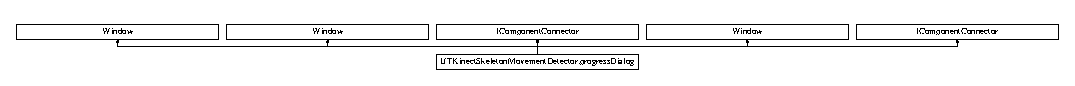
\includegraphics[height=0.713376cm]{classUTKinectSkeletonMovementDetector_1_1progressDialog}
\end{center}
\end{figure}
\subsection*{Public Member Functions}
\begin{DoxyCompactItemize}
\item 
void \hyperlink{classUTKinectSkeletonMovementDetector_1_1progressDialog_ad67bc7d8762e3496e8d812bdea3946ff}{Initialize\-Component} ()
\begin{DoxyCompactList}\small\item\em Initialize\-Component \end{DoxyCompactList}\item 
void \hyperlink{classUTKinectSkeletonMovementDetector_1_1progressDialog_ad67bc7d8762e3496e8d812bdea3946ff}{Initialize\-Component} ()
\begin{DoxyCompactList}\small\item\em Initialize\-Component \end{DoxyCompactList}\item 
\hyperlink{classUTKinectSkeletonMovementDetector_1_1progressDialog_ab99cb0504b3fb6d18cedcaa82c627f4c}{progress\-Dialog} (string msg)
\end{DoxyCompactItemize}
\subsection*{Package Attributes}
\begin{DoxyCompactItemize}
\item 
System.\-Windows.\-Controls.\-Label \hyperlink{classUTKinectSkeletonMovementDetector_1_1progressDialog_a34d8fd1e77c9e7cbc95fc31afd0223c1}{label}
\item 
System.\-Windows.\-Controls.\-Progress\-Bar \hyperlink{classUTKinectSkeletonMovementDetector_1_1progressDialog_a4c26b817c4d2e43742f7fce7c300fe73}{filmprogress}
\end{DoxyCompactItemize}
\subsection*{Private Member Functions}
\begin{DoxyCompactItemize}
\item 
void \\*
System.\-Windows.\-Markup.\-I\-Component\-Connector. \hyperlink{classUTKinectSkeletonMovementDetector_1_1progressDialog_a86f10eb726b9c254e295b998fc9cde94}{Connect} (int connection\-Id, object target)
\item 
void \\*
System.\-Windows.\-Markup.\-I\-Component\-Connector. \hyperlink{classUTKinectSkeletonMovementDetector_1_1progressDialog_a86f10eb726b9c254e295b998fc9cde94}{Connect} (int connection\-Id, object target)
\end{DoxyCompactItemize}
\subsection*{Private Attributes}
\begin{DoxyCompactItemize}
\item 
bool \hyperlink{classUTKinectSkeletonMovementDetector_1_1progressDialog_a08d8f7d167f4b804d017995e6ec978e2}{\-\_\-content\-Loaded}
\end{DoxyCompactItemize}


\subsection{Detailed Description}
\hyperlink{classUTKinectSkeletonMovementDetector_1_1progressDialog}{progress\-Dialog} 

Interaction logic for progress\-Dialog.\-xaml 

\subsection{Constructor \& Destructor Documentation}
\hypertarget{classUTKinectSkeletonMovementDetector_1_1progressDialog_ab99cb0504b3fb6d18cedcaa82c627f4c}{\index{U\-T\-Kinect\-Skeleton\-Movement\-Detector\-::progress\-Dialog@{U\-T\-Kinect\-Skeleton\-Movement\-Detector\-::progress\-Dialog}!progress\-Dialog@{progress\-Dialog}}
\index{progress\-Dialog@{progress\-Dialog}!UTKinectSkeletonMovementDetector::progressDialog@{U\-T\-Kinect\-Skeleton\-Movement\-Detector\-::progress\-Dialog}}
\subsubsection[{progress\-Dialog}]{\setlength{\rightskip}{0pt plus 5cm}U\-T\-Kinect\-Skeleton\-Movement\-Detector.\-progress\-Dialog.\-progress\-Dialog (
\begin{DoxyParamCaption}
\item[{string}]{msg}
\end{DoxyParamCaption}
)}}\label{classUTKinectSkeletonMovementDetector_1_1progressDialog_ab99cb0504b3fb6d18cedcaa82c627f4c}


\subsection{Member Function Documentation}
\hypertarget{classUTKinectSkeletonMovementDetector_1_1progressDialog_a86f10eb726b9c254e295b998fc9cde94}{\index{U\-T\-Kinect\-Skeleton\-Movement\-Detector\-::progress\-Dialog@{U\-T\-Kinect\-Skeleton\-Movement\-Detector\-::progress\-Dialog}!Connect@{Connect}}
\index{Connect@{Connect}!UTKinectSkeletonMovementDetector::progressDialog@{U\-T\-Kinect\-Skeleton\-Movement\-Detector\-::progress\-Dialog}}
\subsubsection[{Connect}]{\setlength{\rightskip}{0pt plus 5cm}void System.\-Windows.\-Markup.\-I\-Component\-Connector. U\-T\-Kinect\-Skeleton\-Movement\-Detector.\-progress\-Dialog.\-Connect (
\begin{DoxyParamCaption}
\item[{int}]{connection\-Id, }
\item[{object}]{target}
\end{DoxyParamCaption}
)\hspace{0.3cm}{\ttfamily [private]}}}\label{classUTKinectSkeletonMovementDetector_1_1progressDialog_a86f10eb726b9c254e295b998fc9cde94}
\hypertarget{classUTKinectSkeletonMovementDetector_1_1progressDialog_a86f10eb726b9c254e295b998fc9cde94}{\index{U\-T\-Kinect\-Skeleton\-Movement\-Detector\-::progress\-Dialog@{U\-T\-Kinect\-Skeleton\-Movement\-Detector\-::progress\-Dialog}!Connect@{Connect}}
\index{Connect@{Connect}!UTKinectSkeletonMovementDetector::progressDialog@{U\-T\-Kinect\-Skeleton\-Movement\-Detector\-::progress\-Dialog}}
\subsubsection[{Connect}]{\setlength{\rightskip}{0pt plus 5cm}void System.\-Windows.\-Markup.\-I\-Component\-Connector. U\-T\-Kinect\-Skeleton\-Movement\-Detector.\-progress\-Dialog.\-Connect (
\begin{DoxyParamCaption}
\item[{int}]{connection\-Id, }
\item[{object}]{target}
\end{DoxyParamCaption}
)\hspace{0.3cm}{\ttfamily [private]}}}\label{classUTKinectSkeletonMovementDetector_1_1progressDialog_a86f10eb726b9c254e295b998fc9cde94}
\hypertarget{classUTKinectSkeletonMovementDetector_1_1progressDialog_ad67bc7d8762e3496e8d812bdea3946ff}{\index{U\-T\-Kinect\-Skeleton\-Movement\-Detector\-::progress\-Dialog@{U\-T\-Kinect\-Skeleton\-Movement\-Detector\-::progress\-Dialog}!Initialize\-Component@{Initialize\-Component}}
\index{Initialize\-Component@{Initialize\-Component}!UTKinectSkeletonMovementDetector::progressDialog@{U\-T\-Kinect\-Skeleton\-Movement\-Detector\-::progress\-Dialog}}
\subsubsection[{Initialize\-Component}]{\setlength{\rightskip}{0pt plus 5cm}void U\-T\-Kinect\-Skeleton\-Movement\-Detector.\-progress\-Dialog.\-Initialize\-Component (
\begin{DoxyParamCaption}
{}
\end{DoxyParamCaption}
)}}\label{classUTKinectSkeletonMovementDetector_1_1progressDialog_ad67bc7d8762e3496e8d812bdea3946ff}


Initialize\-Component 

\hypertarget{classUTKinectSkeletonMovementDetector_1_1progressDialog_ad67bc7d8762e3496e8d812bdea3946ff}{\index{U\-T\-Kinect\-Skeleton\-Movement\-Detector\-::progress\-Dialog@{U\-T\-Kinect\-Skeleton\-Movement\-Detector\-::progress\-Dialog}!Initialize\-Component@{Initialize\-Component}}
\index{Initialize\-Component@{Initialize\-Component}!UTKinectSkeletonMovementDetector::progressDialog@{U\-T\-Kinect\-Skeleton\-Movement\-Detector\-::progress\-Dialog}}
\subsubsection[{Initialize\-Component}]{\setlength{\rightskip}{0pt plus 5cm}void U\-T\-Kinect\-Skeleton\-Movement\-Detector.\-progress\-Dialog.\-Initialize\-Component (
\begin{DoxyParamCaption}
{}
\end{DoxyParamCaption}
)}}\label{classUTKinectSkeletonMovementDetector_1_1progressDialog_ad67bc7d8762e3496e8d812bdea3946ff}


Initialize\-Component 



\subsection{Member Data Documentation}
\hypertarget{classUTKinectSkeletonMovementDetector_1_1progressDialog_a08d8f7d167f4b804d017995e6ec978e2}{\index{U\-T\-Kinect\-Skeleton\-Movement\-Detector\-::progress\-Dialog@{U\-T\-Kinect\-Skeleton\-Movement\-Detector\-::progress\-Dialog}!\-\_\-content\-Loaded@{\-\_\-content\-Loaded}}
\index{\-\_\-content\-Loaded@{\-\_\-content\-Loaded}!UTKinectSkeletonMovementDetector::progressDialog@{U\-T\-Kinect\-Skeleton\-Movement\-Detector\-::progress\-Dialog}}
\subsubsection[{\-\_\-content\-Loaded}]{\setlength{\rightskip}{0pt plus 5cm}bool U\-T\-Kinect\-Skeleton\-Movement\-Detector.\-progress\-Dialog.\-\_\-content\-Loaded\hspace{0.3cm}{\ttfamily [private]}}}\label{classUTKinectSkeletonMovementDetector_1_1progressDialog_a08d8f7d167f4b804d017995e6ec978e2}
\hypertarget{classUTKinectSkeletonMovementDetector_1_1progressDialog_a4c26b817c4d2e43742f7fce7c300fe73}{\index{U\-T\-Kinect\-Skeleton\-Movement\-Detector\-::progress\-Dialog@{U\-T\-Kinect\-Skeleton\-Movement\-Detector\-::progress\-Dialog}!filmprogress@{filmprogress}}
\index{filmprogress@{filmprogress}!UTKinectSkeletonMovementDetector::progressDialog@{U\-T\-Kinect\-Skeleton\-Movement\-Detector\-::progress\-Dialog}}
\subsubsection[{filmprogress}]{\setlength{\rightskip}{0pt plus 5cm}System Windows Controls Progress\-Bar U\-T\-Kinect\-Skeleton\-Movement\-Detector.\-progress\-Dialog.\-filmprogress\hspace{0.3cm}{\ttfamily [package]}}}\label{classUTKinectSkeletonMovementDetector_1_1progressDialog_a4c26b817c4d2e43742f7fce7c300fe73}
\hypertarget{classUTKinectSkeletonMovementDetector_1_1progressDialog_a34d8fd1e77c9e7cbc95fc31afd0223c1}{\index{U\-T\-Kinect\-Skeleton\-Movement\-Detector\-::progress\-Dialog@{U\-T\-Kinect\-Skeleton\-Movement\-Detector\-::progress\-Dialog}!label@{label}}
\index{label@{label}!UTKinectSkeletonMovementDetector::progressDialog@{U\-T\-Kinect\-Skeleton\-Movement\-Detector\-::progress\-Dialog}}
\subsubsection[{label}]{\setlength{\rightskip}{0pt plus 5cm}System Windows Controls Label U\-T\-Kinect\-Skeleton\-Movement\-Detector.\-progress\-Dialog.\-label\hspace{0.3cm}{\ttfamily [package]}}}\label{classUTKinectSkeletonMovementDetector_1_1progressDialog_a34d8fd1e77c9e7cbc95fc31afd0223c1}


The documentation for this class was generated from the following files\-:\begin{DoxyCompactItemize}
\item 
obj/x86/\-Release/\hyperlink{progressDialog_8g_8cs}{progress\-Dialog.\-g.\-cs}\item 
obj/x86/\-Release/\hyperlink{progressDialog_8g_8i_8cs}{progress\-Dialog.\-g.\-i.\-cs}\item 
\hyperlink{progressDialog_8xaml_8cs}{progress\-Dialog.\-xaml.\-cs}\end{DoxyCompactItemize}

\hypertarget{classUTKinectSkeletonMovementDetector_1_1Properties_1_1Resources}{\section{U\-T\-Kinect\-Skeleton\-Movement\-Detector.\-Properties.\-Resources Class Reference}
\label{classUTKinectSkeletonMovementDetector_1_1Properties_1_1Resources}\index{U\-T\-Kinect\-Skeleton\-Movement\-Detector.\-Properties.\-Resources@{U\-T\-Kinect\-Skeleton\-Movement\-Detector.\-Properties.\-Resources}}
}


A strongly-\/typed resource class, for looking up localized strings, etc.  


\subsection*{Package Functions}
\begin{DoxyCompactItemize}
\item 
\hyperlink{classUTKinectSkeletonMovementDetector_1_1Properties_1_1Resources_aa2b2cecd0d28bdfcf314a13c435ee1a1}{Resources} ()
\end{DoxyCompactItemize}
\subsection*{Properties}
\begin{DoxyCompactItemize}
\item 
static \\*
global\-::\-System.\-Resources.\-Resource\-Manager \hyperlink{classUTKinectSkeletonMovementDetector_1_1Properties_1_1Resources_a3eef1a8dae6b38b004ce7f5d6b155ace}{Resource\-Manager}\hspace{0.3cm}{\ttfamily  \mbox{[}get\mbox{]}}
\begin{DoxyCompactList}\small\item\em Returns the cached Resource\-Manager instance used by this class. \end{DoxyCompactList}\item 
static \\*
global\-::\-System.\-Globalization.\-Culture\-Info \hyperlink{classUTKinectSkeletonMovementDetector_1_1Properties_1_1Resources_a608c03f2809c649fadf649684bd8abb9}{Culture}\hspace{0.3cm}{\ttfamily  \mbox{[}get, set\mbox{]}}
\begin{DoxyCompactList}\small\item\em Overrides the current thread's Current\-U\-I\-Culture property for all resource lookups using this strongly typed resource class. \end{DoxyCompactList}\end{DoxyCompactItemize}
\subsection*{Static Private Attributes}
\begin{DoxyCompactItemize}
\item 
static \\*
global\-::\-System.\-Resources.\-Resource\-Manager \hyperlink{classUTKinectSkeletonMovementDetector_1_1Properties_1_1Resources_a8cfa8bafb8d431e3f189451ef9fd9382}{resource\-Man}
\item 
static \\*
global\-::\-System.\-Globalization.\-Culture\-Info \hyperlink{classUTKinectSkeletonMovementDetector_1_1Properties_1_1Resources_a54e795dbae23b765bf8b4b789a50210c}{resource\-Culture}
\end{DoxyCompactItemize}


\subsection{Detailed Description}
A strongly-\/typed resource class, for looking up localized strings, etc. 



\subsection{Constructor \& Destructor Documentation}
\hypertarget{classUTKinectSkeletonMovementDetector_1_1Properties_1_1Resources_aa2b2cecd0d28bdfcf314a13c435ee1a1}{\index{U\-T\-Kinect\-Skeleton\-Movement\-Detector\-::\-Properties\-::\-Resources@{U\-T\-Kinect\-Skeleton\-Movement\-Detector\-::\-Properties\-::\-Resources}!Resources@{Resources}}
\index{Resources@{Resources}!UTKinectSkeletonMovementDetector::Properties::Resources@{U\-T\-Kinect\-Skeleton\-Movement\-Detector\-::\-Properties\-::\-Resources}}
\subsubsection[{Resources}]{\setlength{\rightskip}{0pt plus 5cm}U\-T\-Kinect\-Skeleton\-Movement\-Detector.\-Properties.\-Resources.\-Resources (
\begin{DoxyParamCaption}
{}
\end{DoxyParamCaption}
)\hspace{0.3cm}{\ttfamily [package]}}}\label{classUTKinectSkeletonMovementDetector_1_1Properties_1_1Resources_aa2b2cecd0d28bdfcf314a13c435ee1a1}


\subsection{Member Data Documentation}
\hypertarget{classUTKinectSkeletonMovementDetector_1_1Properties_1_1Resources_a54e795dbae23b765bf8b4b789a50210c}{\index{U\-T\-Kinect\-Skeleton\-Movement\-Detector\-::\-Properties\-::\-Resources@{U\-T\-Kinect\-Skeleton\-Movement\-Detector\-::\-Properties\-::\-Resources}!resource\-Culture@{resource\-Culture}}
\index{resource\-Culture@{resource\-Culture}!UTKinectSkeletonMovementDetector::Properties::Resources@{U\-T\-Kinect\-Skeleton\-Movement\-Detector\-::\-Properties\-::\-Resources}}
\subsubsection[{resource\-Culture}]{\setlength{\rightskip}{0pt plus 5cm}global.\-System.\-Globalization.\-Culture\-Info U\-T\-Kinect\-Skeleton\-Movement\-Detector.\-Properties.\-Resources.\-resource\-Culture\hspace{0.3cm}{\ttfamily [static]}, {\ttfamily [private]}}}\label{classUTKinectSkeletonMovementDetector_1_1Properties_1_1Resources_a54e795dbae23b765bf8b4b789a50210c}
\hypertarget{classUTKinectSkeletonMovementDetector_1_1Properties_1_1Resources_a8cfa8bafb8d431e3f189451ef9fd9382}{\index{U\-T\-Kinect\-Skeleton\-Movement\-Detector\-::\-Properties\-::\-Resources@{U\-T\-Kinect\-Skeleton\-Movement\-Detector\-::\-Properties\-::\-Resources}!resource\-Man@{resource\-Man}}
\index{resource\-Man@{resource\-Man}!UTKinectSkeletonMovementDetector::Properties::Resources@{U\-T\-Kinect\-Skeleton\-Movement\-Detector\-::\-Properties\-::\-Resources}}
\subsubsection[{resource\-Man}]{\setlength{\rightskip}{0pt plus 5cm}global.\-System.\-Resources.\-Resource\-Manager U\-T\-Kinect\-Skeleton\-Movement\-Detector.\-Properties.\-Resources.\-resource\-Man\hspace{0.3cm}{\ttfamily [static]}, {\ttfamily [private]}}}\label{classUTKinectSkeletonMovementDetector_1_1Properties_1_1Resources_a8cfa8bafb8d431e3f189451ef9fd9382}


\subsection{Property Documentation}
\hypertarget{classUTKinectSkeletonMovementDetector_1_1Properties_1_1Resources_a608c03f2809c649fadf649684bd8abb9}{\index{U\-T\-Kinect\-Skeleton\-Movement\-Detector\-::\-Properties\-::\-Resources@{U\-T\-Kinect\-Skeleton\-Movement\-Detector\-::\-Properties\-::\-Resources}!Culture@{Culture}}
\index{Culture@{Culture}!UTKinectSkeletonMovementDetector::Properties::Resources@{U\-T\-Kinect\-Skeleton\-Movement\-Detector\-::\-Properties\-::\-Resources}}
\subsubsection[{Culture}]{\setlength{\rightskip}{0pt plus 5cm}global.\-System.\-Globalization.\-Culture\-Info U\-T\-Kinect\-Skeleton\-Movement\-Detector.\-Properties.\-Resources.\-Culture\hspace{0.3cm}{\ttfamily [static]}, {\ttfamily [get]}, {\ttfamily [set]}, {\ttfamily [package]}}}\label{classUTKinectSkeletonMovementDetector_1_1Properties_1_1Resources_a608c03f2809c649fadf649684bd8abb9}


Overrides the current thread's Current\-U\-I\-Culture property for all resource lookups using this strongly typed resource class. 

\hypertarget{classUTKinectSkeletonMovementDetector_1_1Properties_1_1Resources_a3eef1a8dae6b38b004ce7f5d6b155ace}{\index{U\-T\-Kinect\-Skeleton\-Movement\-Detector\-::\-Properties\-::\-Resources@{U\-T\-Kinect\-Skeleton\-Movement\-Detector\-::\-Properties\-::\-Resources}!Resource\-Manager@{Resource\-Manager}}
\index{Resource\-Manager@{Resource\-Manager}!UTKinectSkeletonMovementDetector::Properties::Resources@{U\-T\-Kinect\-Skeleton\-Movement\-Detector\-::\-Properties\-::\-Resources}}
\subsubsection[{Resource\-Manager}]{\setlength{\rightskip}{0pt plus 5cm}global.\-System.\-Resources.\-Resource\-Manager U\-T\-Kinect\-Skeleton\-Movement\-Detector.\-Properties.\-Resources.\-Resource\-Manager\hspace{0.3cm}{\ttfamily [static]}, {\ttfamily [get]}, {\ttfamily [package]}}}\label{classUTKinectSkeletonMovementDetector_1_1Properties_1_1Resources_a3eef1a8dae6b38b004ce7f5d6b155ace}


Returns the cached Resource\-Manager instance used by this class. 



The documentation for this class was generated from the following file\-:\begin{DoxyCompactItemize}
\item 
Properties/\hyperlink{Resources_8Designer_8cs}{Resources.\-Designer.\-cs}\end{DoxyCompactItemize}

\hypertarget{classUTKinectSkeletonMovementDetector_1_1Properties_1_1Settings}{\section{U\-T\-Kinect\-Skeleton\-Movement\-Detector.\-Properties.\-Settings Class Reference}
\label{classUTKinectSkeletonMovementDetector_1_1Properties_1_1Settings}\index{U\-T\-Kinect\-Skeleton\-Movement\-Detector.\-Properties.\-Settings@{U\-T\-Kinect\-Skeleton\-Movement\-Detector.\-Properties.\-Settings}}
}
Inheritance diagram for U\-T\-Kinect\-Skeleton\-Movement\-Detector.\-Properties.\-Settings\-:\begin{figure}[H]
\begin{center}
\leavevmode
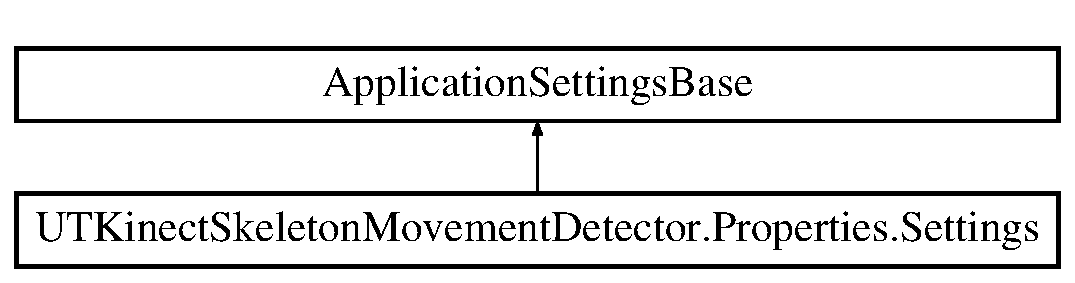
\includegraphics[height=2.000000cm]{classUTKinectSkeletonMovementDetector_1_1Properties_1_1Settings}
\end{center}
\end{figure}
\subsection*{Properties}
\begin{DoxyCompactItemize}
\item 
static \hyperlink{classUTKinectSkeletonMovementDetector_1_1Properties_1_1Settings}{Settings} \hyperlink{classUTKinectSkeletonMovementDetector_1_1Properties_1_1Settings_a0aadb4f47abf4b0b09d34f2f561be8dd}{Default}\hspace{0.3cm}{\ttfamily  \mbox{[}get\mbox{]}}
\end{DoxyCompactItemize}
\subsection*{Static Private Attributes}
\begin{DoxyCompactItemize}
\item 
static \hyperlink{classUTKinectSkeletonMovementDetector_1_1Properties_1_1Settings}{Settings} \hyperlink{classUTKinectSkeletonMovementDetector_1_1Properties_1_1Settings_ae19796fbb92846fa41f12dd457beaa2b}{default\-Instance} = ((\hyperlink{classUTKinectSkeletonMovementDetector_1_1Properties_1_1Settings}{Settings})(global\-::\-System.\-Configuration.\-Application\-Settings\-Base.\-Synchronized(new \hyperlink{classUTKinectSkeletonMovementDetector_1_1Properties_1_1Settings}{Settings}())))
\end{DoxyCompactItemize}


\subsection{Member Data Documentation}
\hypertarget{classUTKinectSkeletonMovementDetector_1_1Properties_1_1Settings_ae19796fbb92846fa41f12dd457beaa2b}{\index{U\-T\-Kinect\-Skeleton\-Movement\-Detector\-::\-Properties\-::\-Settings@{U\-T\-Kinect\-Skeleton\-Movement\-Detector\-::\-Properties\-::\-Settings}!default\-Instance@{default\-Instance}}
\index{default\-Instance@{default\-Instance}!UTKinectSkeletonMovementDetector::Properties::Settings@{U\-T\-Kinect\-Skeleton\-Movement\-Detector\-::\-Properties\-::\-Settings}}
\subsubsection[{default\-Instance}]{\setlength{\rightskip}{0pt plus 5cm}{\bf Settings} U\-T\-Kinect\-Skeleton\-Movement\-Detector.\-Properties.\-Settings.\-default\-Instance = (({\bf Settings})(global\-::\-System.\-Configuration.\-Application\-Settings\-Base.\-Synchronized(new {\bf Settings}())))\hspace{0.3cm}{\ttfamily [static]}, {\ttfamily [private]}}}\label{classUTKinectSkeletonMovementDetector_1_1Properties_1_1Settings_ae19796fbb92846fa41f12dd457beaa2b}


\subsection{Property Documentation}
\hypertarget{classUTKinectSkeletonMovementDetector_1_1Properties_1_1Settings_a0aadb4f47abf4b0b09d34f2f561be8dd}{\index{U\-T\-Kinect\-Skeleton\-Movement\-Detector\-::\-Properties\-::\-Settings@{U\-T\-Kinect\-Skeleton\-Movement\-Detector\-::\-Properties\-::\-Settings}!Default@{Default}}
\index{Default@{Default}!UTKinectSkeletonMovementDetector::Properties::Settings@{U\-T\-Kinect\-Skeleton\-Movement\-Detector\-::\-Properties\-::\-Settings}}
\subsubsection[{Default}]{\setlength{\rightskip}{0pt plus 5cm}{\bf Settings} U\-T\-Kinect\-Skeleton\-Movement\-Detector.\-Properties.\-Settings.\-Default\hspace{0.3cm}{\ttfamily [static]}, {\ttfamily [get]}}}\label{classUTKinectSkeletonMovementDetector_1_1Properties_1_1Settings_a0aadb4f47abf4b0b09d34f2f561be8dd}


The documentation for this class was generated from the following file\-:\begin{DoxyCompactItemize}
\item 
Properties/\hyperlink{Settings_8Designer_8cs}{Settings.\-Designer.\-cs}\end{DoxyCompactItemize}

\hypertarget{classUTKinectSkeletonMovementDetector_1_1SkeletonMovieCreatorWorker}{\section{U\-T\-Kinect\-Skeleton\-Movement\-Detector.\-Skeleton\-Movie\-Creator\-Worker Class Reference}
\label{classUTKinectSkeletonMovementDetector_1_1SkeletonMovieCreatorWorker}\index{U\-T\-Kinect\-Skeleton\-Movement\-Detector.\-Skeleton\-Movie\-Creator\-Worker@{U\-T\-Kinect\-Skeleton\-Movement\-Detector.\-Skeleton\-Movie\-Creator\-Worker}}
}


skeleton movie creation worker class  


\subsection*{Public Member Functions}
\begin{DoxyCompactItemize}
\item 
delegate void \hyperlink{classUTKinectSkeletonMovementDetector_1_1SkeletonMovieCreatorWorker_a688da7c69b3fcbbd1cdb3b9a4cfcb1d7}{On\-Worker\-Method\-Complete\-Delegate} (string message)
\item 
\hyperlink{classUTKinectSkeletonMovementDetector_1_1SkeletonMovieCreatorWorker_aec611bcc2c202380be2b9f47fe846646}{Skeleton\-Movie\-Creator\-Worker} (List$<$ \hyperlink{classUTKinectSkeletonMovementDetector_1_1MySkeletonFrame}{My\-Skeleton\-Frame} $>$ sframes, string \hyperlink{classUTKinectSkeletonMovementDetector_1_1SkeletonMovieCreatorWorker_a75e2c6a66d2a6501da399c2b244140e8}{path})
\item 
void \hyperlink{classUTKinectSkeletonMovementDetector_1_1SkeletonMovieCreatorWorker_a15f5b8ffdfcda85af30cc0a59fc01017}{Worker\-Method} ()
\begin{DoxyCompactList}\small\item\em main worker method \end{DoxyCompactList}\end{DoxyCompactItemize}
\subsection*{Events}
\begin{DoxyCompactItemize}
\item 
\hyperlink{classUTKinectSkeletonMovementDetector_1_1SkeletonMovieCreatorWorker_a688da7c69b3fcbbd1cdb3b9a4cfcb1d7}{On\-Worker\-Method\-Complete\-Delegate} \hyperlink{classUTKinectSkeletonMovementDetector_1_1SkeletonMovieCreatorWorker_a216a708362bfed5567535e47a6124dfb}{On\-Worker\-Complete}
\end{DoxyCompactItemize}
\subsection*{Private Attributes}
\begin{DoxyCompactItemize}
\item 
List$<$ \hyperlink{classUTKinectSkeletonMovementDetector_1_1MySkeletonFrame}{My\-Skeleton\-Frame} $>$ \hyperlink{classUTKinectSkeletonMovementDetector_1_1SkeletonMovieCreatorWorker_a6208ad919e52a106e5f1b9d0988f5c1e}{skeletonframes}
\item 
string \hyperlink{classUTKinectSkeletonMovementDetector_1_1SkeletonMovieCreatorWorker_a75e2c6a66d2a6501da399c2b244140e8}{path}
\end{DoxyCompactItemize}


\subsection{Detailed Description}
skeleton movie creation worker class 



\subsection{Constructor \& Destructor Documentation}
\hypertarget{classUTKinectSkeletonMovementDetector_1_1SkeletonMovieCreatorWorker_aec611bcc2c202380be2b9f47fe846646}{\index{U\-T\-Kinect\-Skeleton\-Movement\-Detector\-::\-Skeleton\-Movie\-Creator\-Worker@{U\-T\-Kinect\-Skeleton\-Movement\-Detector\-::\-Skeleton\-Movie\-Creator\-Worker}!Skeleton\-Movie\-Creator\-Worker@{Skeleton\-Movie\-Creator\-Worker}}
\index{Skeleton\-Movie\-Creator\-Worker@{Skeleton\-Movie\-Creator\-Worker}!UTKinectSkeletonMovementDetector::SkeletonMovieCreatorWorker@{U\-T\-Kinect\-Skeleton\-Movement\-Detector\-::\-Skeleton\-Movie\-Creator\-Worker}}
\subsubsection[{Skeleton\-Movie\-Creator\-Worker}]{\setlength{\rightskip}{0pt plus 5cm}U\-T\-Kinect\-Skeleton\-Movement\-Detector.\-Skeleton\-Movie\-Creator\-Worker.\-Skeleton\-Movie\-Creator\-Worker (
\begin{DoxyParamCaption}
\item[{List$<$ {\bf My\-Skeleton\-Frame} $>$}]{sframes, }
\item[{string}]{path}
\end{DoxyParamCaption}
)}}\label{classUTKinectSkeletonMovementDetector_1_1SkeletonMovieCreatorWorker_aec611bcc2c202380be2b9f47fe846646}


\subsection{Member Function Documentation}
\hypertarget{classUTKinectSkeletonMovementDetector_1_1SkeletonMovieCreatorWorker_a688da7c69b3fcbbd1cdb3b9a4cfcb1d7}{\index{U\-T\-Kinect\-Skeleton\-Movement\-Detector\-::\-Skeleton\-Movie\-Creator\-Worker@{U\-T\-Kinect\-Skeleton\-Movement\-Detector\-::\-Skeleton\-Movie\-Creator\-Worker}!On\-Worker\-Method\-Complete\-Delegate@{On\-Worker\-Method\-Complete\-Delegate}}
\index{On\-Worker\-Method\-Complete\-Delegate@{On\-Worker\-Method\-Complete\-Delegate}!UTKinectSkeletonMovementDetector::SkeletonMovieCreatorWorker@{U\-T\-Kinect\-Skeleton\-Movement\-Detector\-::\-Skeleton\-Movie\-Creator\-Worker}}
\subsubsection[{On\-Worker\-Method\-Complete\-Delegate}]{\setlength{\rightskip}{0pt plus 5cm}delegate void U\-T\-Kinect\-Skeleton\-Movement\-Detector.\-Skeleton\-Movie\-Creator\-Worker.\-On\-Worker\-Method\-Complete\-Delegate (
\begin{DoxyParamCaption}
\item[{string}]{message}
\end{DoxyParamCaption}
)}}\label{classUTKinectSkeletonMovementDetector_1_1SkeletonMovieCreatorWorker_a688da7c69b3fcbbd1cdb3b9a4cfcb1d7}
\hypertarget{classUTKinectSkeletonMovementDetector_1_1SkeletonMovieCreatorWorker_a15f5b8ffdfcda85af30cc0a59fc01017}{\index{U\-T\-Kinect\-Skeleton\-Movement\-Detector\-::\-Skeleton\-Movie\-Creator\-Worker@{U\-T\-Kinect\-Skeleton\-Movement\-Detector\-::\-Skeleton\-Movie\-Creator\-Worker}!Worker\-Method@{Worker\-Method}}
\index{Worker\-Method@{Worker\-Method}!UTKinectSkeletonMovementDetector::SkeletonMovieCreatorWorker@{U\-T\-Kinect\-Skeleton\-Movement\-Detector\-::\-Skeleton\-Movie\-Creator\-Worker}}
\subsubsection[{Worker\-Method}]{\setlength{\rightskip}{0pt plus 5cm}void U\-T\-Kinect\-Skeleton\-Movement\-Detector.\-Skeleton\-Movie\-Creator\-Worker.\-Worker\-Method (
\begin{DoxyParamCaption}
{}
\end{DoxyParamCaption}
)}}\label{classUTKinectSkeletonMovementDetector_1_1SkeletonMovieCreatorWorker_a15f5b8ffdfcda85af30cc0a59fc01017}


main worker method 



\subsection{Member Data Documentation}
\hypertarget{classUTKinectSkeletonMovementDetector_1_1SkeletonMovieCreatorWorker_a75e2c6a66d2a6501da399c2b244140e8}{\index{U\-T\-Kinect\-Skeleton\-Movement\-Detector\-::\-Skeleton\-Movie\-Creator\-Worker@{U\-T\-Kinect\-Skeleton\-Movement\-Detector\-::\-Skeleton\-Movie\-Creator\-Worker}!path@{path}}
\index{path@{path}!UTKinectSkeletonMovementDetector::SkeletonMovieCreatorWorker@{U\-T\-Kinect\-Skeleton\-Movement\-Detector\-::\-Skeleton\-Movie\-Creator\-Worker}}
\subsubsection[{path}]{\setlength{\rightskip}{0pt plus 5cm}string U\-T\-Kinect\-Skeleton\-Movement\-Detector.\-Skeleton\-Movie\-Creator\-Worker.\-path\hspace{0.3cm}{\ttfamily [private]}}}\label{classUTKinectSkeletonMovementDetector_1_1SkeletonMovieCreatorWorker_a75e2c6a66d2a6501da399c2b244140e8}
\hypertarget{classUTKinectSkeletonMovementDetector_1_1SkeletonMovieCreatorWorker_a6208ad919e52a106e5f1b9d0988f5c1e}{\index{U\-T\-Kinect\-Skeleton\-Movement\-Detector\-::\-Skeleton\-Movie\-Creator\-Worker@{U\-T\-Kinect\-Skeleton\-Movement\-Detector\-::\-Skeleton\-Movie\-Creator\-Worker}!skeletonframes@{skeletonframes}}
\index{skeletonframes@{skeletonframes}!UTKinectSkeletonMovementDetector::SkeletonMovieCreatorWorker@{U\-T\-Kinect\-Skeleton\-Movement\-Detector\-::\-Skeleton\-Movie\-Creator\-Worker}}
\subsubsection[{skeletonframes}]{\setlength{\rightskip}{0pt plus 5cm}List$<${\bf My\-Skeleton\-Frame}$>$ U\-T\-Kinect\-Skeleton\-Movement\-Detector.\-Skeleton\-Movie\-Creator\-Worker.\-skeletonframes\hspace{0.3cm}{\ttfamily [private]}}}\label{classUTKinectSkeletonMovementDetector_1_1SkeletonMovieCreatorWorker_a6208ad919e52a106e5f1b9d0988f5c1e}


\subsection{Event Documentation}
\hypertarget{classUTKinectSkeletonMovementDetector_1_1SkeletonMovieCreatorWorker_a216a708362bfed5567535e47a6124dfb}{\index{U\-T\-Kinect\-Skeleton\-Movement\-Detector\-::\-Skeleton\-Movie\-Creator\-Worker@{U\-T\-Kinect\-Skeleton\-Movement\-Detector\-::\-Skeleton\-Movie\-Creator\-Worker}!On\-Worker\-Complete@{On\-Worker\-Complete}}
\index{On\-Worker\-Complete@{On\-Worker\-Complete}!UTKinectSkeletonMovementDetector::SkeletonMovieCreatorWorker@{U\-T\-Kinect\-Skeleton\-Movement\-Detector\-::\-Skeleton\-Movie\-Creator\-Worker}}
\subsubsection[{On\-Worker\-Complete}]{\setlength{\rightskip}{0pt plus 5cm}{\bf On\-Worker\-Method\-Complete\-Delegate} U\-T\-Kinect\-Skeleton\-Movement\-Detector.\-Skeleton\-Movie\-Creator\-Worker.\-On\-Worker\-Complete}}\label{classUTKinectSkeletonMovementDetector_1_1SkeletonMovieCreatorWorker_a216a708362bfed5567535e47a6124dfb}


The documentation for this class was generated from the following file\-:\begin{DoxyCompactItemize}
\item 
\hyperlink{SkeletonMovieCreatorWorker_8cs}{Skeleton\-Movie\-Creator\-Worker.\-cs}\end{DoxyCompactItemize}

\hypertarget{classUTKinectSkeletonMovementDetector_1_1SkeletonPainter}{\section{U\-T\-Kinect\-Skeleton\-Movement\-Detector.\-Skeleton\-Painter Class Reference}
\label{classUTKinectSkeletonMovementDetector_1_1SkeletonPainter}\index{U\-T\-Kinect\-Skeleton\-Movement\-Detector.\-Skeleton\-Painter@{U\-T\-Kinect\-Skeleton\-Movement\-Detector.\-Skeleton\-Painter}}
}
\subsection*{Static Public Member Functions}
\begin{DoxyCompactItemize}
\item 
static System.\-Drawing.\-Image \hyperlink{classUTKinectSkeletonMovementDetector_1_1SkeletonPainter_a7fdb142bafc43845084ae2208ad98ed4}{paintonblank} (Skeleton\mbox{[}$\,$\mbox{]} skeletons)
\begin{DoxyCompactList}\small\item\em draw on a blank black frame \end{DoxyCompactList}\item 
static System.\-Drawing.\-Image \hyperlink{classUTKinectSkeletonMovementDetector_1_1SkeletonPainter_a75e75c7dc95899e548e0b294cd164c3b}{paint\-Skeleton\-And\-Hide\-Head} (Image img, Skeleton\mbox{[}$\,$\mbox{]} skeletons)
\begin{DoxyCompactList}\small\item\em draw on an img \end{DoxyCompactList}\item 
static System.\-Drawing.\-Image \hyperlink{classUTKinectSkeletonMovementDetector_1_1SkeletonPainter_ad4f37b20c059cd693d3e557aeee44377}{hide\-Head} (Image img, Skeleton\mbox{[}$\,$\mbox{]} skeletons)
\begin{DoxyCompactList}\small\item\em draw on a background and also hide head \end{DoxyCompactList}\end{DoxyCompactItemize}
\subsection*{Static Private Member Functions}
\begin{DoxyCompactItemize}
\item 
static Point \hyperlink{classUTKinectSkeletonMovementDetector_1_1SkeletonPainter_ab0533b91ac7ce48bdea5a46aa20b16a8}{get\-Head\-Cover\-Size} (double headz)
\begin{DoxyCompactList}\small\item\em returns the the size of head cover square \end{DoxyCompactList}\item 
static System.\-Drawing.\-Image \hyperlink{classUTKinectSkeletonMovementDetector_1_1SkeletonPainter_a85f7fa7db7126626c9ab4b4ccd01ae1a}{paint} (Image bg, Skeleton\mbox{[}$\,$\mbox{]} skeletons, Point initsize, double proportion, Boolean paintskeleton, Boolean hidehead)
\begin{DoxyCompactList}\small\item\em simply converts a 3d point to display on 640 $\ast$ 480 \-: 2d frame \end{DoxyCompactList}\end{DoxyCompactItemize}


\subsection{Member Function Documentation}
\hypertarget{classUTKinectSkeletonMovementDetector_1_1SkeletonPainter_ab0533b91ac7ce48bdea5a46aa20b16a8}{\index{U\-T\-Kinect\-Skeleton\-Movement\-Detector\-::\-Skeleton\-Painter@{U\-T\-Kinect\-Skeleton\-Movement\-Detector\-::\-Skeleton\-Painter}!get\-Head\-Cover\-Size@{get\-Head\-Cover\-Size}}
\index{get\-Head\-Cover\-Size@{get\-Head\-Cover\-Size}!UTKinectSkeletonMovementDetector::SkeletonPainter@{U\-T\-Kinect\-Skeleton\-Movement\-Detector\-::\-Skeleton\-Painter}}
\subsubsection[{get\-Head\-Cover\-Size}]{\setlength{\rightskip}{0pt plus 5cm}static Point U\-T\-Kinect\-Skeleton\-Movement\-Detector.\-Skeleton\-Painter.\-get\-Head\-Cover\-Size (
\begin{DoxyParamCaption}
\item[{double}]{headz}
\end{DoxyParamCaption}
)\hspace{0.3cm}{\ttfamily [static]}, {\ttfamily [private]}}}\label{classUTKinectSkeletonMovementDetector_1_1SkeletonPainter_ab0533b91ac7ce48bdea5a46aa20b16a8}


returns the the size of head cover square 


\begin{DoxyParams}{Parameters}
{\em bg} & frame to draw skeleton on\\
\hline
\end{DoxyParams}
\hypertarget{classUTKinectSkeletonMovementDetector_1_1SkeletonPainter_ad4f37b20c059cd693d3e557aeee44377}{\index{U\-T\-Kinect\-Skeleton\-Movement\-Detector\-::\-Skeleton\-Painter@{U\-T\-Kinect\-Skeleton\-Movement\-Detector\-::\-Skeleton\-Painter}!hide\-Head@{hide\-Head}}
\index{hide\-Head@{hide\-Head}!UTKinectSkeletonMovementDetector::SkeletonPainter@{U\-T\-Kinect\-Skeleton\-Movement\-Detector\-::\-Skeleton\-Painter}}
\subsubsection[{hide\-Head}]{\setlength{\rightskip}{0pt plus 5cm}static System.\-Drawing.\-Image U\-T\-Kinect\-Skeleton\-Movement\-Detector.\-Skeleton\-Painter.\-hide\-Head (
\begin{DoxyParamCaption}
\item[{Image}]{img, }
\item[{Skeleton\mbox{[}$\,$\mbox{]}}]{skeletons}
\end{DoxyParamCaption}
)\hspace{0.3cm}{\ttfamily [static]}}}\label{classUTKinectSkeletonMovementDetector_1_1SkeletonPainter_ad4f37b20c059cd693d3e557aeee44377}


draw on a background and also hide head 


\begin{DoxyParams}{Parameters}
{\em img} & background to draw skeleton on\\
\hline
{\em skeletons} & skeletons to be drawn on the background\\
\hline
\end{DoxyParams}
\hypertarget{classUTKinectSkeletonMovementDetector_1_1SkeletonPainter_a85f7fa7db7126626c9ab4b4ccd01ae1a}{\index{U\-T\-Kinect\-Skeleton\-Movement\-Detector\-::\-Skeleton\-Painter@{U\-T\-Kinect\-Skeleton\-Movement\-Detector\-::\-Skeleton\-Painter}!paint@{paint}}
\index{paint@{paint}!UTKinectSkeletonMovementDetector::SkeletonPainter@{U\-T\-Kinect\-Skeleton\-Movement\-Detector\-::\-Skeleton\-Painter}}
\subsubsection[{paint}]{\setlength{\rightskip}{0pt plus 5cm}static System.\-Drawing.\-Image U\-T\-Kinect\-Skeleton\-Movement\-Detector.\-Skeleton\-Painter.\-paint (
\begin{DoxyParamCaption}
\item[{Image}]{bg, }
\item[{Skeleton\mbox{[}$\,$\mbox{]}}]{skeletons, }
\item[{Point}]{initsize, }
\item[{double}]{proportion, }
\item[{Boolean}]{paintskeleton, }
\item[{Boolean}]{hidehead}
\end{DoxyParamCaption}
)\hspace{0.3cm}{\ttfamily [static]}, {\ttfamily [private]}}}\label{classUTKinectSkeletonMovementDetector_1_1SkeletonPainter_a85f7fa7db7126626c9ab4b4ccd01ae1a}


simply converts a 3d point to display on 640 $\ast$ 480 \-: 2d frame 


\begin{DoxyParams}{Parameters}
{\em bg} & frame to draw skeleton on\\
\hline
{\em skeletons} & all skeletons of a single frmae\\
\hline
{\em initsize} & skeleton frame initial size\\
\hline
{\em proportion} & ratio of skeleton fram scale\\
\hline
{\em paintskeleton} & determines whether or not all skeleton bones should be painted\\
\hline
{\em hidedead} & whether or not the head should be hided with a black square or not\\
\hline
\end{DoxyParams}
\hypertarget{classUTKinectSkeletonMovementDetector_1_1SkeletonPainter_a7fdb142bafc43845084ae2208ad98ed4}{\index{U\-T\-Kinect\-Skeleton\-Movement\-Detector\-::\-Skeleton\-Painter@{U\-T\-Kinect\-Skeleton\-Movement\-Detector\-::\-Skeleton\-Painter}!paintonblank@{paintonblank}}
\index{paintonblank@{paintonblank}!UTKinectSkeletonMovementDetector::SkeletonPainter@{U\-T\-Kinect\-Skeleton\-Movement\-Detector\-::\-Skeleton\-Painter}}
\subsubsection[{paintonblank}]{\setlength{\rightskip}{0pt plus 5cm}static System.\-Drawing.\-Image U\-T\-Kinect\-Skeleton\-Movement\-Detector.\-Skeleton\-Painter.\-paintonblank (
\begin{DoxyParamCaption}
\item[{Skeleton\mbox{[}$\,$\mbox{]}}]{skeletons}
\end{DoxyParamCaption}
)\hspace{0.3cm}{\ttfamily [static]}}}\label{classUTKinectSkeletonMovementDetector_1_1SkeletonPainter_a7fdb142bafc43845084ae2208ad98ed4}


draw on a blank black frame 


\begin{DoxyParams}{Parameters}
{\em skeletons} & skeletons to draw\\
\hline
\end{DoxyParams}
\hypertarget{classUTKinectSkeletonMovementDetector_1_1SkeletonPainter_a75e75c7dc95899e548e0b294cd164c3b}{\index{U\-T\-Kinect\-Skeleton\-Movement\-Detector\-::\-Skeleton\-Painter@{U\-T\-Kinect\-Skeleton\-Movement\-Detector\-::\-Skeleton\-Painter}!paint\-Skeleton\-And\-Hide\-Head@{paint\-Skeleton\-And\-Hide\-Head}}
\index{paint\-Skeleton\-And\-Hide\-Head@{paint\-Skeleton\-And\-Hide\-Head}!UTKinectSkeletonMovementDetector::SkeletonPainter@{U\-T\-Kinect\-Skeleton\-Movement\-Detector\-::\-Skeleton\-Painter}}
\subsubsection[{paint\-Skeleton\-And\-Hide\-Head}]{\setlength{\rightskip}{0pt plus 5cm}static System.\-Drawing.\-Image U\-T\-Kinect\-Skeleton\-Movement\-Detector.\-Skeleton\-Painter.\-paint\-Skeleton\-And\-Hide\-Head (
\begin{DoxyParamCaption}
\item[{Image}]{img, }
\item[{Skeleton\mbox{[}$\,$\mbox{]}}]{skeletons}
\end{DoxyParamCaption}
)\hspace{0.3cm}{\ttfamily [static]}}}\label{classUTKinectSkeletonMovementDetector_1_1SkeletonPainter_a75e75c7dc95899e548e0b294cd164c3b}


draw on an img 


\begin{DoxyParams}{Parameters}
{\em img} & background of the drawing\\
\hline
{\em skeletons} & skeletons to be drawn on the background\\
\hline
\end{DoxyParams}


The documentation for this class was generated from the following file\-:\begin{DoxyCompactItemize}
\item 
\hyperlink{SkeletonPainter_8cs}{Skeleton\-Painter.\-cs}\end{DoxyCompactItemize}

\hypertarget{classUTKinectSkeletonMovementDetector_1_1SkeletonPointConverter}{\section{U\-T\-Kinect\-Skeleton\-Movement\-Detector.\-Skeleton\-Point\-Converter Class Reference}
\label{classUTKinectSkeletonMovementDetector_1_1SkeletonPointConverter}\index{U\-T\-Kinect\-Skeleton\-Movement\-Detector.\-Skeleton\-Point\-Converter@{U\-T\-Kinect\-Skeleton\-Movement\-Detector.\-Skeleton\-Point\-Converter}}
}


conversion logic for converting 3d skeleton points to 2d  


\subsection*{Static Public Member Functions}
\begin{DoxyCompactItemize}
\item 
static Point \hyperlink{classUTKinectSkeletonMovementDetector_1_1SkeletonPointConverter_a157fd1dacf2febbac43e5f7d73e68714}{convert} (Skeleton\-Point skelpoint)
\begin{DoxyCompactList}\small\item\em simply converts a 3d point to display on 640 $\ast$ 480 \-: 2d frame \end{DoxyCompactList}\item 
static Point \hyperlink{classUTKinectSkeletonMovementDetector_1_1SkeletonPointConverter_a4c80e4c9498cf339d1c70b067852a51c}{convert\-And\-Scale} (Skeleton\-Point skelpoint, Point init\-\_\-size, double ratio)
\begin{DoxyCompactList}\small\item\em without this skeleton and color frames does not coinside completely \end{DoxyCompactList}\end{DoxyCompactItemize}


\subsection{Detailed Description}
conversion logic for converting 3d skeleton points to 2d 



\subsection{Member Function Documentation}
\hypertarget{classUTKinectSkeletonMovementDetector_1_1SkeletonPointConverter_a157fd1dacf2febbac43e5f7d73e68714}{\index{U\-T\-Kinect\-Skeleton\-Movement\-Detector\-::\-Skeleton\-Point\-Converter@{U\-T\-Kinect\-Skeleton\-Movement\-Detector\-::\-Skeleton\-Point\-Converter}!convert@{convert}}
\index{convert@{convert}!UTKinectSkeletonMovementDetector::SkeletonPointConverter@{U\-T\-Kinect\-Skeleton\-Movement\-Detector\-::\-Skeleton\-Point\-Converter}}
\subsubsection[{convert}]{\setlength{\rightskip}{0pt plus 5cm}static Point U\-T\-Kinect\-Skeleton\-Movement\-Detector.\-Skeleton\-Point\-Converter.\-convert (
\begin{DoxyParamCaption}
\item[{Skeleton\-Point}]{skelpoint}
\end{DoxyParamCaption}
)\hspace{0.3cm}{\ttfamily [static]}}}\label{classUTKinectSkeletonMovementDetector_1_1SkeletonPointConverter_a157fd1dacf2febbac43e5f7d73e68714}


simply converts a 3d point to display on 640 $\ast$ 480 \-: 2d frame 

\hypertarget{classUTKinectSkeletonMovementDetector_1_1SkeletonPointConverter_a4c80e4c9498cf339d1c70b067852a51c}{\index{U\-T\-Kinect\-Skeleton\-Movement\-Detector\-::\-Skeleton\-Point\-Converter@{U\-T\-Kinect\-Skeleton\-Movement\-Detector\-::\-Skeleton\-Point\-Converter}!convert\-And\-Scale@{convert\-And\-Scale}}
\index{convert\-And\-Scale@{convert\-And\-Scale}!UTKinectSkeletonMovementDetector::SkeletonPointConverter@{U\-T\-Kinect\-Skeleton\-Movement\-Detector\-::\-Skeleton\-Point\-Converter}}
\subsubsection[{convert\-And\-Scale}]{\setlength{\rightskip}{0pt plus 5cm}static Point U\-T\-Kinect\-Skeleton\-Movement\-Detector.\-Skeleton\-Point\-Converter.\-convert\-And\-Scale (
\begin{DoxyParamCaption}
\item[{Skeleton\-Point}]{skelpoint, }
\item[{Point}]{init\-\_\-size, }
\item[{double}]{ratio}
\end{DoxyParamCaption}
)\hspace{0.3cm}{\ttfamily [static]}}}\label{classUTKinectSkeletonMovementDetector_1_1SkeletonPointConverter_a4c80e4c9498cf339d1c70b067852a51c}


without this skeleton and color frames does not coinside completely 



The documentation for this class was generated from the following file\-:\begin{DoxyCompactItemize}
\item 
\hyperlink{SkeletonPointConverter_8cs}{Skeleton\-Point\-Converter.\-cs}\end{DoxyCompactItemize}

\hypertarget{classWpfApplication4_1_1Window1}{\section{Wpf\-Application4.\-Window1 Class Reference}
\label{classWpfApplication4_1_1Window1}\index{Wpf\-Application4.\-Window1@{Wpf\-Application4.\-Window1}}
}


\hyperlink{classWpfApplication4_1_1Window1}{Window1}  


Inheritance diagram for Wpf\-Application4.\-Window1\-:\begin{figure}[H]
\begin{center}
\leavevmode
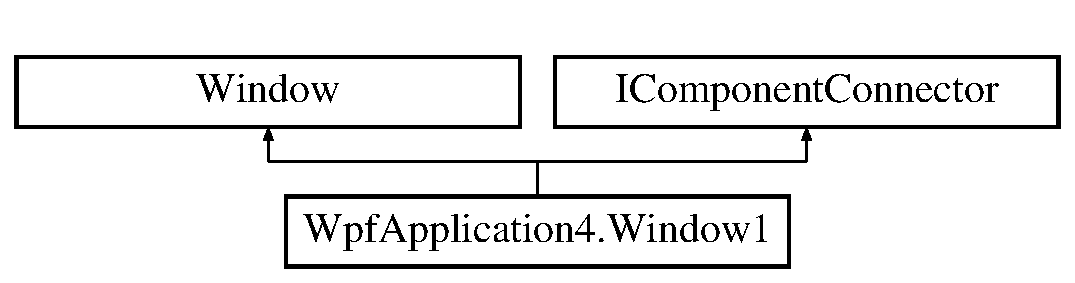
\includegraphics[height=2.000000cm]{classWpfApplication4_1_1Window1}
\end{center}
\end{figure}
\subsection*{Public Member Functions}
\begin{DoxyCompactItemize}
\item 
void \hyperlink{classWpfApplication4_1_1Window1_a6995404d0d7e297f145b6d768e4b2a43}{Initialize\-Component} ()
\begin{DoxyCompactList}\small\item\em Initialize\-Component \end{DoxyCompactList}\end{DoxyCompactItemize}
\subsection*{Private Member Functions}
\begin{DoxyCompactItemize}
\item 
void \\*
System.\-Windows.\-Markup.\-I\-Component\-Connector. \hyperlink{classWpfApplication4_1_1Window1_abced669e1658dafc7f6d4e05eac7f6cc}{Connect} (int connection\-Id, object target)
\end{DoxyCompactItemize}
\subsection*{Private Attributes}
\begin{DoxyCompactItemize}
\item 
bool \hyperlink{classWpfApplication4_1_1Window1_aaba1ddab2801ca465abb0092ccc6c6bf}{\-\_\-content\-Loaded}
\end{DoxyCompactItemize}


\subsection{Detailed Description}
\hyperlink{classWpfApplication4_1_1Window1}{Window1} 



\subsection{Member Function Documentation}
\hypertarget{classWpfApplication4_1_1Window1_abced669e1658dafc7f6d4e05eac7f6cc}{\index{Wpf\-Application4\-::\-Window1@{Wpf\-Application4\-::\-Window1}!Connect@{Connect}}
\index{Connect@{Connect}!WpfApplication4::Window1@{Wpf\-Application4\-::\-Window1}}
\subsubsection[{Connect}]{\setlength{\rightskip}{0pt plus 5cm}void System.\-Windows.\-Markup.\-I\-Component\-Connector. Wpf\-Application4.\-Window1.\-Connect (
\begin{DoxyParamCaption}
\item[{int}]{connection\-Id, }
\item[{object}]{target}
\end{DoxyParamCaption}
)\hspace{0.3cm}{\ttfamily [private]}}}\label{classWpfApplication4_1_1Window1_abced669e1658dafc7f6d4e05eac7f6cc}
\hypertarget{classWpfApplication4_1_1Window1_a6995404d0d7e297f145b6d768e4b2a43}{\index{Wpf\-Application4\-::\-Window1@{Wpf\-Application4\-::\-Window1}!Initialize\-Component@{Initialize\-Component}}
\index{Initialize\-Component@{Initialize\-Component}!WpfApplication4::Window1@{Wpf\-Application4\-::\-Window1}}
\subsubsection[{Initialize\-Component}]{\setlength{\rightskip}{0pt plus 5cm}void Wpf\-Application4.\-Window1.\-Initialize\-Component (
\begin{DoxyParamCaption}
{}
\end{DoxyParamCaption}
)}}\label{classWpfApplication4_1_1Window1_a6995404d0d7e297f145b6d768e4b2a43}


Initialize\-Component 



\subsection{Member Data Documentation}
\hypertarget{classWpfApplication4_1_1Window1_aaba1ddab2801ca465abb0092ccc6c6bf}{\index{Wpf\-Application4\-::\-Window1@{Wpf\-Application4\-::\-Window1}!\-\_\-content\-Loaded@{\-\_\-content\-Loaded}}
\index{\-\_\-content\-Loaded@{\-\_\-content\-Loaded}!WpfApplication4::Window1@{Wpf\-Application4\-::\-Window1}}
\subsubsection[{\-\_\-content\-Loaded}]{\setlength{\rightskip}{0pt plus 5cm}bool Wpf\-Application4.\-Window1.\-\_\-content\-Loaded\hspace{0.3cm}{\ttfamily [private]}}}\label{classWpfApplication4_1_1Window1_aaba1ddab2801ca465abb0092ccc6c6bf}


The documentation for this class was generated from the following file\-:\begin{DoxyCompactItemize}
\item 
obj/x86/\-Release/\hyperlink{Window1_8g_8i_8cs}{Window1.\-g.\-i.\-cs}\end{DoxyCompactItemize}

\chapter{File Documentation}
\hypertarget{App_8xaml_8cs}{\section{App.\-xaml.\-cs File Reference}
\label{App_8xaml_8cs}\index{App.\-xaml.\-cs@{App.\-xaml.\-cs}}
}
\subsection*{Classes}
\begin{DoxyCompactItemize}
\item 
class \hyperlink{classUTKinectSkeletonMovementDetector_1_1App}{U\-T\-Kinect\-Skeleton\-Movement\-Detector.\-App}
\begin{DoxyCompactList}\small\item\em Interaction logic for App.\-xaml \end{DoxyCompactList}\end{DoxyCompactItemize}
\subsection*{Namespaces}
\begin{DoxyCompactItemize}
\item 
package \hyperlink{namespaceUTKinectSkeletonMovementDetector}{U\-T\-Kinect\-Skeleton\-Movement\-Detector}
\end{DoxyCompactItemize}

\hypertarget{ColorMovieCreatorWorker_8cs}{\section{Color\-Movie\-Creator\-Worker.\-cs File Reference}
\label{ColorMovieCreatorWorker_8cs}\index{Color\-Movie\-Creator\-Worker.\-cs@{Color\-Movie\-Creator\-Worker.\-cs}}
}
\subsection*{Classes}
\begin{DoxyCompactItemize}
\item 
class \hyperlink{classUTKinectSkeletonMovementDetector_1_1ColorMovieCreatorWorker}{U\-T\-Kinect\-Skeleton\-Movement\-Detector.\-Color\-Movie\-Creator\-Worker}
\begin{DoxyCompactList}\small\item\em color movie creation worker class \end{DoxyCompactList}\end{DoxyCompactItemize}
\subsection*{Namespaces}
\begin{DoxyCompactItemize}
\item 
package \hyperlink{namespaceUTKinectSkeletonMovementDetector}{U\-T\-Kinect\-Skeleton\-Movement\-Detector}
\end{DoxyCompactItemize}

\hypertarget{LogService_8cs}{\section{Log\-Service.\-cs File Reference}
\label{LogService_8cs}\index{Log\-Service.\-cs@{Log\-Service.\-cs}}
}
\subsection*{Classes}
\begin{DoxyCompactItemize}
\item 
class \hyperlink{classUTKinectSkeletonMovementDetector_1_1LogService}{U\-T\-Kinect\-Skeleton\-Movement\-Detector.\-Log\-Service}
\end{DoxyCompactItemize}
\subsection*{Namespaces}
\begin{DoxyCompactItemize}
\item 
package \hyperlink{namespaceUTKinectSkeletonMovementDetector}{U\-T\-Kinect\-Skeleton\-Movement\-Detector}
\end{DoxyCompactItemize}

\hypertarget{MainWindow_8xaml_8cs}{\section{Main\-Window.\-xaml.\-cs File Reference}
\label{MainWindow_8xaml_8cs}\index{Main\-Window.\-xaml.\-cs@{Main\-Window.\-xaml.\-cs}}
}
\subsection*{Classes}
\begin{DoxyCompactItemize}
\item 
class \hyperlink{classUTKinectSkeletonMovementDetector_1_1MainWindow}{U\-T\-Kinect\-Skeleton\-Movement\-Detector.\-Main\-Window}
\begin{DoxyCompactList}\small\item\em Interaction logic for Main\-Window.\-xaml \end{DoxyCompactList}\end{DoxyCompactItemize}
\subsection*{Namespaces}
\begin{DoxyCompactItemize}
\item 
package \hyperlink{namespaceUTKinectSkeletonMovementDetector}{U\-T\-Kinect\-Skeleton\-Movement\-Detector}
\end{DoxyCompactItemize}

\hypertarget{MovementLogCtreationWorker_8cs}{\section{Movement\-Log\-Ctreation\-Worker.\-cs File Reference}
\label{MovementLogCtreationWorker_8cs}\index{Movement\-Log\-Ctreation\-Worker.\-cs@{Movement\-Log\-Ctreation\-Worker.\-cs}}
}
\subsection*{Classes}
\begin{DoxyCompactItemize}
\item 
class \hyperlink{classUTKinectSkeletonMovementDetector_1_1MovementLogCtreationWorker}{U\-T\-Kinect\-Skeleton\-Movement\-Detector.\-Movement\-Log\-Ctreation\-Worker}
\begin{DoxyCompactList}\small\item\em movement log creation worker class \end{DoxyCompactList}\end{DoxyCompactItemize}
\subsection*{Namespaces}
\begin{DoxyCompactItemize}
\item 
package \hyperlink{namespaceUTKinectSkeletonMovementDetector}{U\-T\-Kinect\-Skeleton\-Movement\-Detector}
\end{DoxyCompactItemize}

\hypertarget{MovieCreator_8cs}{\section{Movie\-Creator.\-cs File Reference}
\label{MovieCreator_8cs}\index{Movie\-Creator.\-cs@{Movie\-Creator.\-cs}}
}
\subsection*{Classes}
\begin{DoxyCompactItemize}
\item 
class \hyperlink{classUTKinectSkeletonMovementDetector_1_1MovieCreator}{U\-T\-Kinect\-Skeleton\-Movement\-Detector.\-Movie\-Creator}
\end{DoxyCompactItemize}
\subsection*{Namespaces}
\begin{DoxyCompactItemize}
\item 
package \hyperlink{namespaceUTKinectSkeletonMovementDetector}{U\-T\-Kinect\-Skeleton\-Movement\-Detector}
\end{DoxyCompactItemize}

\hypertarget{MyColorFrame_8cs}{\section{My\-Color\-Frame.\-cs File Reference}
\label{MyColorFrame_8cs}\index{My\-Color\-Frame.\-cs@{My\-Color\-Frame.\-cs}}
}
\subsection*{Classes}
\begin{DoxyCompactItemize}
\item 
class \hyperlink{classUTKinectSkeletonMovementDetector_1_1MyColorFrame}{U\-T\-Kinect\-Skeleton\-Movement\-Detector.\-My\-Color\-Frame}
\end{DoxyCompactItemize}
\subsection*{Namespaces}
\begin{DoxyCompactItemize}
\item 
package \hyperlink{namespaceUTKinectSkeletonMovementDetector}{U\-T\-Kinect\-Skeleton\-Movement\-Detector}
\end{DoxyCompactItemize}

\hypertarget{MyOverlayFrame_8cs}{\section{My\-Overlay\-Frame.\-cs File Reference}
\label{MyOverlayFrame_8cs}\index{My\-Overlay\-Frame.\-cs@{My\-Overlay\-Frame.\-cs}}
}
\subsection*{Classes}
\begin{DoxyCompactItemize}
\item 
class \hyperlink{classUTKinectSkeletonMovementDetector_1_1MyOverlayFrame}{U\-T\-Kinect\-Skeleton\-Movement\-Detector.\-My\-Overlay\-Frame}
\end{DoxyCompactItemize}
\subsection*{Namespaces}
\begin{DoxyCompactItemize}
\item 
package \hyperlink{namespaceUTKinectSkeletonMovementDetector}{U\-T\-Kinect\-Skeleton\-Movement\-Detector}
\end{DoxyCompactItemize}

\hypertarget{MySkeletonFrame_8cs}{\section{My\-Skeleton\-Frame.\-cs File Reference}
\label{MySkeletonFrame_8cs}\index{My\-Skeleton\-Frame.\-cs@{My\-Skeleton\-Frame.\-cs}}
}
\subsection*{Classes}
\begin{DoxyCompactItemize}
\item 
class \hyperlink{classUTKinectSkeletonMovementDetector_1_1MySkeletonFrame}{U\-T\-Kinect\-Skeleton\-Movement\-Detector.\-My\-Skeleton\-Frame}
\begin{DoxyCompactList}\small\item\em skeleton frame holder \end{DoxyCompactList}\end{DoxyCompactItemize}
\subsection*{Namespaces}
\begin{DoxyCompactItemize}
\item 
package \hyperlink{namespaceUTKinectSkeletonMovementDetector}{U\-T\-Kinect\-Skeleton\-Movement\-Detector}
\end{DoxyCompactItemize}

\hypertarget{Debug_2App_8g_8cs}{\section{obj/x86/\-Debug/\-App.g.\-cs File Reference}
\label{Debug_2App_8g_8cs}\index{obj/x86/\-Debug/\-App.\-g.\-cs@{obj/x86/\-Debug/\-App.\-g.\-cs}}
}
\subsection*{Classes}
\begin{DoxyCompactItemize}
\item 
class \hyperlink{classWpfApplication4_1_1App}{Wpf\-Application4.\-App}
\begin{DoxyCompactList}\small\item\em \hyperlink{classWpfApplication4_1_1App}{App} \end{DoxyCompactList}\end{DoxyCompactItemize}
\subsection*{Namespaces}
\begin{DoxyCompactItemize}
\item 
package \hyperlink{namespaceWpfApplication4}{Wpf\-Application4}
\end{DoxyCompactItemize}

\hypertarget{Release_2App_8g_8cs}{\section{obj/x86/\-Release/\-App.g.\-cs File Reference}
\label{Release_2App_8g_8cs}\index{obj/x86/\-Release/\-App.\-g.\-cs@{obj/x86/\-Release/\-App.\-g.\-cs}}
}
\subsection*{Classes}
\begin{DoxyCompactItemize}
\item 
class \hyperlink{classUTKinectSkeletonMovementDetector_1_1App}{U\-T\-Kinect\-Skeleton\-Movement\-Detector.\-App}
\begin{DoxyCompactList}\small\item\em Interaction logic for App.\-xaml \end{DoxyCompactList}\end{DoxyCompactItemize}
\subsection*{Namespaces}
\begin{DoxyCompactItemize}
\item 
package \hyperlink{namespaceUTKinectSkeletonMovementDetector}{U\-T\-Kinect\-Skeleton\-Movement\-Detector}
\end{DoxyCompactItemize}

\hypertarget{Debug_2App_8g_8i_8cs}{\section{obj/x86/\-Debug/\-App.g.\-i.\-cs File Reference}
\label{Debug_2App_8g_8i_8cs}\index{obj/x86/\-Debug/\-App.\-g.\-i.\-cs@{obj/x86/\-Debug/\-App.\-g.\-i.\-cs}}
}
\subsection*{Classes}
\begin{DoxyCompactItemize}
\item 
class \hyperlink{classWpfApplication4_1_1App}{Wpf\-Application4.\-App}
\begin{DoxyCompactList}\small\item\em \hyperlink{classWpfApplication4_1_1App}{App} \end{DoxyCompactList}\end{DoxyCompactItemize}
\subsection*{Namespaces}
\begin{DoxyCompactItemize}
\item 
package \hyperlink{namespaceWpfApplication4}{Wpf\-Application4}
\end{DoxyCompactItemize}

\hypertarget{Release_2App_8g_8i_8cs}{\section{obj/x86/\-Release/\-App.g.\-i.\-cs File Reference}
\label{Release_2App_8g_8i_8cs}\index{obj/x86/\-Release/\-App.\-g.\-i.\-cs@{obj/x86/\-Release/\-App.\-g.\-i.\-cs}}
}
\subsection*{Classes}
\begin{DoxyCompactItemize}
\item 
class \hyperlink{classUTKinectSkeletonMovementDetector_1_1App}{U\-T\-Kinect\-Skeleton\-Movement\-Detector.\-App}
\begin{DoxyCompactList}\small\item\em Interaction logic for App.\-xaml \end{DoxyCompactList}\end{DoxyCompactItemize}
\subsection*{Namespaces}
\begin{DoxyCompactItemize}
\item 
package \hyperlink{namespaceUTKinectSkeletonMovementDetector}{U\-T\-Kinect\-Skeleton\-Movement\-Detector}
\end{DoxyCompactItemize}

\hypertarget{Debug_2MainWindow_8g_8cs}{\section{obj/x86/\-Debug/\-Main\-Window.g.\-cs File Reference}
\label{Debug_2MainWindow_8g_8cs}\index{obj/x86/\-Debug/\-Main\-Window.\-g.\-cs@{obj/x86/\-Debug/\-Main\-Window.\-g.\-cs}}
}
\subsection*{Classes}
\begin{DoxyCompactItemize}
\item 
class \hyperlink{classWpfApplication4_1_1MainWindow}{Wpf\-Application4.\-Main\-Window}
\begin{DoxyCompactList}\small\item\em \hyperlink{classWpfApplication4_1_1MainWindow}{Main\-Window} \end{DoxyCompactList}\end{DoxyCompactItemize}
\subsection*{Namespaces}
\begin{DoxyCompactItemize}
\item 
package \hyperlink{namespaceWpfApplication4}{Wpf\-Application4}
\end{DoxyCompactItemize}

\hypertarget{Release_2MainWindow_8g_8cs}{\section{obj/x86/\-Release/\-Main\-Window.g.\-cs File Reference}
\label{Release_2MainWindow_8g_8cs}\index{obj/x86/\-Release/\-Main\-Window.\-g.\-cs@{obj/x86/\-Release/\-Main\-Window.\-g.\-cs}}
}
\subsection*{Classes}
\begin{DoxyCompactItemize}
\item 
class \hyperlink{classUTKinectSkeletonMovementDetector_1_1MainWindow}{U\-T\-Kinect\-Skeleton\-Movement\-Detector.\-Main\-Window}
\begin{DoxyCompactList}\small\item\em Interaction logic for Main\-Window.\-xaml \end{DoxyCompactList}\end{DoxyCompactItemize}
\subsection*{Namespaces}
\begin{DoxyCompactItemize}
\item 
package \hyperlink{namespaceUTKinectSkeletonMovementDetector}{U\-T\-Kinect\-Skeleton\-Movement\-Detector}
\end{DoxyCompactItemize}

\hypertarget{Debug_2MainWindow_8g_8i_8cs}{\section{obj/x86/\-Debug/\-Main\-Window.g.\-i.\-cs File Reference}
\label{Debug_2MainWindow_8g_8i_8cs}\index{obj/x86/\-Debug/\-Main\-Window.\-g.\-i.\-cs@{obj/x86/\-Debug/\-Main\-Window.\-g.\-i.\-cs}}
}
\subsection*{Classes}
\begin{DoxyCompactItemize}
\item 
class \hyperlink{classWpfApplication4_1_1MainWindow}{Wpf\-Application4.\-Main\-Window}
\begin{DoxyCompactList}\small\item\em \hyperlink{classWpfApplication4_1_1MainWindow}{Main\-Window} \end{DoxyCompactList}\end{DoxyCompactItemize}
\subsection*{Namespaces}
\begin{DoxyCompactItemize}
\item 
package \hyperlink{namespaceWpfApplication4}{Wpf\-Application4}
\end{DoxyCompactItemize}

\hypertarget{Release_2MainWindow_8g_8i_8cs}{\section{obj/x86/\-Release/\-Main\-Window.g.\-i.\-cs File Reference}
\label{Release_2MainWindow_8g_8i_8cs}\index{obj/x86/\-Release/\-Main\-Window.\-g.\-i.\-cs@{obj/x86/\-Release/\-Main\-Window.\-g.\-i.\-cs}}
}
\subsection*{Classes}
\begin{DoxyCompactItemize}
\item 
class \hyperlink{classUTKinectSkeletonMovementDetector_1_1MainWindow}{U\-T\-Kinect\-Skeleton\-Movement\-Detector.\-Main\-Window}
\begin{DoxyCompactList}\small\item\em Interaction logic for Main\-Window.\-xaml \end{DoxyCompactList}\end{DoxyCompactItemize}
\subsection*{Namespaces}
\begin{DoxyCompactItemize}
\item 
package \hyperlink{namespaceUTKinectSkeletonMovementDetector}{U\-T\-Kinect\-Skeleton\-Movement\-Detector}
\end{DoxyCompactItemize}

\hypertarget{NameDialoge_8g_8i_8cs}{\section{obj/x86/\-Release/\-Name\-Dialoge.g.\-i.\-cs File Reference}
\label{NameDialoge_8g_8i_8cs}\index{obj/x86/\-Release/\-Name\-Dialoge.\-g.\-i.\-cs@{obj/x86/\-Release/\-Name\-Dialoge.\-g.\-i.\-cs}}
}
\subsection*{Classes}
\begin{DoxyCompactItemize}
\item 
class \hyperlink{classWpfApplication4_1_1NameDialoge}{Wpf\-Application4.\-Name\-Dialoge}
\begin{DoxyCompactList}\small\item\em \hyperlink{classWpfApplication4_1_1NameDialoge}{Name\-Dialoge} \end{DoxyCompactList}\end{DoxyCompactItemize}
\subsection*{Namespaces}
\begin{DoxyCompactItemize}
\item 
package \hyperlink{namespaceWpfApplication4}{Wpf\-Application4}
\end{DoxyCompactItemize}

\hypertarget{progressDialog_8g_8cs}{\section{obj/x86/\-Release/progress\-Dialog.g.\-cs File Reference}
\label{progressDialog_8g_8cs}\index{obj/x86/\-Release/progress\-Dialog.\-g.\-cs@{obj/x86/\-Release/progress\-Dialog.\-g.\-cs}}
}
\subsection*{Classes}
\begin{DoxyCompactItemize}
\item 
class \hyperlink{classUTKinectSkeletonMovementDetector_1_1progressDialog}{U\-T\-Kinect\-Skeleton\-Movement\-Detector.\-progress\-Dialog}
\begin{DoxyCompactList}\small\item\em \hyperlink{classUTKinectSkeletonMovementDetector_1_1progressDialog}{progress\-Dialog} \end{DoxyCompactList}\end{DoxyCompactItemize}
\subsection*{Namespaces}
\begin{DoxyCompactItemize}
\item 
package \hyperlink{namespaceUTKinectSkeletonMovementDetector}{U\-T\-Kinect\-Skeleton\-Movement\-Detector}
\end{DoxyCompactItemize}

\hypertarget{progressDialog_8g_8i_8cs}{\section{obj/x86/\-Release/progress\-Dialog.g.\-i.\-cs File Reference}
\label{progressDialog_8g_8i_8cs}\index{obj/x86/\-Release/progress\-Dialog.\-g.\-i.\-cs@{obj/x86/\-Release/progress\-Dialog.\-g.\-i.\-cs}}
}
\subsection*{Classes}
\begin{DoxyCompactItemize}
\item 
class \hyperlink{classUTKinectSkeletonMovementDetector_1_1progressDialog}{U\-T\-Kinect\-Skeleton\-Movement\-Detector.\-progress\-Dialog}
\begin{DoxyCompactList}\small\item\em \hyperlink{classUTKinectSkeletonMovementDetector_1_1progressDialog}{progress\-Dialog} \end{DoxyCompactList}\end{DoxyCompactItemize}
\subsection*{Namespaces}
\begin{DoxyCompactItemize}
\item 
package \hyperlink{namespaceUTKinectSkeletonMovementDetector}{U\-T\-Kinect\-Skeleton\-Movement\-Detector}
\end{DoxyCompactItemize}

\hypertarget{TemporaryGeneratedFile__036C0B5B-1481-4323-8D20-8F5ADCB23D92_8cs}{\section{obj/x86/\-Release/\-Temporary\-Generated\-File\-\_\-036\-C0\-B5\-B-\/1481-\/4323-\/8\-D20-\/8\-F5\-A\-D\-C\-B23\-D92.cs File Reference}
\label{TemporaryGeneratedFile__036C0B5B-1481-4323-8D20-8F5ADCB23D92_8cs}\index{obj/x86/\-Release/\-Temporary\-Generated\-File\-\_\-036\-C0\-B5\-B-\/1481-\/4323-\/8\-D20-\/8\-F5\-A\-D\-C\-B23\-D92.\-cs@{obj/x86/\-Release/\-Temporary\-Generated\-File\-\_\-036\-C0\-B5\-B-\/1481-\/4323-\/8\-D20-\/8\-F5\-A\-D\-C\-B23\-D92.\-cs}}
}

\hypertarget{TemporaryGeneratedFile__5937a670-0e60-4077-877b-f7221da3dda1_8cs}{\section{obj/x86/\-Release/\-Temporary\-Generated\-File\-\_\-5937a670-\/0e60-\/4077-\/877b-\/f7221da3dda1.cs File Reference}
\label{TemporaryGeneratedFile__5937a670-0e60-4077-877b-f7221da3dda1_8cs}\index{obj/x86/\-Release/\-Temporary\-Generated\-File\-\_\-5937a670-\/0e60-\/4077-\/877b-\/f7221da3dda1.\-cs@{obj/x86/\-Release/\-Temporary\-Generated\-File\-\_\-5937a670-\/0e60-\/4077-\/877b-\/f7221da3dda1.\-cs}}
}

\hypertarget{TemporaryGeneratedFile__E7A71F73-0F8D-4B9B-B56E-8E70B10BC5D3_8cs}{\section{obj/x86/\-Release/\-Temporary\-Generated\-File\-\_\-\-E7\-A71\-F73-\/0\-F8\-D-\/4\-B9\-B-\/\-B56\-E-\/8\-E70\-B10\-B\-C5\-D3.cs File Reference}
\label{TemporaryGeneratedFile__E7A71F73-0F8D-4B9B-B56E-8E70B10BC5D3_8cs}\index{obj/x86/\-Release/\-Temporary\-Generated\-File\-\_\-\-E7\-A71\-F73-\/0\-F8\-D-\/4\-B9\-B-\/\-B56\-E-\/8\-E70\-B10\-B\-C5\-D3.\-cs@{obj/x86/\-Release/\-Temporary\-Generated\-File\-\_\-\-E7\-A71\-F73-\/0\-F8\-D-\/4\-B9\-B-\/\-B56\-E-\/8\-E70\-B10\-B\-C5\-D3.\-cs}}
}

\hypertarget{Window1_8g_8i_8cs}{\section{obj/x86/\-Release/\-Window1.g.\-i.\-cs File Reference}
\label{Window1_8g_8i_8cs}\index{obj/x86/\-Release/\-Window1.\-g.\-i.\-cs@{obj/x86/\-Release/\-Window1.\-g.\-i.\-cs}}
}
\subsection*{Classes}
\begin{DoxyCompactItemize}
\item 
class \hyperlink{classWpfApplication4_1_1Window1}{Wpf\-Application4.\-Window1}
\begin{DoxyCompactList}\small\item\em \hyperlink{classWpfApplication4_1_1Window1}{Window1} \end{DoxyCompactList}\end{DoxyCompactItemize}
\subsection*{Namespaces}
\begin{DoxyCompactItemize}
\item 
package \hyperlink{namespaceWpfApplication4}{Wpf\-Application4}
\end{DoxyCompactItemize}

\hypertarget{WpfApplication4__Content_8g_8i_8cs}{\section{obj/x86/\-Release/\-Wpf\-Application4\-\_\-\-Content.g.\-i.\-cs File Reference}
\label{WpfApplication4__Content_8g_8i_8cs}\index{obj/x86/\-Release/\-Wpf\-Application4\-\_\-\-Content.\-g.\-i.\-cs@{obj/x86/\-Release/\-Wpf\-Application4\-\_\-\-Content.\-g.\-i.\-cs}}
}

\hypertarget{OverlayMovieCreatorWorker_8cs}{\section{Overlay\-Movie\-Creator\-Worker.\-cs File Reference}
\label{OverlayMovieCreatorWorker_8cs}\index{Overlay\-Movie\-Creator\-Worker.\-cs@{Overlay\-Movie\-Creator\-Worker.\-cs}}
}
\subsection*{Classes}
\begin{DoxyCompactItemize}
\item 
class \hyperlink{classUTKinectSkeletonMovementDetector_1_1OverlayMovieCreatorWorker}{U\-T\-Kinect\-Skeleton\-Movement\-Detector.\-Overlay\-Movie\-Creator\-Worker}
\begin{DoxyCompactList}\small\item\em overlay movie creation worker class \end{DoxyCompactList}\end{DoxyCompactItemize}
\subsection*{Namespaces}
\begin{DoxyCompactItemize}
\item 
package \hyperlink{namespaceUTKinectSkeletonMovementDetector}{U\-T\-Kinect\-Skeleton\-Movement\-Detector}
\end{DoxyCompactItemize}

\hypertarget{progressDialog_8xaml_8cs}{\section{progress\-Dialog.\-xaml.\-cs File Reference}
\label{progressDialog_8xaml_8cs}\index{progress\-Dialog.\-xaml.\-cs@{progress\-Dialog.\-xaml.\-cs}}
}
\subsection*{Classes}
\begin{DoxyCompactItemize}
\item 
class \hyperlink{classUTKinectSkeletonMovementDetector_1_1progressDialog}{U\-T\-Kinect\-Skeleton\-Movement\-Detector.\-progress\-Dialog}
\begin{DoxyCompactList}\small\item\em \hyperlink{classUTKinectSkeletonMovementDetector_1_1progressDialog}{progress\-Dialog} \end{DoxyCompactList}\end{DoxyCompactItemize}
\subsection*{Namespaces}
\begin{DoxyCompactItemize}
\item 
package \hyperlink{namespaceUTKinectSkeletonMovementDetector}{U\-T\-Kinect\-Skeleton\-Movement\-Detector}
\end{DoxyCompactItemize}

\hypertarget{AssemblyInfo_8cs}{\section{Properties/\-Assembly\-Info.cs File Reference}
\label{AssemblyInfo_8cs}\index{Properties/\-Assembly\-Info.\-cs@{Properties/\-Assembly\-Info.\-cs}}
}

\hypertarget{Resources_8Designer_8cs}{\section{Properties/\-Resources.Designer.\-cs File Reference}
\label{Resources_8Designer_8cs}\index{Properties/\-Resources.\-Designer.\-cs@{Properties/\-Resources.\-Designer.\-cs}}
}
\subsection*{Classes}
\begin{DoxyCompactItemize}
\item 
class \hyperlink{classUTKinectSkeletonMovementDetector_1_1Properties_1_1Resources}{U\-T\-Kinect\-Skeleton\-Movement\-Detector.\-Properties.\-Resources}
\begin{DoxyCompactList}\small\item\em A strongly-\/typed resource class, for looking up localized strings, etc. \end{DoxyCompactList}\end{DoxyCompactItemize}
\subsection*{Namespaces}
\begin{DoxyCompactItemize}
\item 
package \hyperlink{namespaceUTKinectSkeletonMovementDetector_1_1Properties}{U\-T\-Kinect\-Skeleton\-Movement\-Detector.\-Properties}
\end{DoxyCompactItemize}

\hypertarget{Settings_8Designer_8cs}{\section{Properties/\-Settings.Designer.\-cs File Reference}
\label{Settings_8Designer_8cs}\index{Properties/\-Settings.\-Designer.\-cs@{Properties/\-Settings.\-Designer.\-cs}}
}
\subsection*{Classes}
\begin{DoxyCompactItemize}
\item 
class \hyperlink{classUTKinectSkeletonMovementDetector_1_1Properties_1_1Settings}{U\-T\-Kinect\-Skeleton\-Movement\-Detector.\-Properties.\-Settings}
\end{DoxyCompactItemize}
\subsection*{Namespaces}
\begin{DoxyCompactItemize}
\item 
package \hyperlink{namespaceUTKinectSkeletonMovementDetector_1_1Properties}{U\-T\-Kinect\-Skeleton\-Movement\-Detector.\-Properties}
\end{DoxyCompactItemize}

\hypertarget{SkeletonMovieCreatorWorker_8cs}{\section{Skeleton\-Movie\-Creator\-Worker.\-cs File Reference}
\label{SkeletonMovieCreatorWorker_8cs}\index{Skeleton\-Movie\-Creator\-Worker.\-cs@{Skeleton\-Movie\-Creator\-Worker.\-cs}}
}
\subsection*{Classes}
\begin{DoxyCompactItemize}
\item 
class \hyperlink{classUTKinectSkeletonMovementDetector_1_1SkeletonMovieCreatorWorker}{U\-T\-Kinect\-Skeleton\-Movement\-Detector.\-Skeleton\-Movie\-Creator\-Worker}
\begin{DoxyCompactList}\small\item\em skeleton movie creation worker class \end{DoxyCompactList}\end{DoxyCompactItemize}
\subsection*{Namespaces}
\begin{DoxyCompactItemize}
\item 
package \hyperlink{namespaceUTKinectSkeletonMovementDetector}{U\-T\-Kinect\-Skeleton\-Movement\-Detector}
\end{DoxyCompactItemize}

\hypertarget{SkeletonPainter_8cs}{\section{Skeleton\-Painter.\-cs File Reference}
\label{SkeletonPainter_8cs}\index{Skeleton\-Painter.\-cs@{Skeleton\-Painter.\-cs}}
}
\subsection*{Classes}
\begin{DoxyCompactItemize}
\item 
class \hyperlink{classUTKinectSkeletonMovementDetector_1_1SkeletonPainter}{U\-T\-Kinect\-Skeleton\-Movement\-Detector.\-Skeleton\-Painter}
\end{DoxyCompactItemize}
\subsection*{Namespaces}
\begin{DoxyCompactItemize}
\item 
package \hyperlink{namespaceUTKinectSkeletonMovementDetector}{U\-T\-Kinect\-Skeleton\-Movement\-Detector}
\end{DoxyCompactItemize}

\hypertarget{SkeletonPointConverter_8cs}{\section{Skeleton\-Point\-Converter.\-cs File Reference}
\label{SkeletonPointConverter_8cs}\index{Skeleton\-Point\-Converter.\-cs@{Skeleton\-Point\-Converter.\-cs}}
}
\subsection*{Classes}
\begin{DoxyCompactItemize}
\item 
class \hyperlink{classUTKinectSkeletonMovementDetector_1_1SkeletonPointConverter}{U\-T\-Kinect\-Skeleton\-Movement\-Detector.\-Skeleton\-Point\-Converter}
\begin{DoxyCompactList}\small\item\em conversion logic for converting 3d skeleton points to 2d \end{DoxyCompactList}\end{DoxyCompactItemize}
\subsection*{Namespaces}
\begin{DoxyCompactItemize}
\item 
package \hyperlink{namespaceUTKinectSkeletonMovementDetector}{U\-T\-Kinect\-Skeleton\-Movement\-Detector}
\end{DoxyCompactItemize}

%--- End generated contents ---

% Index
\newpage
\phantomsection
\addcontentsline{toc}{chapter}{Index}
\printindex

\end{document}
